\documentclass[11pt]{article}%\RequirePackage{snapshot}    %% to generate the .dep file
\usepackage{times}
\usepackage[comma]{natbib}
\usepackage{url}
\usepackage{bm}
\usepackage{graphicx}
\usepackage{epigraph}
\usepackage{comment}
\usepackage{mdwlist}
\usepackage{amsmath}
\usepackage{amssymb}
\usepackage{latexsym}        %% LaTeX symbols: \Box, etc.th}
\usepackage{color}

\bibliographystyle{styles/abbrvnat-apa-nourl}

%% \bibliographystyle{apalike} % for John

% Only to include a page header on the first page for preprints
%\usepackage{afterpage}
%\usepackage{fancyhdr}

%  Abbreviations for cross-references
\newcommand*{\figref}[1]{Figure~\ref{#1}}
\newcommand*{\tabref}[1]{Table~\ref{#1}}
\newcommand*{\secref}[1]{Section~\ref{#1}}
\renewcommand*{\eqref}[1]{Eqn.~(\ref{#1})}


\newcommand{\keywords}[1]{\par\noindent\textbf{Key words:} #1}
\newcommand*{\todo}[1]{\marginpar{ToDo:\small{#1}}}
\newcommand{\TODO}[1]{\begin{quotation}\noindent\color{blue}\textbf{ToDo}: #1\end{quotation}}


%  Page dimensions
\addtolength{\hoffset}{-2cm}
\addtolength{\textwidth}{4cm}
\addtolength{\voffset}{-2cm}
\addtolength{\textheight}{4cm}

% Math stuff
%   vector and matrix expressions
\renewcommand*{\vec}[1]{\ensuremath{\bm{#1}}}     % \vec{} is already used 
\newcommand*{\mat}[1]{\ensuremath{\bm{#1}}}
%\newcommand{\trans}{\ensuremath{'}}
\newcommand{\trans}{\ensuremath{^\mathsf{T}}}
\newcommand*{\diag}[1]{\ensuremath{\mathrm{diag}\, #1}}
\renewcommand*{\det}[1]{\ensuremath{\mathrm{det} (#1)}}
\newcommand*{\detbracket}[1]{\ensuremath{\mathrm{det} [#1]}}
\newcommand*{\rank}[1]{\ensuremath{\mathrm{rank} (\mat{#1})}}
\newcommand*{\trace}[1]{\ensuremath{\mathrm{tr} (\mat{#1})}}
\newcommand*{\dev}[1]{(#1 - \bar{#1})}
\newcommand*{\inv}[1]{\ensuremath{\mat{#1}^{-1}}}
\newcommand*{\half}[1]{\ensuremath{\mat{#1}^{1/2}}}
\newcommand*{\invhalf}[1]{\ensuremath{\mat{#1}^{-1/2}}}
\newcommand*{\nvec}[2]{\ensuremath{{#1}_{1}, {#1}_{2},\ldots,{#1}_{#2}}}
\newcommand*{\given}{\ensuremath{\, | \,}}
\newcommand*{\Beta}{B}
\newcommand*{\Epsilon}{E}
%    punctuation in display equations
\newcommand*{\period}{\:\: .}   
\newcommand*{\comma}{\:\: ,}

\newcommand*{\Real}[1]{\mathbb{R}^{#1}}     % nicer looking than \Re
\newcommand*{\degree}[1]{\ensuremath{{#1}^{\circ}}}
\newcommand{\sizedmat}[2]{%
  \mathord{\mathop{\mat{#1}}\limits_{(#2)}}%
}
\newcommand{\Var}{\ensuremath{\mathsf{Var}}}
\newcommand{\Cov}{\ensuremath{\mathsf{Cov}}}
\newcommand{\argmin}{\mathop{\mathrm{argmin}}}


% abbreviations
\newcommand{\MLM}{MvLM}

% shorthand for including simple figures
%   \fig{name}{includegraphicsoptions}{caption}
\newcommand{\fig}[3]{%
\begin{figure}[!htb]
  \centering%
  \includegraphics[#2]{fig/#1}%
  \caption{#3}%
  \label{fig:#1}
\end{figure}
}

% set width for \epigraph{}{}
\setlength{\epigraphwidth}{.9\textwidth}

\begin{document}
\begin{titlepage}
\title{Elliptical Insights: Understanding Statistical Methods through Elliptical Geometry}

\author{Michael Friendly%
%\thanks{Michael Friendly is Professor, Psychology Department,
%York University, Toronto, ON, M3J 1P3 Canada, E-mail: friendly@yorku.ca.}
 \\ York University
\and
Georges Monette \\ York University
\and
John Fox \\ McMaster University
}
\date{Draft v. 0.9-1, \today}
\end{titlepage}
\maketitle
%\thispagestyle{fancy}\lhead{In press: \emph{Journal of Computational and Statistical Graphics}, 2001}\rhead{}\afterpage{\lhead{}\rhead{}}

\begin{abstract}
Visual insights into  a wide variety  of statistical methods,  for both didactic
and data analytic purposes, can often be achieved through geometric diagrams  and
geometrically based statistical graphs.  This  paper extols and illustrates  the
virtues  of  the  ellipse  and her  higher-dimensional  cousins  for  both these
purposes in a variety of contexts, including linear models, multivariate
linear models, and mixed-effect models.
We emphasize the strong relations among statistical methods, matrix-algebraic
solutions, and geometry that can often be easily understood in terms of
ellipses.
%Most of the statistical methods we discuss stem,
%at least implicitly, from classic Gaussian assumptions. But, to whatever extent the
%We survey a wide number of statistical problems in which

\keywords{
added-variable plots;
Bayesian estimation;
concentration ellipse;
data ellipse;
discriminant analysis;
Francis Galton;
hypothesis-error plots;
measurement error;
mixed-effect models;
regression paradoxes;
ridge regression;
statistical geometry
}
\end{abstract}

\section{Introduction}

\epigraph{Whatever relates to extent and quantity may be represented by
geometrical figures. Statistical projections which speak to the senses without
fatiguing the mind, possess the advantage of fixing the attention on a great
number of important facts.}{Alexander von Humboldt \citeyearpar[p.~ciii]{Humboldt:1811a}}

In the beginning (of modern  statistical methods), there was the  ellipse. As statistical
methods progressed from bivariate to multivariate, the ellipse escaped the plane to a 3D
ellipsoid, and then onwards to higher dimensions.
This  paper extols and illustrates the
virtues of the ellipse and her higher-dimensional cousins for both didactic and
data analytic purposes.

When
Francis Galton  \citeyearpar{Galton:1886} first  studied the  relationship between  heritable traits of
parents and their offspring, he  had a remarkable visual insight--- contours of
equal bivariate frequencies in the joint distribution seemed to form  concentric
shapes whose outlines  were, to Galton,  tolerably close to  concentric ellipses
differing only in scale.

Galton's goal was to  to predict (or explain)  how a characteristic, $Y$,   (e.g.,
height) of children was  related to that of  their parents, $X$.  To  this end, he
calculated summaries,  $\mathrm{Ave}(Y\given X)$,  and, for  symmetry, $\mathrm{Ave}(X\given Y)$, and plotted
these as lines of means on his  diagram.  Lo and behold, he had a  second visual
insight:  the lines  of means of  ($Y\given X$) and ($X\given Y$)  corresponded approximately to
the locus of  horizontal and vertical  tangents to the  concentric ellipses.  To
complete the picture,  he added lines  showing the major  and minor axes  of the
family of ellipses, with the result shown in Figure 1.

It is  not stretching  the point  too far  to say  that a  large part  of modern
statistical  methods  descend  from  these  visual  insights:%
\footnote{\citet[p. 37]{Pearson:1920} later stated, ``that Galton
should have evolved all this from his observations is to my mind one
of the most noteworthy scientific discoveries arising from pure
analysis of observations.'' }
correlation   and
regression \citep{Pearson:1896}, the  bivariate normal  distribution,
and principal components  \citep{Pearson:1901,Hotelling:1933}  all trace their ancestry to Galton's  geometrical
diagram.%
\footnote{
Well, not entirely. Auguste Bravais [1811--1863] \citeyearpar{Bravais:1846}, an astronomer
and physicist first introduced the mathematical theory of the bivariate normal distribution
as a model for the joint frequency of errors in the geometric position of a point.
Bravais derived the formula for level slices as concentric ellipses and had a rudimentary
notion of correlation but did not appreciate this as a representation of data.
Nonetheless, \cite{Pearson:1920} acknowledged Bravais's contribution, and the correlation
coefficient is often called the Bravais-Pearson coefficient in France
\citep{Denis:2001}. }
%\todo{Ref: Denis}


Basic geometry goes back at least to Euclid, but the properties of the ellipse and  other
conic sections may be traced to Apollonius  of Perga (ca.~262 BC--ca.~190 BC),  a
Greek geometer and astronomer who gave the ellipse, parabola, and hyperbola their
modern names. In a work popularly called the Conics \citep{Boyer:91}, he  described
the  fundamental  properties  of  ellipses  (eccentricity,  axes,  principles of
tange+ncy,  normals as  minimum and  maximum straight  lines to  the curve)  with
remarkable clarity nearly 2000 years before the development of analytic geometry
by Descartes.

% one figure
\begin{figure}[htb]
  \centering
  \includegraphics[width=.65\textwidth]{fig/galton-corr}
  \caption{Galton's 1886 diagram, showing the relationship of height of children
to the average of their parents' height. The diagram is essentially an overlay
of a geometrical interpretation on a bivariate grouped frequency distribution, shown
as numbers.}%
  \label{fig:galton-corr}
\end{figure}

Over time, the ellipse would be called to duty to provide simple explanations of
phenomena  once thought  complex.  Most  notable is  Kepler's insight  that the
Copernican theory of the orbits of planets as concentric circles (which required
notions  of  epicycles  to  account  for  observations)  could  be  brought into
alignment with the detailed observations by  Tycho Brahe and others by a  simple
law: ``The orbit  of every planet  is an ellipse  with the sun  at a focus.''  One
century later, Isaac  Newton was able  to derive all  three of Kepler's  laws as
simpler consequences of general laws of motion and universal gravitation.

This paper  takes up  the cause  of the  ellipse as  a geometric  form that  can
provide similar service to statistical understanding and data analysis.  Indeed,
it has been doing that since the time of Galton, but these graphic and geometric
contributions have often  been incidental and  scattered in the  literature
(e.g., \citet{Bryant:1984,CampbellAtchley:81,SavilleWood:1986,Wickens:1995}). 
We
focus here on visual  insights through ellipses in  the areas of linear  models,
multivariate linear models, and mixed-effect models.


\begin{comment}
%% two figures side-by-side
\begin{figure}[htb]
 \begin{minipage}[b]{.49\linewidth}
  \centering
  \includegraphics[width=1\linewidth]{fig/}
  \caption{}%
  \label{fig:}
 \end{minipage}%
 \hfill
 \begin{minipage}[b]{.49\linewidth}
  \centering
  \includegraphics[width=1\linewidth]{fig/}
  \caption{}
  \label{fig:}
 \end{minipage}
\end{figure}
\end{comment}


\section{Notation and basic results}

There are various representations of an ellipse (or ellipsoid in three or more dimensions),
both geometric and statistical.
To avoid repeating ``ellipse or ellipsoid'' we generally use ``ellipsoid'' as generic where context is clear.
We make use of the following definitions and results in what follows for geometric and
statistical properties.

\subsection{Geometrical ellipsoids}\label{sec:geometric}

% For our purposes, it is useful to give ellipsoids a general definition that includes, in addition to the usual proper ellipsoid that is bounded with non-empty interior,  
% ellipsoids that may be unbounded in some directions and singular ellipsoids that are flat with empty interior.
% Being a unit ellipsoid is not an intrinsic property of the ellipsoid but only relative to either a distribution for which
% it represents quadratic dispersion or with respect to a norm or inner product for which it is the unit sphere.
% Since there is no clear reference at this stage for the ellipsoid to be a unit ellipsoid it seemed easier to me to
% hold off until we talk about the ellipsoid for a distribution. Presumably we want to avoid references to norms
% and inner products.
%
% To make the statements correct in their full elegant generality, we unfortunately need to be more explicit about
% singular and unbounded ellipsoids.
% The implicit definition: x'Cx = 1 doesn't generate singular ellipsoids, for that we need transformations.
% Transformations on the other hand don't generate unbounded ellipsoid.
% For that we need a positive semi-definite C.  I've tried to
% weave both representations to avoid excessive formality and to encourage visualization.
% Instead of 'unbounded' and 'degenerate' ellipsoids, I refer to improper and singular ellipsoids because these terms
% seem more consonant with terms for the distributions to which they correspond.  I therefore use 'proper' ellipsoid for
% a bounded ellipsoid with non-empty interior.
%
% I can reedit this to make it more consistent with the following material
%

We refer to the common notion of a bounded ellipsoid (with non-empty interior) in the $p$-dimensional space $\Real{p}$
as a \emph{proper ellipsoid}.
An origin-centered proper ellipsoid
%$\Re^p$
may be defined by the quadratic form
\begin{equation}\label{eq:ellisoid1}
\mathcal{E} := \{ \vec{x}: \vec{x}\trans \mat{C} \vec{x} \le 1 \} \comma
\end{equation}
where equality in \eqref{eq:ellisoid1} gives the boundary,
$\vec{x} = (x_1, x_2, \dots , x_p)\trans$ is a vector referring to the coordinate axes and $\mat{C}$ is a symmetric
positive definite $p \times p$ matrix.
If $\mat{C}$ is only positive semi-definite, then the ellipsoid will be \emph{improper}, having the shape of a cylinder with elliptical cross-sections and unbounded in the direction of the null 
space of $\mat{C}$.
To extend the definition to \emph{singular} (sometimes known as ``degenerate'') ellipsoids, we turn to a definition that is equivalent to \eqref{eq:ellisoid1} for proper ellipsoids.
Let $\mathcal{S}$ denote the unit sphere in  $\Real{p}$,
\begin{equation}
\mathcal{S} := \{ \vec{x}: \vec{x}\trans\vec{x} =1 \} \comma
\end{equation}
and let
\begin{equation}\label{eq:ellisoidsph}
\mathcal{E} := \mat{A} \mathcal{S} \comma
\end{equation}
where $\mat{A}$ is a non-singular $p \times p$ matrix. Then $\mathcal{E}$ is a proper ellipsoid that could be defined using 
\eqref{eq:ellisoid1} with $\mat{C} = \left( \mat{A} \mat{A}\trans  \right)^{-1}$.
We obtain singular ellipsoids by allowing $\mat{A}$ to be any matrix, not necessarily non-singular nor even square.
A more general representation of ellipsoids based on the singular value decomposition (SVD) of $\mat{C}$ is given in \appref{sec:taxonomy}.
Some useful properties of geometric ellipsoids are described in \appref{sec:properties}.

\subsection{Statistical ellipsoids}

In statistical applications, $\mat{C}$ will often be the inverse of a covariance
matrix (or a sum of squares and cross-products matrix), and the ellipsoid will
be centered at the means of variables, or at estimates of parameters under some model.
Hence, we will also use the following notation:

For a positive definite matrix
$\mat{\Sigma}$ we use $\mathcal{E}(\vec{\mu},\mat{\Sigma})$ to denote the ellipsoid
\begin{equation}\label{eq:ellipsoid3}
\mathcal{E} = \{ \vec{x} : (\vec{x}-\vec{\mu})\trans \inv{\Sigma} (x-\vec{\mu}) = 1 \} \period
 \end{equation}

When $\mat{\Sigma}$ is the covariance matrix of a multivariate vector $\vec{x}$ with eigenvalues
$\lambda_1 > \lambda_2 > \dots$,
the following
properties represent the ``size'' of the ellipsoid in $\Real{p}$:

\begin{tabular}{llll}
    Size                   &  Conceptual formula                    & Geometry       & Function \\
\hline
(a) Generalized variance:  & $\det{\mat{\Sigma}} = \prod^p \lambda_i$ & area, (hyper)volume & geometric mean\\
(b) Average variance:        & $\trace{\mat{\Sigma}} = \sum^p \lambda_i $ & linear sum & arithmetic mean\\
(c) Average variance:        & $1/ \trace{\mat{\Sigma}^{-1}} = 1/\sum^p (1/\lambda_i) $ &  & harmonic mean\\
(d) Maximal variance:      & $\lambda_1$ & maximum dimension & supremum
 \end{tabular}
\medskip

\noindent In multivariate tests, these correspond (with suitable transformations) to (a) Wilks's $\Lambda$,
(b) the Pillai trace, (c) the Hotelling-Lawley  trace,  and (d) Roy's maximum root tests, as we describe
below.

Note that every non-negative definite matrix $\mat{W}$ can be factored as $\mat{W}=\mat{A}\mat{A}\trans$,
and the matrix $\mat{A}$ can always be selected so that it is square.
$\mat{A}$ will be non-singular if and only if $\mat{W}$ is non-singular.
A computational
definition of an ellipsoid that can be used for all non-negative definite matrices and that corresponds to the previous definition in the case of positive-definite matrices is
\begin{equation}
\mathcal{E}(\vec{\mu},\mat{W}) = \vec{\mu} + \mat{A} \mathcal{S} \comma
\end{equation}
where $\mathcal{S}$ is a unit sphere of conformable dimension and $\vec{\mu}$ is the centroid of the ellipsoid.
One convenient choice of \mat{A} is the Choleski square root, $\mat{W}^{1/2}$, as we describe in \secref{sec:conjugate}.
Thus, for some results below, a convenient notation in terms of $\mat{W}$ is
\begin{equation}\label{eq:ellipsoidW}
\mathcal{E}(\vec{\mu}, \mat{W}) = \vec{\mu} \oplus \sqrt{\mat{W}} = \vec{\mu} \oplus \mat{W}^{1/2} \comma
\end{equation}
where $\oplus$
emphasizes that the ellipsoid is a scaling and rotation of the unit sphere followed by translation to
a center at \vec{\mu} and $\sqrt{\mat{W}}=\mat{W}^{1/2}=\mat{A}$. This representation is not unique,
however:  $\vec{\mu} \oplus \mat{B} = \vec{\nu} \oplus \mat{C}$ (i.e., they generate the same ellipsoid)
\emph{iff} $\vec{\mu} = \vec{\nu}$ and $\mat{B}\mat{B}\trans = \mat{C}\mat{C}\trans$.
From this result, it is readily seen that under a linear transformation given by a matrix
$\mat{L}$
the image of the ellipse is

\begin{equation*}
\mat{L}(E(\vec{\mu} ,\mat{W}))=E(\mat{L}\vec{\mu} ,\mat{L}\mat{W}{\mat{L}}\trans)=\mat{L}\vec{\mu} \oplus \sqrt{\mat{L}\mat{W}{\mat{L}}\trans}=\mat{L}\vec{\mu} \oplus \mat{L}\sqrt{\mat{W}} \period
\end{equation*}


\subsection{Conjugate axes and inner-product spaces}\label{sec:conjugate}

For any non-singular $\mat{A}$ that generates an ellipsoid,  %% added non-singular / GM
the columns of
$\mat{A}=\left[
   \vec{a}_{1}, \vec{a}_{2}, \cdots, \vec{a}_{p}  \\
\right]
$
form a set of ``conjugate axes'' of the ellipse. (Two diameters are conjugate \emph{iff}
the tangent line at the endpoint of one diameter is parallel to the other diameter.)
Each vector
$\vec{a}_{i}$
lies on the ellipse, and the tangent space at that point is parallel to the span of all the other column vectors of
$\vec{A}$.
\begin{figure}[htb]
 \begin{minipage}[b]{.49\linewidth}
  \centering
  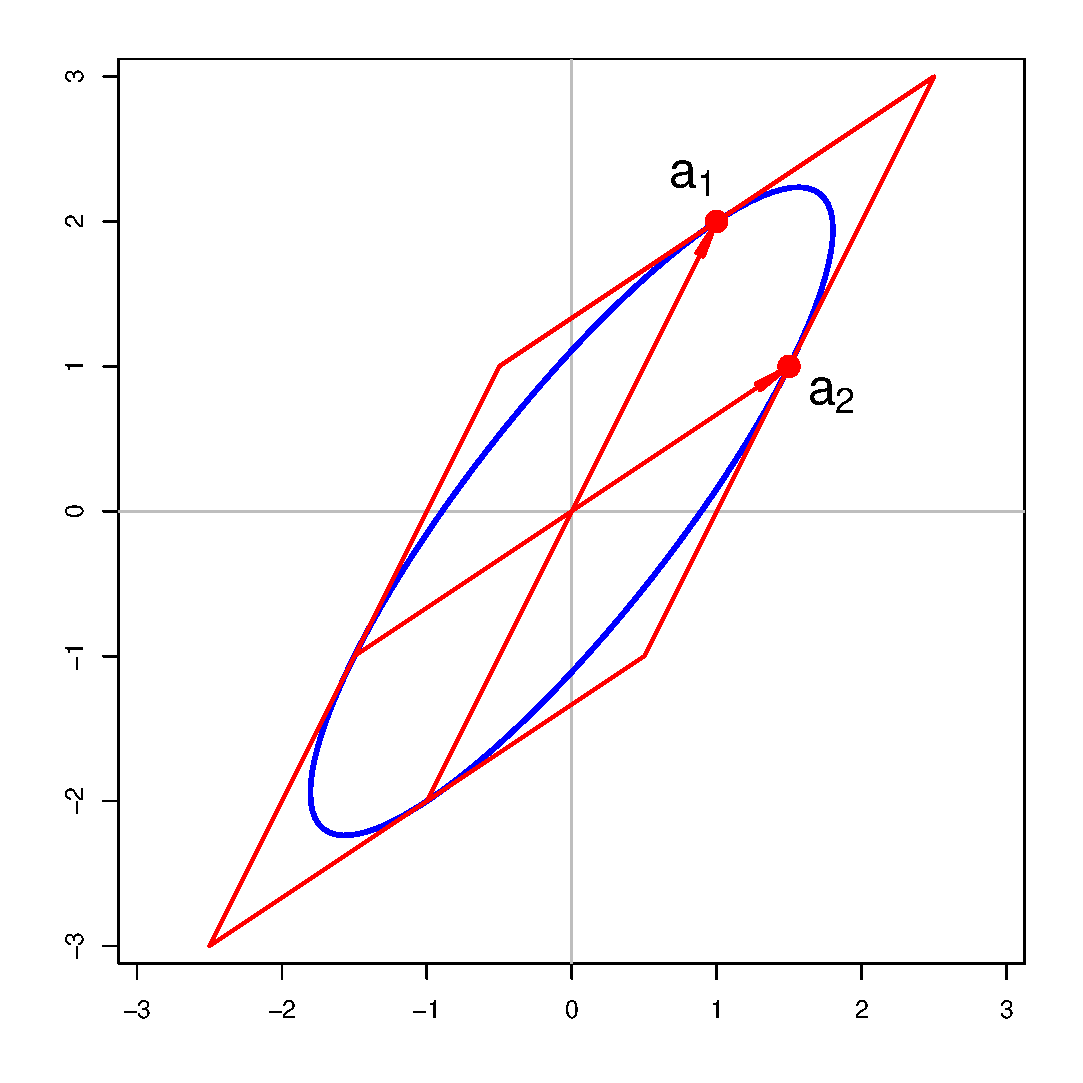
\includegraphics[width=1\linewidth]{fig/conjugate1}
 \end{minipage}%
 \hfill
 \begin{minipage}[b]{.49\linewidth}
  \centering
  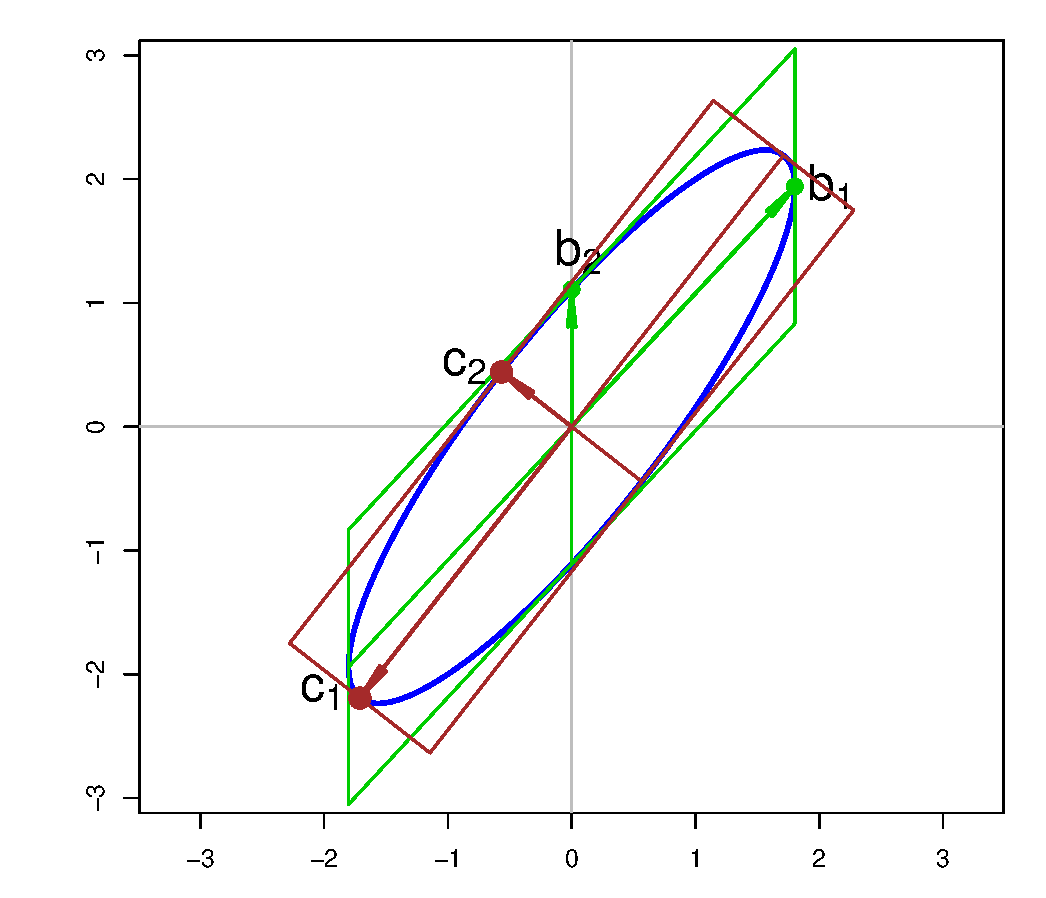
\includegraphics[width=1\linewidth]{fig/conjugate2}
 \end{minipage}
\caption{Conjugate axes of an ellipsoid with various factorizations of $\mat{W}$ and corresponding
basis vectors.
The conjugate vectors lie on the ellipsoid, and their tangents can be extended to form a parallelogram framing it.
Left: for an arbitrary factorization, given in \eqref{eq:fac1}.
Right: for the Choleski factorization (green, $b_1, b_2$) and the principal component factorization (brown, $c_1, c_2$).
}
\label{fig:conjugate}
\end{figure}
For
$p=2$
this result is illustrated in \figref{fig:conjugate} (left)
in which

\begin{equation}\label{eq:fac1}
\mat{A}=\left[ \begin{matrix}
   \vec{a}_{1} & \mat{a}_{2}  \\
\end{matrix} \right]=\left[
\begin{matrix}
   1 & 1.5  \\
   2 & 1  \\
\end{matrix} \right]
\mbox{   }\Rightarrow\mbox{   }
\mat{W}=\mat{A A\trans}=
\left[ \begin{matrix}
   3.25 & 3.5  \\
   3.5 & 5  \\
\end{matrix} \right]
\period
\end{equation}

Consider the inner-product space with inner product matrix 	
$\mat{W}^{-1}=\left[ \begin{matrix}	
1.25 & -0.875 \\	
-0.875 & 0.8125 \\	
\end{matrix} \right]
$ and inner product	
\begin{equation*}
\left\langle \vec{x},\vec{y} \right\rangle =\vec{{x}'W}^{-1}\vec{y} \period
\end{equation*} 	
Because	
$\mat{A}\trans \mat{W}^{-1}\mat{A}
=\mat{A}\trans\left( \mat{A}\mat{A}\trans \right)^{-1}\mat{A}
=\mat{A}\trans(\mat{A}\trans)^{-1}\mat{A}^{-1}\mat{A}
=\mat{I}
$,
we see that
$\vec{a}_{1}$
and	
$\vec{a}_{2}$	
are orthogonal unit vectors (in fact, an orthonormal basis) in this inner product:	

\begin{eqnarray*}
\left\langle \vec{a}_{i},\vec{a}_{i} \right\rangle & = & \vec{{a}\trans}_{i}\mat{W}^{-1}\vec{a}_{i}=1	 \\
%	
\left\langle \vec{a}_{1},\vec{a}_{2} \right\rangle & = &\vec{{a}'}_{1}\mat{W}^{-1}\vec{a}_{2}=0 \period
\end{eqnarray*}


Now, if $\mat{W}=\mat{B{B}\trans}$ is any other factorization of
$\mat{W}$,
then the columns of
$\mat{B}$
have the same properties as the columns of
$\mat{A}$.
Particular factorizations yield interesting and statistically useful sets of conjugate axes.
The illustration in \figref{fig:conjugate} (right) shows two such cases with special properties:
In the Choleski factorization (shown in green), where
$\mat{B}$ is lower triangular, the last conjugate axis, $\vec{b}_2$, is aligned with the coordinate
axis $\vec{x}_2$.  Each previous axis ($\vec{b}_1$, here) is the orthogonal complement to
all later axes in the  inner-product space of
$\mat{W}^{-1}$.  
The Choleski factorization is unique in this respect, subject to a
permutation of the rows and columns of \mat{W}. 
The subspace $\{ c_1 \vec{b}_1 + ... + c_{p-1} \vec{b}_{p-1}  , c_i \in \mathbb{R}\}$, is the plane of the regression of the last variable on the others, a fact that generalizes naturally to ellipsoids that are not necessarily centerered at the origin.  %% added fact /GM  

In the principal-component (PC) factorization (shown in brown) $\mat{W}=\mat{C} \mat{C}\trans$, where
$\mat{C}=\mat{\Gamma \Lambda }^{1/2}$
and hence
$\mat{W}=\mat{\Gamma \Lambda {\Gamma }'}$
is the spectral decomposition of
$\mat{W}$. Here, the ellipse axes are orthogonal in the space of the ellipse
(so the bounding tangent parallelogram is a rectangle) \emph{as well as} in the inner-product space of
$\mat{W}^{-1}$. The PC factorization is unique in this respect (up to reflections of the axis vectors).

As illustrated in \figref{fig:conjugate}, each pair of conjugate axes has a corresponding bounding tangent
parallelogram. It can be shown that all such parallelograms have the same area
and equal sums of squares of the lengths of their diameters.

\subsection{Ellipsoids in a generalized metric space}

%\todo{Georges?}
%\TODO{Smooth out and simplify this description. Add to the plot: unit vectors in data space, and their transformations in canonical space.
%Here it would be useful to describe the geometric relations that pertain to \mat{H}
%(positive semi-definite)
%in the metric of \mat{E} (positive definite).
%I see two sub-figures:
%(a) ellipses for \mat{H} and \mat{E}, showing the conjugate axes and
%bounding parallelogram for \mat{E}, perhaps using the principal component factorization.
%(b) the transformation of (a) using $\mat{H}\mat{E}^{-1}$ or
%$\mat{E}^{-1/2} \, \mat{H} \, \mat{E}^{-1/2}$.
%}

In \secref{sec:conjugate}, we considered the positive semi-definite matrix \mat{W} and
corresponding ellipsoid to be
referred to a Euclidean space, perhaps with different basis vectors.
We showed that various measures of the ``size'' of the ellipsoid could be defined
in terms of functions of the eigenvalues $\lambda_i$ of \mat{W}.

We now consider the generalized
case of an analogous $p \times p$ positive semi-definite symmetric matrix \mat{H}, but where measures of
length, distance, and angles are referred to a metric defined by a positive-definite symmetric
matrix \mat{E}. As is well known, the generalized eigenvalue problem is to find the scalars
$\lambda_i$ and vectors $\vec{v}_i, i=1, 2, \dots p$,
such that $\mat{H} \vec{v} = \lambda \mat{E} \vec{v}$, that is, the roots of
$\det{\mat{H} - \lambda \mat{E}}=0$.

%\TODO{More explanation here ...}
\begin{figure}[htb]
% two figs side-by-side
  \begin{minipage}[c]{.495\textwidth}
   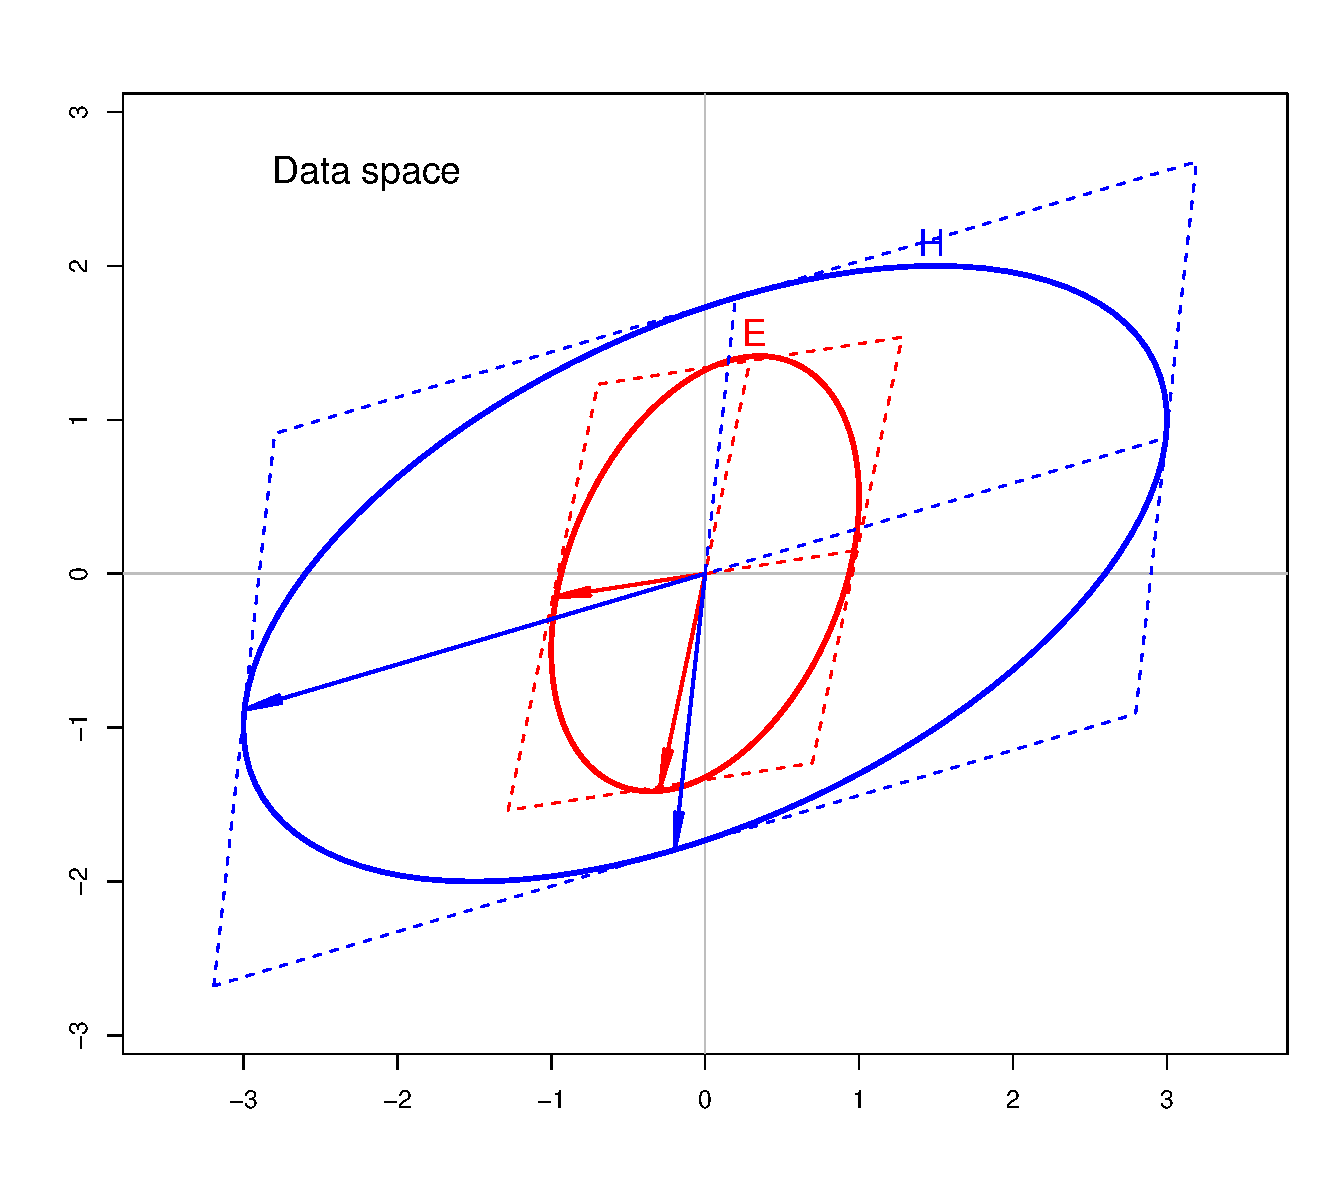
\includegraphics[width=1\linewidth,clip]{fig/ellipse-geneig1}
   \end{minipage}%
  \hfill
  \begin{minipage}[c]{.495\textwidth}
   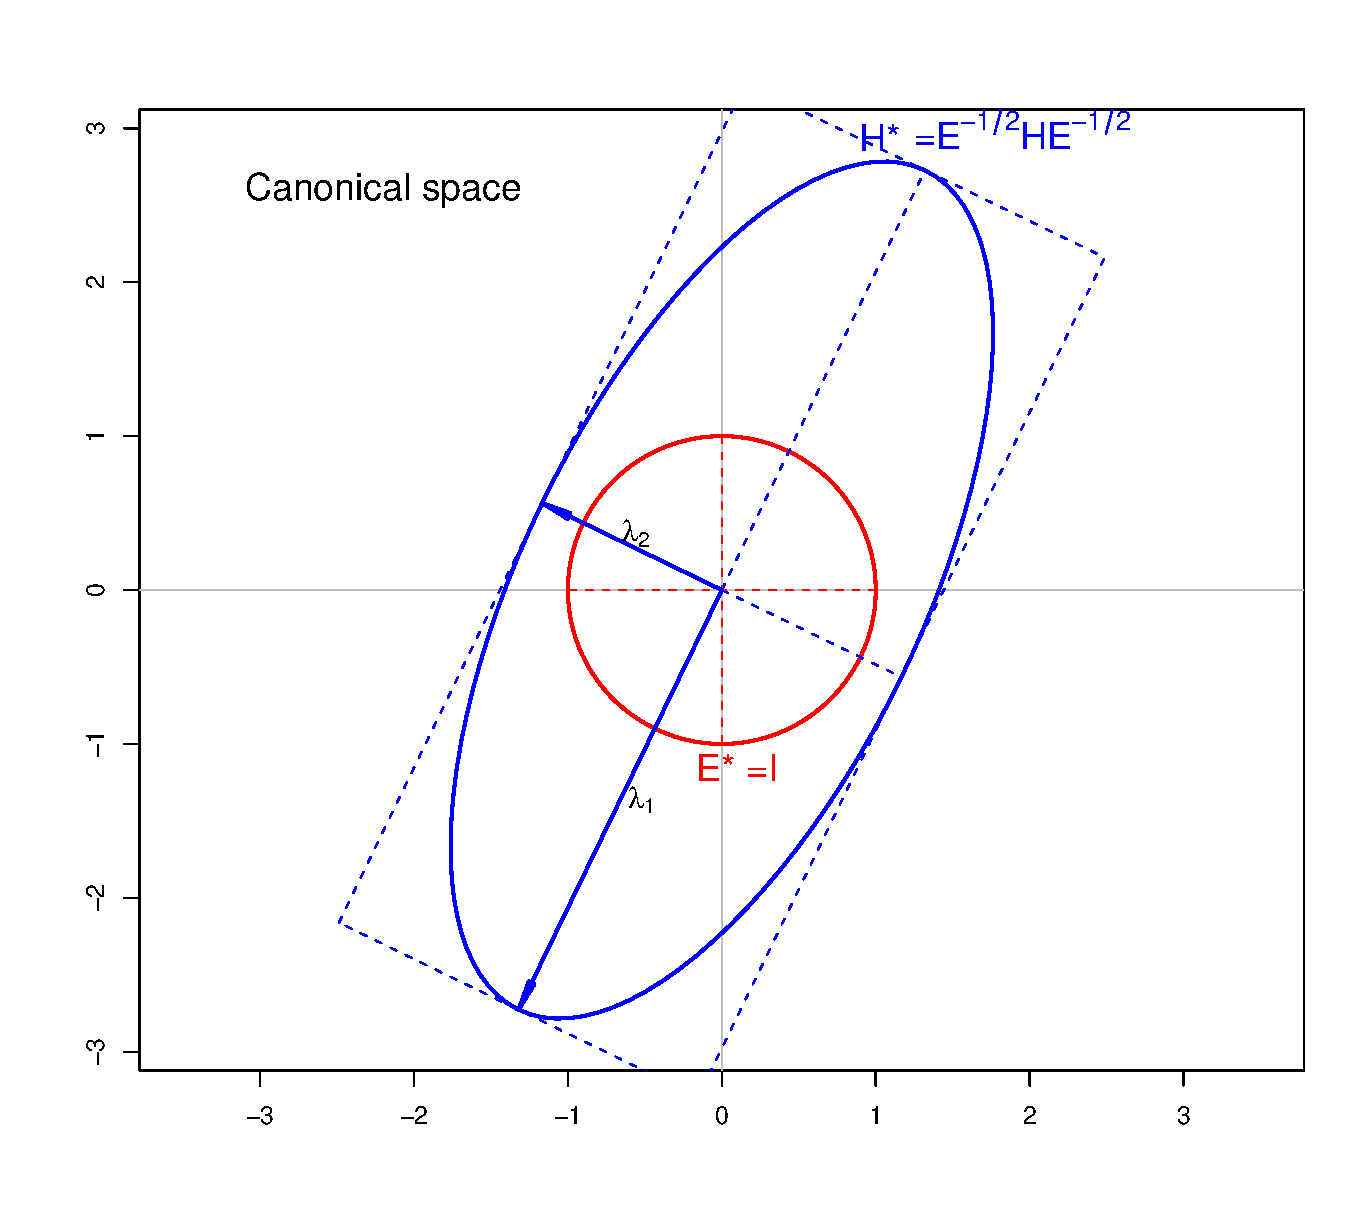
\includegraphics[width=1\linewidth,clip]{fig/ellipse-geneig2}
  \end{minipage}
  \caption{Left: Ellipses for \mat{H} and \mat{E} in Euclidean ``data space,''
   Right: Ellipses for $\mat{H}^\star$ and $\mat{E}^\star$ in the transformed ``canonical space,''
   with the eigenvectors of \mat{H} relative to \mat{E} shown as blue arrows, whose radii
   are the corresponding eigenvalues, $\lambda_1, \lambda_2$. }%
  \label{fig:ellipse-geneig}
\end{figure}
For such \mat{H} and \mat{E}, we can always find a factor \mat{A} of \mat{E}, so that
$\mat{E} = \mat{A} \mat{A}\trans$, whose colums will be conjugate directions for \mat{E}
and whose rows will also be conjugate directions for \mat{H}, in that $\mat{H} = \mat{A}\trans \mat{D} \mat{A}$,
where $\mat{D}$ is diagonal.  Geometrically, this means that there exists a unique pair of
bounding parallelograms for the \mat{H} and \mat{E} ellipsoids whose
corresponding sides are parallel. A linear transformation of \mat{E} and \mat{H}
that transforms the parallelogram
for \mat{E} to a square (or cuboid), and hence \mat{E} to a sphere (or spheroid), generates an
equivalent view in what we describe below as canonical space.


In statistical applications (e.g., MANOVA, canonical correlation), the generalized
eigenvalue problem is transformed to an ordinary eigenvalue problem by considering
the following equivalent forms with the same $\lambda_i$, $\vec{v}_i$,
\begin{eqnarray*}
(\mat{H} - \lambda \mat{E}) \vec{v} & = & \vec{0} \\
\Rightarrow (\mat{H} \, \inv{\mat{E}} - \lambda \mat{I}) \vec{v} & = & \vec{0} \\
\Rightarrow (\invhalf{\mat{E}} \, \mat{H} \, \invhalf{\mat{E}} - \lambda \mat{I}) \vec{v} & = & \vec{0} \comma
\end{eqnarray*}
where the last form gives a symmetric matrix, $\mat{H}^\star = \invhalf{E} \, \mat{H} \, \invhalf{E}$.
Using the square root of \mat{E} defined by the
principal-component factorization $\half{E} = \mat{\Gamma} \half{\mat{\Lambda}}$ produces
the ellipsoid of $\mat{H}^\star$
orthogonal axes corresponding to the $\vec{v}_i$, whose squared radii are the corresponding %% squared / GM
eigenvalues $\lambda_i$.  This can be seen geometrically as a rotation of ``data space''
to an orientation defined by the principal axes of \mat{E}, followed by a re-scaling, so
that the \mat{E} ellipsoid becomes the unit spheroid.  In this transformed space
(``canonical space''), functions of the
the squared radii $\lambda_i$ of the axes of $\mat{H}^\star$ give direct measures of %% squared / GM
the ``size'' of \mat{H} relative to \mat{E}. The orientation of the eigenvectors
$\vec{v}_i$ can be related to the (orthogonal) linear combinations of the
data variables that are successively largest in the metric of \mat{E}.


To illustrate, \figref{fig:ellipse-geneig} (left) shows
the ellipses generated by
\begin{equation*}
 \mat{H} = \left[ \begin{array}{cc}
                   9 & 3 \\
                   3 & 4
                  \end{array}\right]
 \quad \mbox{ and } \quad
 \mat{E} = \left[ \begin{array}{cc}
                   1 & 0.5 \\
                   0.5 & 2
                  \end{array}\right]
\end{equation*}
together with their conjugate axes. For \mat{E}, the conjugate axes are defined by the columns of the right factor,
$\mat{A}\trans$,
in $\mat{E} = \mat{A} \mat{A}\trans$; for \mat{H}, the conjugate axes are defined by the columns of $\mat{A}$.
The transformation to $\mat{H}^\star = \invhalf{E} \, \mat{H} \, \invhalf{E}$ is shown in the right panel
of \figref{fig:ellipse-geneig}. In this ``canonical space,'' angles and lengths have the orginary interpretation
of Euclidean space, so the size of $\mat{H}^\star$ can be interpreted directly in terms of functions of
the radii $\sqrt{\lambda_1}$ and $\sqrt{\lambda_2}$.


%\section{The data ellipse and ellipsoids}\label{sec:data-ellipse}

The \emph{data ellipse} \citep{Monette:90} (or \emph{concentration ellipse}, \citealp[Ch. 7]{Dempster:69})
provides a remarkably
simple and effective display for viewing and understanding
bivariate \emph{marginal} relationships in multivariate data.
The data ellipse is typically used to add a visual summary to a scatterplot,
indicating the means, standard deviations, correlation,
and slope of the regression line for
two variables. Under classical (Gaussian) assumptions, the data ellipse
provides a statistically sufficient visual summary, as we describe below.


\begin{figure}[htb]
  \centering
  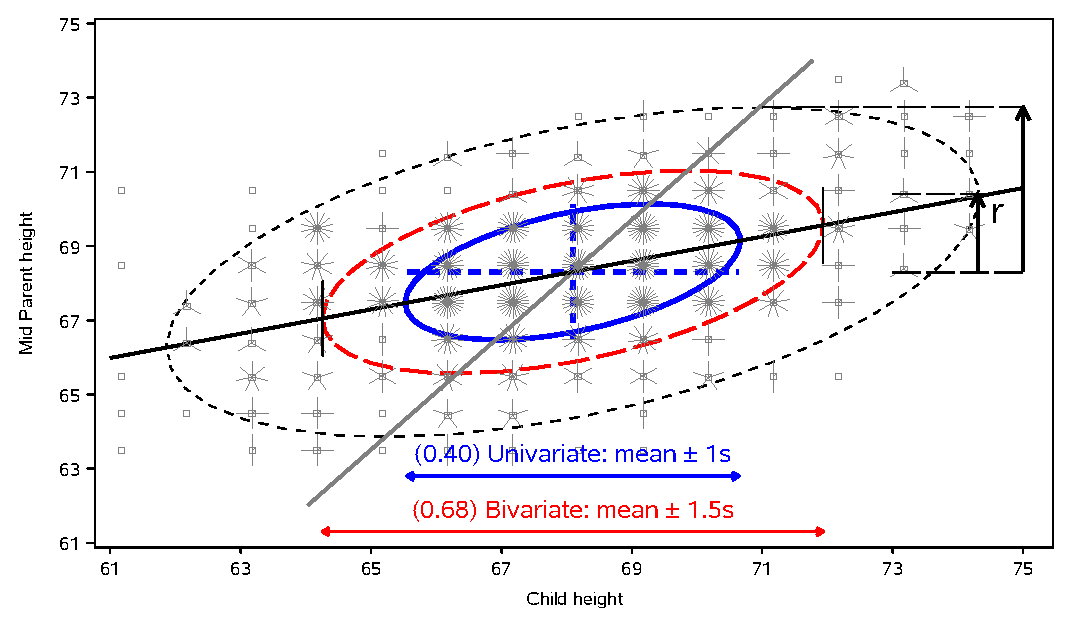
\includegraphics[width=.9\textwidth,clip]{fig/galton-reg3}
  \caption{Sunflower plot of Galton's data on heights of parents and their children (in.), with
  40\%, 68\% and 95\% data ellipses and the regression lines of $y$ on $x$ (black) and
  $x$ on $y$ (grey). The ratio of the vertical to the regression line (labeled `r') to the vertical
  to the top of the ellipse gives a visual estimate of the correlation ($r$=0.46, here).
  Shadows (projections) on the coordinate axes give standard intervals, 
  $\bar{x} \pm k s_x$ and $\bar{y} \pm k s_y$, 
  with $k=1, 1.5, 2.45$, having
  bivariate coverage 40\%, 68\% and 95\%, and univariate coverage 68\%, 87\% and 98.6\% respectively.
%with various coverage properties.
  Plotting children's height on the abscissa follows Galton.
  }%
  \label{fig:galton-reg3}
\end{figure}

It is historically appropriate to illustrate the data ellipse and
describe its properties using Galton's (\citeyear[Table
I]{Galton:1886})
data, from which he drew \figref{fig:galton-corr} as a conceptual
diagram,%
\footnote{These data are reproduced in \citet[Table 8.2, p.
286]{Stigler:1986}}
shown in \figref{fig:galton-reg3}, where the frequency at
each point is represented by a sunflower symbol. We also overlay the 40\%,
68\% and 95\% data ellipses, as described below.

In \figref{fig:galton-reg3}, the ellipses have the mean vector
$(\bar{x}, \bar{y})$ as their center;  the lengths of arms of the
central cross show the standard deviations of the variables, which
correspond to the shadows of the 40\% ellipse.  In
addition, the correlation coefficient can be visually represented as
the fraction of a vertical tangent line from $\bar{y}$ to the top of
the ellipse that is below the regression line $\widehat{y} | x$, shown
by the arrow labeled `r.' Finally, as Galton noted, the regression line
for $\widehat{y} \given x$ (or $\widehat{x} \given y$)
can be visually estimated as the locus of the points of vertical
(or horizontal) tangents with the family of concentric ellipses.
See \citet[Figs.~5.1--5.2]{Monette:90} and
\citet[p.~183]{Friendly:91} for illustrations and further discussion
of the properties of the data ellipse.

More formally \citep{Dempster:69,Monette:90}, for a $p$-dimensional
sample, $\mat{Y}_{n \times p}$,
we recognize the quadratic form in \eqref{eq:ellipsoid3}
as corresponding to the squared Mahalanobis distance,
$D^2_M (\vec{y}) = \dev{\vec{y}}\trans \, \inv{S} \, \dev{\vec{y}}$,
of the point
$\vec{y} = (y_1, y_2, \dots , y_p)\trans$
from the centroid of the sample,
$\bar{\vec{y}} = (\bar{y}_1, \bar{y}_2, \dots , \bar{y}_p)\trans$.
Thus, we use a more explicit notation to
define the \emph{data ellipsoid} $\mathcal{E}_c$ of size (``radius'') $c$
as the set of all points $\vec{y}$ with $D^2_M (\vec{y})$ less than or
equal to $c^2$,
\begin{equation}\label{eq:dsq}
\mathcal{E}_c ( \bar{\vec{y}},  \mat{S} )
:= \{ \vec{y} :
\dev{\vec{y}}\trans \, \inv{S} \, \dev{\vec{y}} \le c^2 \} \comma
\end{equation}
where
$\mat{S} = ({n-1})^{-1} \sum_{i=1}^n (\vec{y}_i - \bar{\vec{y}}) (\vec{y}_i - \bar{\vec{y}}\trans)$
is the sample covariance matrix.  In the computational notation of \eqref{eq:ellipsoidW}, the boundary of the
data ellipsoid of radius $c$ is thus
\begin{equation}\label{eq:ellipsoidS}
\mathcal{E}_c(\bar{\vec{y}}, \mat{S}) = \bar{\vec{y}} \oplus c \mat{S}^{1/2} \period
\end{equation}

Many properties of the data ellipsoid hold regardless of the joint distribution of the
variables; but if the variables are multivariate normal, then the data ellipsoid approximates
a contour of constant density in their joint distribution.  In this case $D^2_M (x,y)$
has a large-sample $\chi^2_p$ distribution, or, in finite samples, approximately
$[p (n-1) / (n-p)] F_{p, n-p}$).

Hence, in the bivariate case, taking $c^2 = \chi^2_2(0.95)= 5.99 \approx 6$ encloses approximately
95\% of the data points under normal theory.  Other radii also have useful interpretations:
\begin{itemize*}
\item In \figref{fig:galton-reg3}, we demonstrate that $c^2 = \chi^2_2(0.40) \approx 1$ gives
a data ellipse of 40\% coverage with the property that its projection on either axis
corresponds to a standard interval, $\bar{x} \pm 1 s_x$ and $\bar{y} \pm 1 s_y$.  The same property of univariate
coverage pertains to
any linear combination of $x$ and $y$.
\item By analogy with a univariate sample, a 68\% coverage data ellipse with
$c^2 = \chi^2_2(0.68) = 2.28$ gives a bivariate analog of the standard $\bar{x} \pm 1 s_x$ and $\bar{y} \pm 1 s_y$ intervals.
The univariate shadows, or those of any linear combination, then correspond to standard Scheff\'e
intervals taking ``fishing'' (simultaneous interfence) in a $p=2$-dimensional space into account.
\end{itemize*}


\begin{figure}[htb]
% two figs side-by-side
  \begin{minipage}[c]{.485\textwidth}
   \includegraphics[width=1\linewidth,clip]{fig/scatirisd1}
   \end{minipage}%
  \hfill
  \begin{minipage}[c]{.485\textwidth}
   \includegraphics[width=1\linewidth,clip]{fig/scatirisd3}
  \end{minipage}
  \caption{Scatterplot matrices of Anderson's iris data: (a) showing data, separate 68\% data
  ellipses, and regression lines for each species; (b) showing only ellipses and regression lines.
  Key-- \emph{Iris setosa}: blue, $\triangle$; \emph{Iris versicolor}: red, $+$;
  \emph{Iris virginca}: green, $\Box$.}%
  \label{fig:scatirisd1}
\end{figure}

As useful as the data ellipse might be for a single, unstructured
sample, its value as a visual summary increases
with the complexity of the data.
For example, \figref{fig:scatirisd1} shows  scatterplot matrices
of all pairwise plots of the variables from Edgar Anderson's \citeyear{Anderson:35}
classic
data on three species of iris flowers found in the Gasp\'{e} Peninsula,
later used by \citet{Fisher:36} in his development of discriminant analysis.
The data ellipses show clearly that the means, variances, correlations,
and regression slopes differ systematically across the three iris species
in all pairwise plots.
We emphasize that the ellipses serve as sufficient visual summaries of the important
statistical properties (first and second moments)% 
\footnote{
We recognize that a normal-theory summary (first and second moments),
shown visually or numerically, can be distorted
by multivariate outliers, particularly in smaller samples.
In what follows,
robust covariance estimates can, in principle, be substituted
for the classical, normal-theory estimates in all cases.
% Such effects can be countered by using
% robust covariance
% estimates such as multivariate trimming \citep{GnanadesikanKettenring:72}
% or the high-breakdown bound Minimum Volume Ellipsoid (MVE) and
% Minimum Covariance Determinant (MCD) methods
% developed by Rousseeuw and others
% \citep{RousseeuwLeroy:87,RousseeuwVanDriessen:99}.
% In what follows, it should be noted that
% robust covariance estimates could, in principle, be substituted
% for the classical, normal-theory estimates in all cases.
To save space, we don't explore these possibilities further here.
}
by removing the data points
from the plots in the version at the right.

%\subsection{Robust data ellipsoids}




\section{Linear models: data ellipses and confidence ellipses}

Here we consider how ellipses help to visualize relationships among variables
in connection with linear models (regression, ANOVA).
We begin with views in the space of the variables (data space)
and progress to related views in the space of model parameters
($\vec{\beta}$ space).

\subsection{Simple linear regression}

Various aspects of the standard data ellipse of radius 1 illuminate many properties
of simple linear regression, as shown in \figref{fig:ellipses-demo}.
These properties are also useful in more complex contexts.

\begin{figure}[htb]
  \centering
  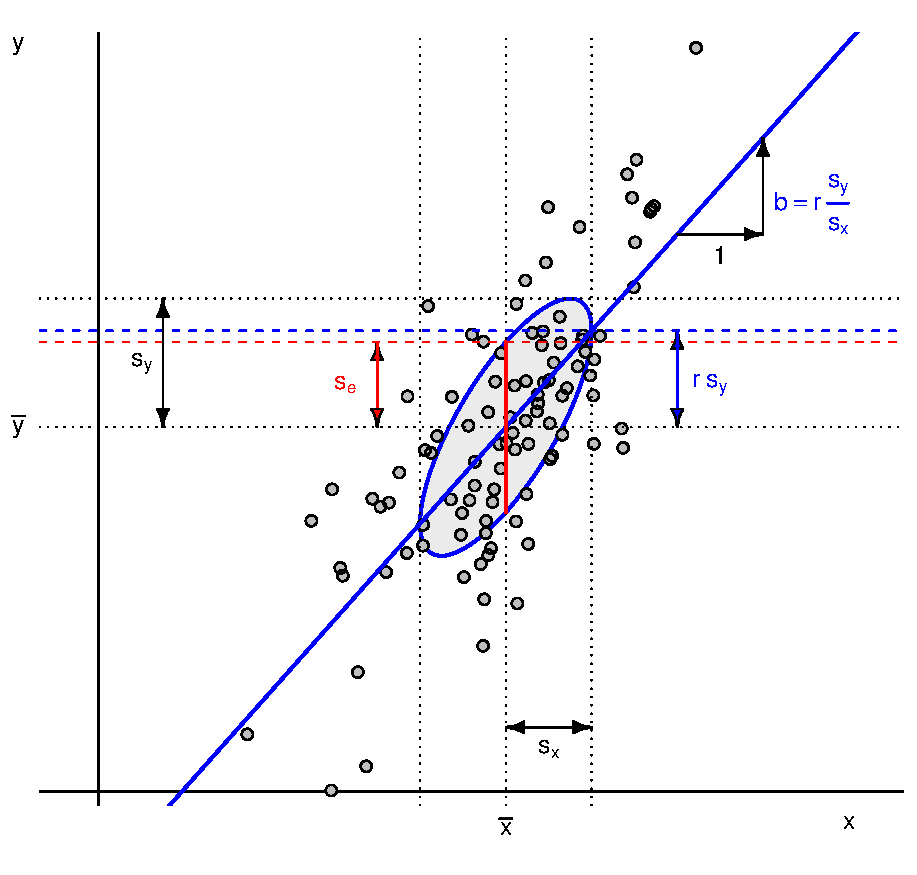
\includegraphics[width=.6\textwidth,clip]{fig/ellipses-demo}
  \caption{Annotated standard data ellipse showing standard deviations of $x$ and $y$, residual
  standard deviation ($s_e$), slope ($b$), and correlation ($r$).
  }%
  \label{fig:ellipses-demo}
\end{figure}

\begin{itemize}
  \item One-half of the widths of the vertical and horizontal projections (dotted black lines)
  give the standard deviations $s_x$ and $s_y$ respectively.
  \item Since any line through the center of the ellipse ($\bar{x}, \bar{y}$), corresponds to
  some linear combination, $m x + n y$, the half-width of the corresponding tangent lines
  gives the standard deviation of this linear combination.
  \item The standard deviation of the residuals, $s_e$ may be seen as the half-width of the vertical
  (red) line at $x=\bar{x}$.
  \item The vertical distance between the mean of $y$ and the points where the ellipse has vertical
  tangents is $r s_y$. (As a fraction of $s_y$, this distance is $r = 0.75$ in the figure.)
  \item The (blue) regression line of $y$ on $x$ passes through the points of vertical tangency.
  Similarly, the regression of $x$ on $y$ (not shown) passes through the points of
  horizontal tangency.
  
\end{itemize}

\subsection{Visualizing a confidence interval for the slope}
A visual approximation to a 95\% confidence interval for the slope, and thus a visual test of $H_0 : \beta = 0$
may be seen in \figref{vis-reg-prestige}.  From the formula for a 95\% confidence interval,
$CI_{.95} (\beta) = b \pm t_{n-2}^{0.975} \times SE(b)$, we can take $t_{n-2}^{0.975} \approx 2$
and 
 $SE(b) \approx \frac{1}{\sqrt{n}}\left( \frac{s_e}{s_x} \right)$, 
leading to
\begin{equation}\label{eq:ci-approx}
CI_{.95} (\beta) \approx b \pm \frac{2}{\sqrt{n}} \times \left( \frac{s_e}{s_x} \right) \period
\end{equation}
%\todo{fix the notation in these figures}
\begin{figure}[htb]
% two figs side-by-side
  \begin{minipage}[c]{.49\textwidth}
   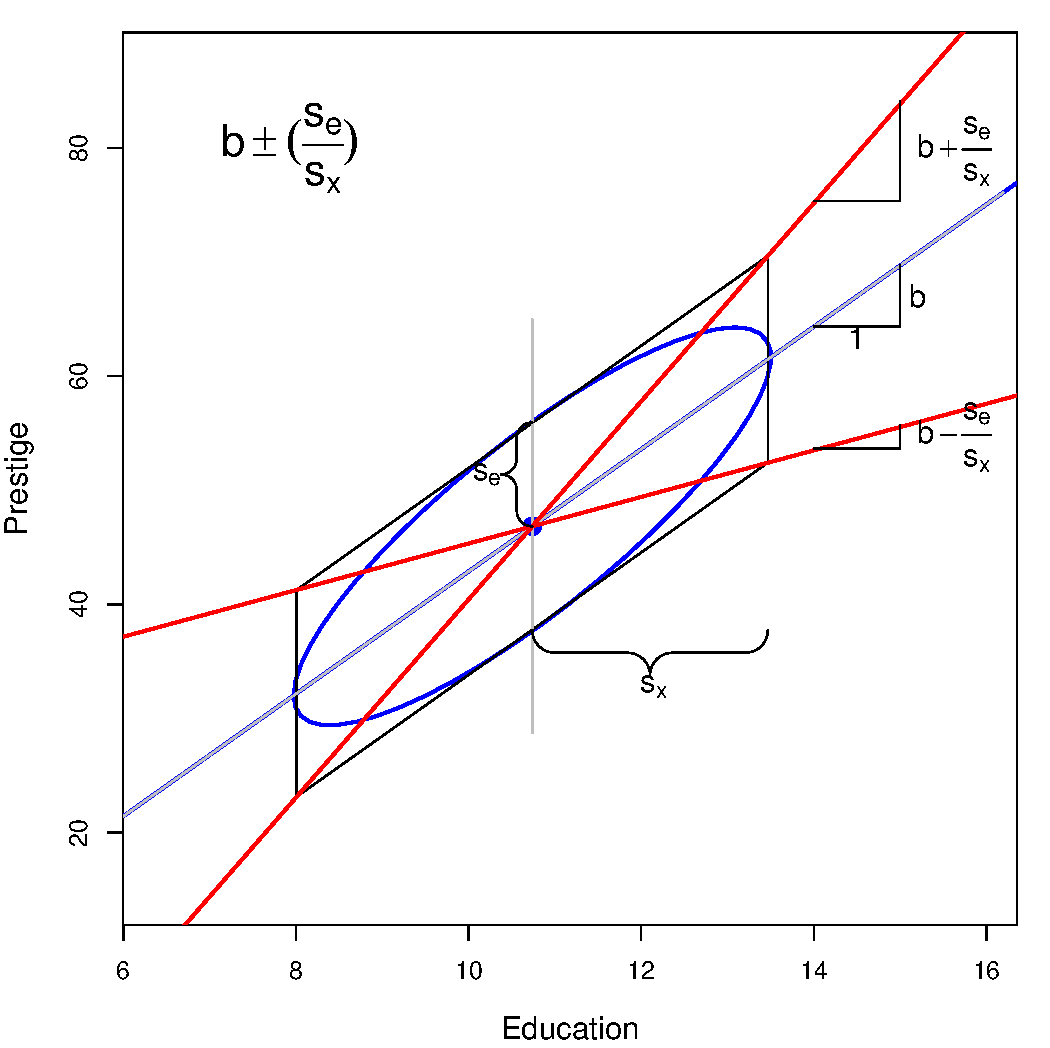
\includegraphics[width=1\linewidth,clip]{fig/vis-reg-prestige1}
   \end{minipage}%
  \hfill
  \begin{minipage}[c]{.49\textwidth}
   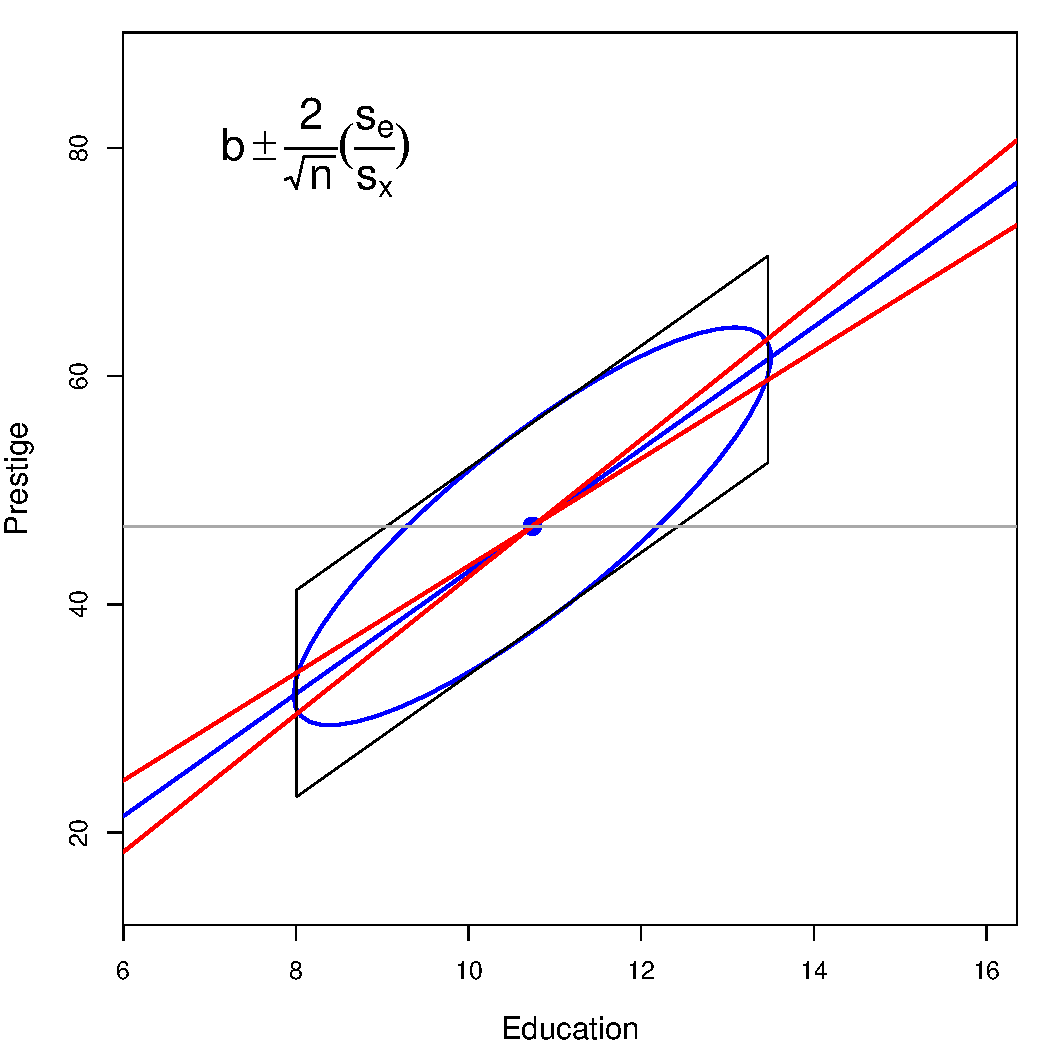
\includegraphics[width=1\linewidth,clip]{fig/vis-reg-prestige2}
  \end{minipage}
  \caption{Visual 95\% confidence interval for the slope in linear regression. Left: Standard data ellipse surrounded by the 
  regression parallelogram. Right: Shrinking the diagonal lines by a factor of $2/\sqrt{n}$,
  giving the approximate 95\% confidence interval for $\beta$.}%
  \label{vis-reg-prestige}
\end{figure}

To show this visually, the left panel of \figref{vis-reg-prestige} shows the standard data ellipse
surrounded by the ``regression parallelogram'', formed with the vertical tangent lines and the
tangent lines parallel to the regression line. This corresponds to the conjugate axes of the
ellipse induced by the Choleski factor of $S_{yx}$ as shown in \figref{fig:conjugate}.
Simple algebra shows that the diagonal lines through
this parallelogram have slopes of
\begin{equation*}
 b \pm \frac{s_{e}}{s_x}
\end{equation*}
So, to obtain a visual estimate of the 95\% confidence interval, we need only shrink the diagonal lines of the
regression parallelogram toward the regression line by a factor of $2/\sqrt{n}$, giving the red lines
in the right panel of \figref{vis-reg-prestige}.  
In the data used for this
example, $n=102$, so the factor  is approximately 0.2 here.
Now consider the horizontal line through the center of the data ellipse.  If this line is outside the 
envelope of the confidence lines, we can reject $H_0 : \beta = 0$ via this simple visual approximation.

\subsection{Simpson's paradox, marginal and conditional relationships}\label{sec:simpson-iris}

Because it provides a visual summary of means, variances, and correlations,
the data ellipse is ideally suited as a tool for illustrating and
explicating various
phenomena that occur in the analysis of linear models.
One class of simple, but important, examples concerns the difference between the marginal
relationship between variables, ignoring some important factor or covariate,
and the conditional relationship, adjusting (controlling) for that
factor or covariate.

\begin{figure}[htb]
  \centering
  \includegraphics[width=\textwidth,clip]{fig/contiris3}
  \caption{Marginal (a), conditional (b), and pooled within-sample (c) relationships
  of Sepal length and Sepal width in the iris data. Total-sample data ellipses are
  shown as black, solid curves; individual-group data and ellipses are shown with
  colors and dashed lines}%
  \label{fig:contiris3}
\end{figure}

Simpson's paradox \citep{Simpson:51} occurs when the marginal and
conditional relationships differ in direction. This may be seen in the plots
of Sepal length and Sepal width for the iris data shown in \figref{fig:contiris3}. Ignoring
iris species, the marginal, total-sample correlation is slightly negative
as seen in panel (a). The individual-sample ellipses in panel (b) show
that the conditional, within-species correlations are all positive, with
approximately equal regression slopes.  The group means have a negative
relationship, accounting for the negative marginal correlation.

A correct analysis of the (conditional) relationship between these variables, controlling or adjusting for mean
differences among species, is based on the pooled within-sample covariance matrix,
  \begin{equation} \label{eq:Sp}
  \mat{S}_{\textrm{within}}  = (N - g)^{-1}
  \sum_{i=1}^g
  \sum_{j=1}^{n_i}
  ( \vec{y}_{ij}  -  \bar{\vec{y}}_{i.} )
  ( \vec{y}_{ij}  -  \bar{\vec{y}}_{i.} ) \trans
  =(N - g)^{-1}
  \sum_{i=1}^g
  (n_i - 1) \mat{S}_i
  \comma
  \end{equation}
where $N = \sum n_i$, and the result
is shown in
panel (c) of \figref{fig:contiris3}.
In this graph, the data for \emph{each} species were first
transformed to deviations from the species means on both variables
and then translated back to the grand means.

In a more general context, $ \mat{S}_{\textrm{within}}$
appears as the $\mat{E}$ matrix in a multivariate
linear model, adjusting or controlling for all fitted effects (factors and covariates).
For essentially correlational analyses (principal components,
factor analysis, etc.),
similar displays can be used to show how multi-sample analyses
can be compromised by substantial group mean differences, and corrected
by analysis of the pooled within-sample covariance matrix, or by
including important group variables in the model.
Moreover, display of the the individual within-group data ellipses can
show visually how well the assumption of
equal covariance matrices,
$\Sigma_1 = \Sigma_2 = \dots = \Sigma_g$,
is satisfied in the data, for the two variables
displayed.


\subsection{Other paradoxes and fallacies}

Data ellipses can also be used to visualize and understand other paradoxes and
fallacies that occur with linear models.  We consider situations in which there
is a principal relationship between variables $y$ and $x$ of interest, but (as in the preceding subsection) the data
are stratified in $g$  samples by a factor (``group'') that might correspond
to different subpopulations (e.g., men and women, age groups),
different spatial regions (e.g., states), different points in time, or some
combination of the above.

In some cases, group may be unknown, or may not have been included in the model,
so we can only estimate the marginal association between $y$ and $x$,
giving a slope $\beta_{\textrm{marginal}}$ and correlation $r_{\textrm{marginal}}$.
In other cases, we may not have individual data, but only aggregate group
data, $(\bar{y}_i, \bar{x}_i), i=1, \dots , g$, from which we can estimate
the between-groups (``ecological'') association, with slope
$\beta_{\textrm{between}}$ and correlation $r_{\textrm{between}}$.
When all data are available and the model is an ANCOVA model of the form
$y \sim x + \textrm{group}$,
we can estimate a common conditional, within-group slope,
$\beta_{\textrm{within}}$, or, with the model $y \sim x + x \times \textrm{group}$,
the separate within-group slopes, $\beta_i$.


\begin{figure}[htb]
 \begin{minipage}[b]{.49\linewidth}
  \centering
  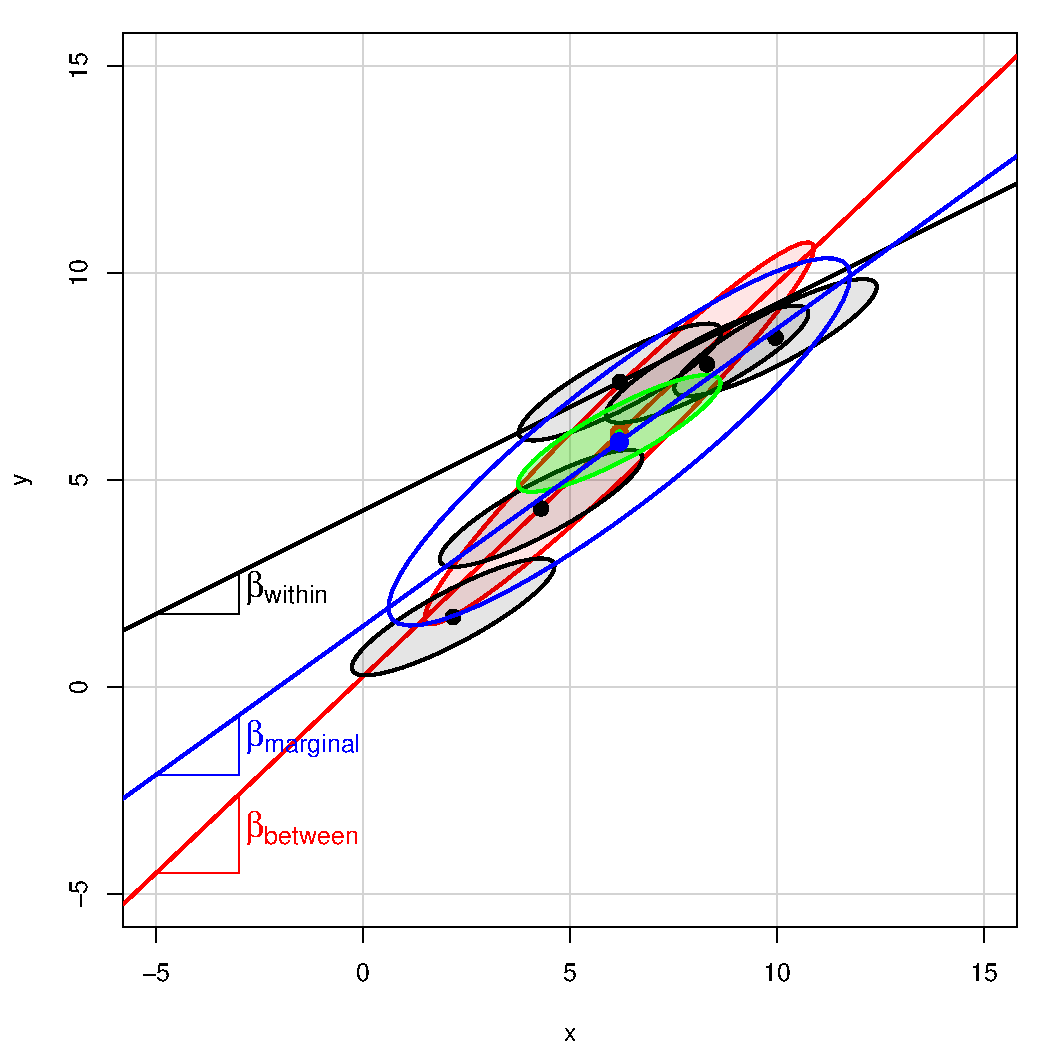
\includegraphics[width=1\linewidth]{fig/between-within1}
 \end{minipage}%
 \hfill
 \begin{minipage}[b]{.49\linewidth}
  \centering
  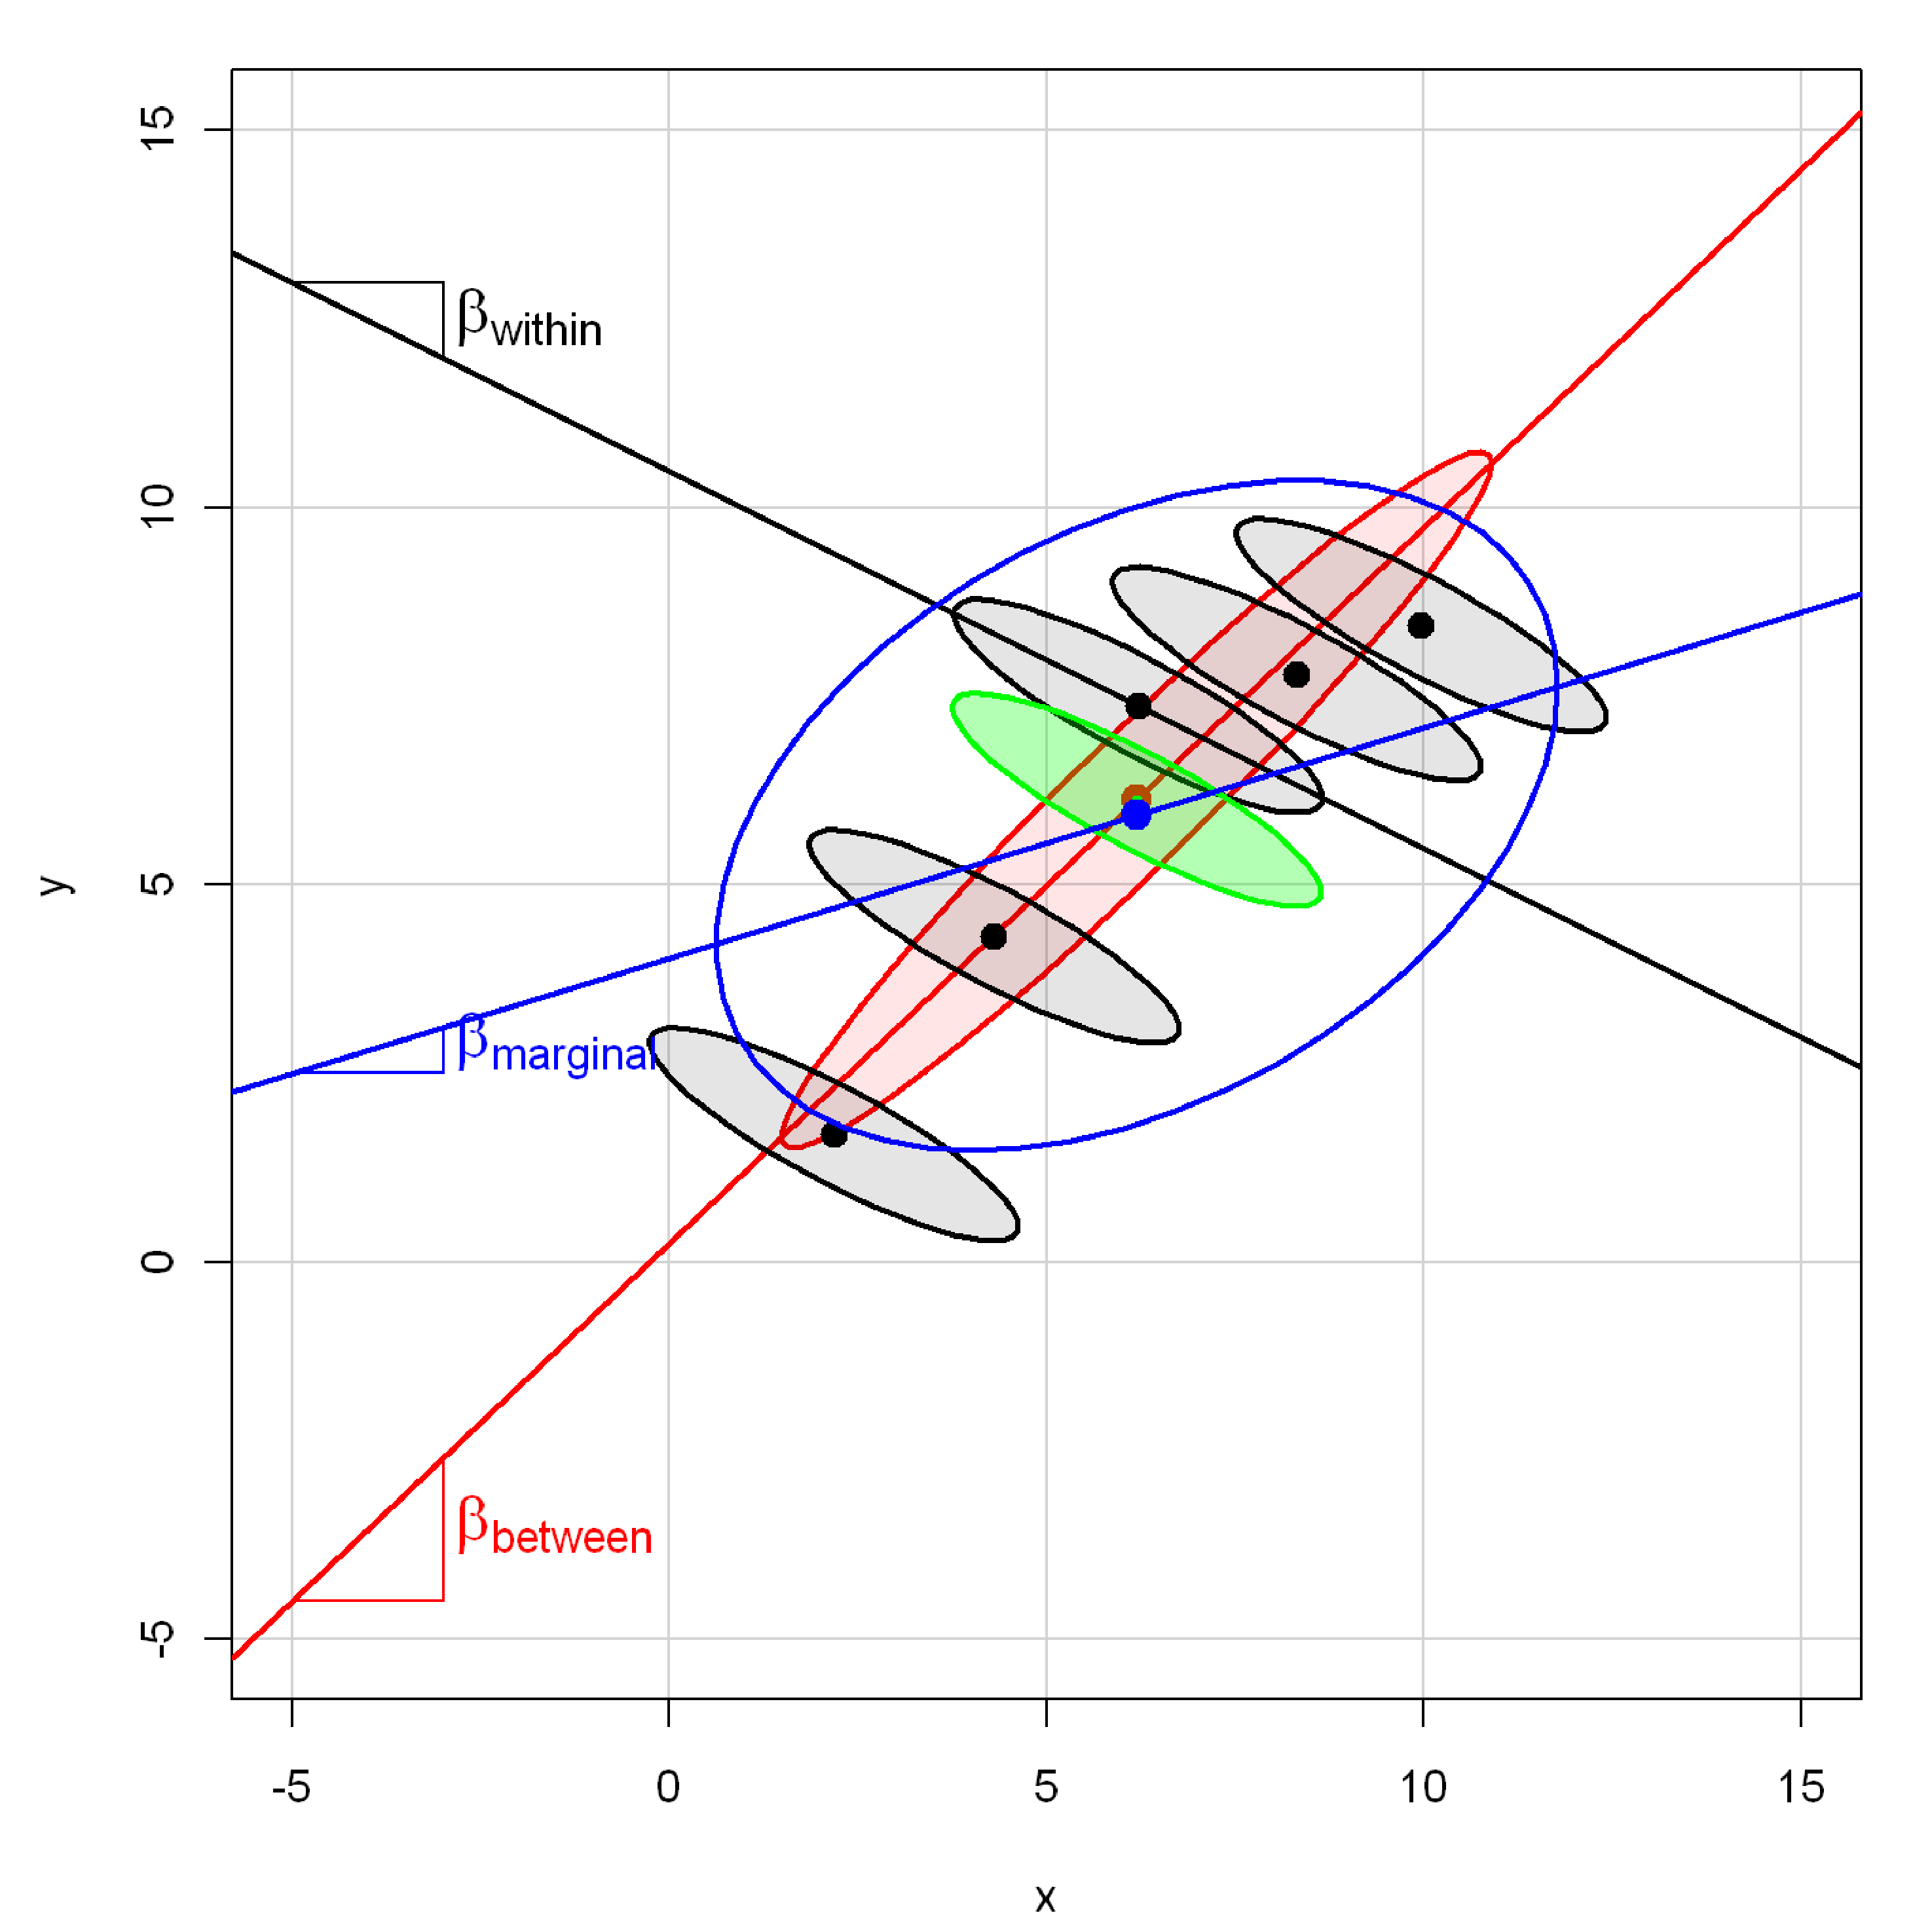
\includegraphics[width=1\linewidth]{fig/between-within2}
 \end{minipage}
  \caption{Paradoxes and fallacies: between (ecological), within (conditional) and whole-sample (marginal) associations.
  In both panels, the five groups have the same group means, and $\Var(x)=6$ and $\Var(y)=2$ within each group.
  The within-group correlation is $r = +0.87$ in all groups in the left panel, and is $r = -0.87$ in the right panel.
  The green ellipse shows the average within-group data ellipse.}
  \label{fig:between-within}
\end{figure}

\figref{fig:between-within} illustrates these estimates in a simulation of five groups, with $n_i=10$,  means
$\bar{x}_i = 2 \, i + \mathcal{U}(-0.4, 0.4)$  and
$\bar{y}_i = \bar{x}_i + \mathcal{N}(0, 0.5)$, so that $r_{\textrm{between}} \approx 0.95$.
For simplicity, we have set the within-group covariance matrices to be identical in all groups, with
$\Var(x)=6$, $\Var(y)=2$ ,and $\Cov(x,y)=\pm 3$ in the left and right panels, respectively, giving
$r_{\textrm{within}} = \pm 0.87$.

In the left panel, the conditional, within-group slope is smaller than the ecological, between-group slope,
reflecting the smaller within-group than between-group correlation.
In general, however, it can be shown that
\begin{equation*}
\vec{\beta}_{\textrm{marginal}} \in [\vec{\beta}_{\textrm{within}} , \vec{\beta}_{\textrm{between}} ] \comma
\end{equation*}
which is also evident in the right panel, where the within-group slope is negative.
This result follows from the fact that the marginal data ellipse for the total sample
has a shape that is a convex combination (weighted average) of the average within-group
covariance of $(x, y)$, shown by the green ellipse in  \figref{fig:between-within},
and the  covariance of the means $(\bar{x}_i, \bar{y}_i)$, shown by the red between-group ellipse.
In fact, the between and within data ellipses in  \figref{fig:between-within}
are just (a scaling of) the $\mat{H}$ and $\mat{E}$ ellipses in an hypothesis-error (HE) plot for the
MANOVA model, $(x, y) \sim \textrm{group}$, as will be developed in \secref{sec:mlm}.
See \figref{fig:between-HE} for a visual demonstration, using the same data  as in   \figref{fig:between-within}.
%\TODO{Can we show this analytically in some insightful way?}

\begin{figure}[htb]
 \begin{minipage}[b]{.49\linewidth}
  \centering
  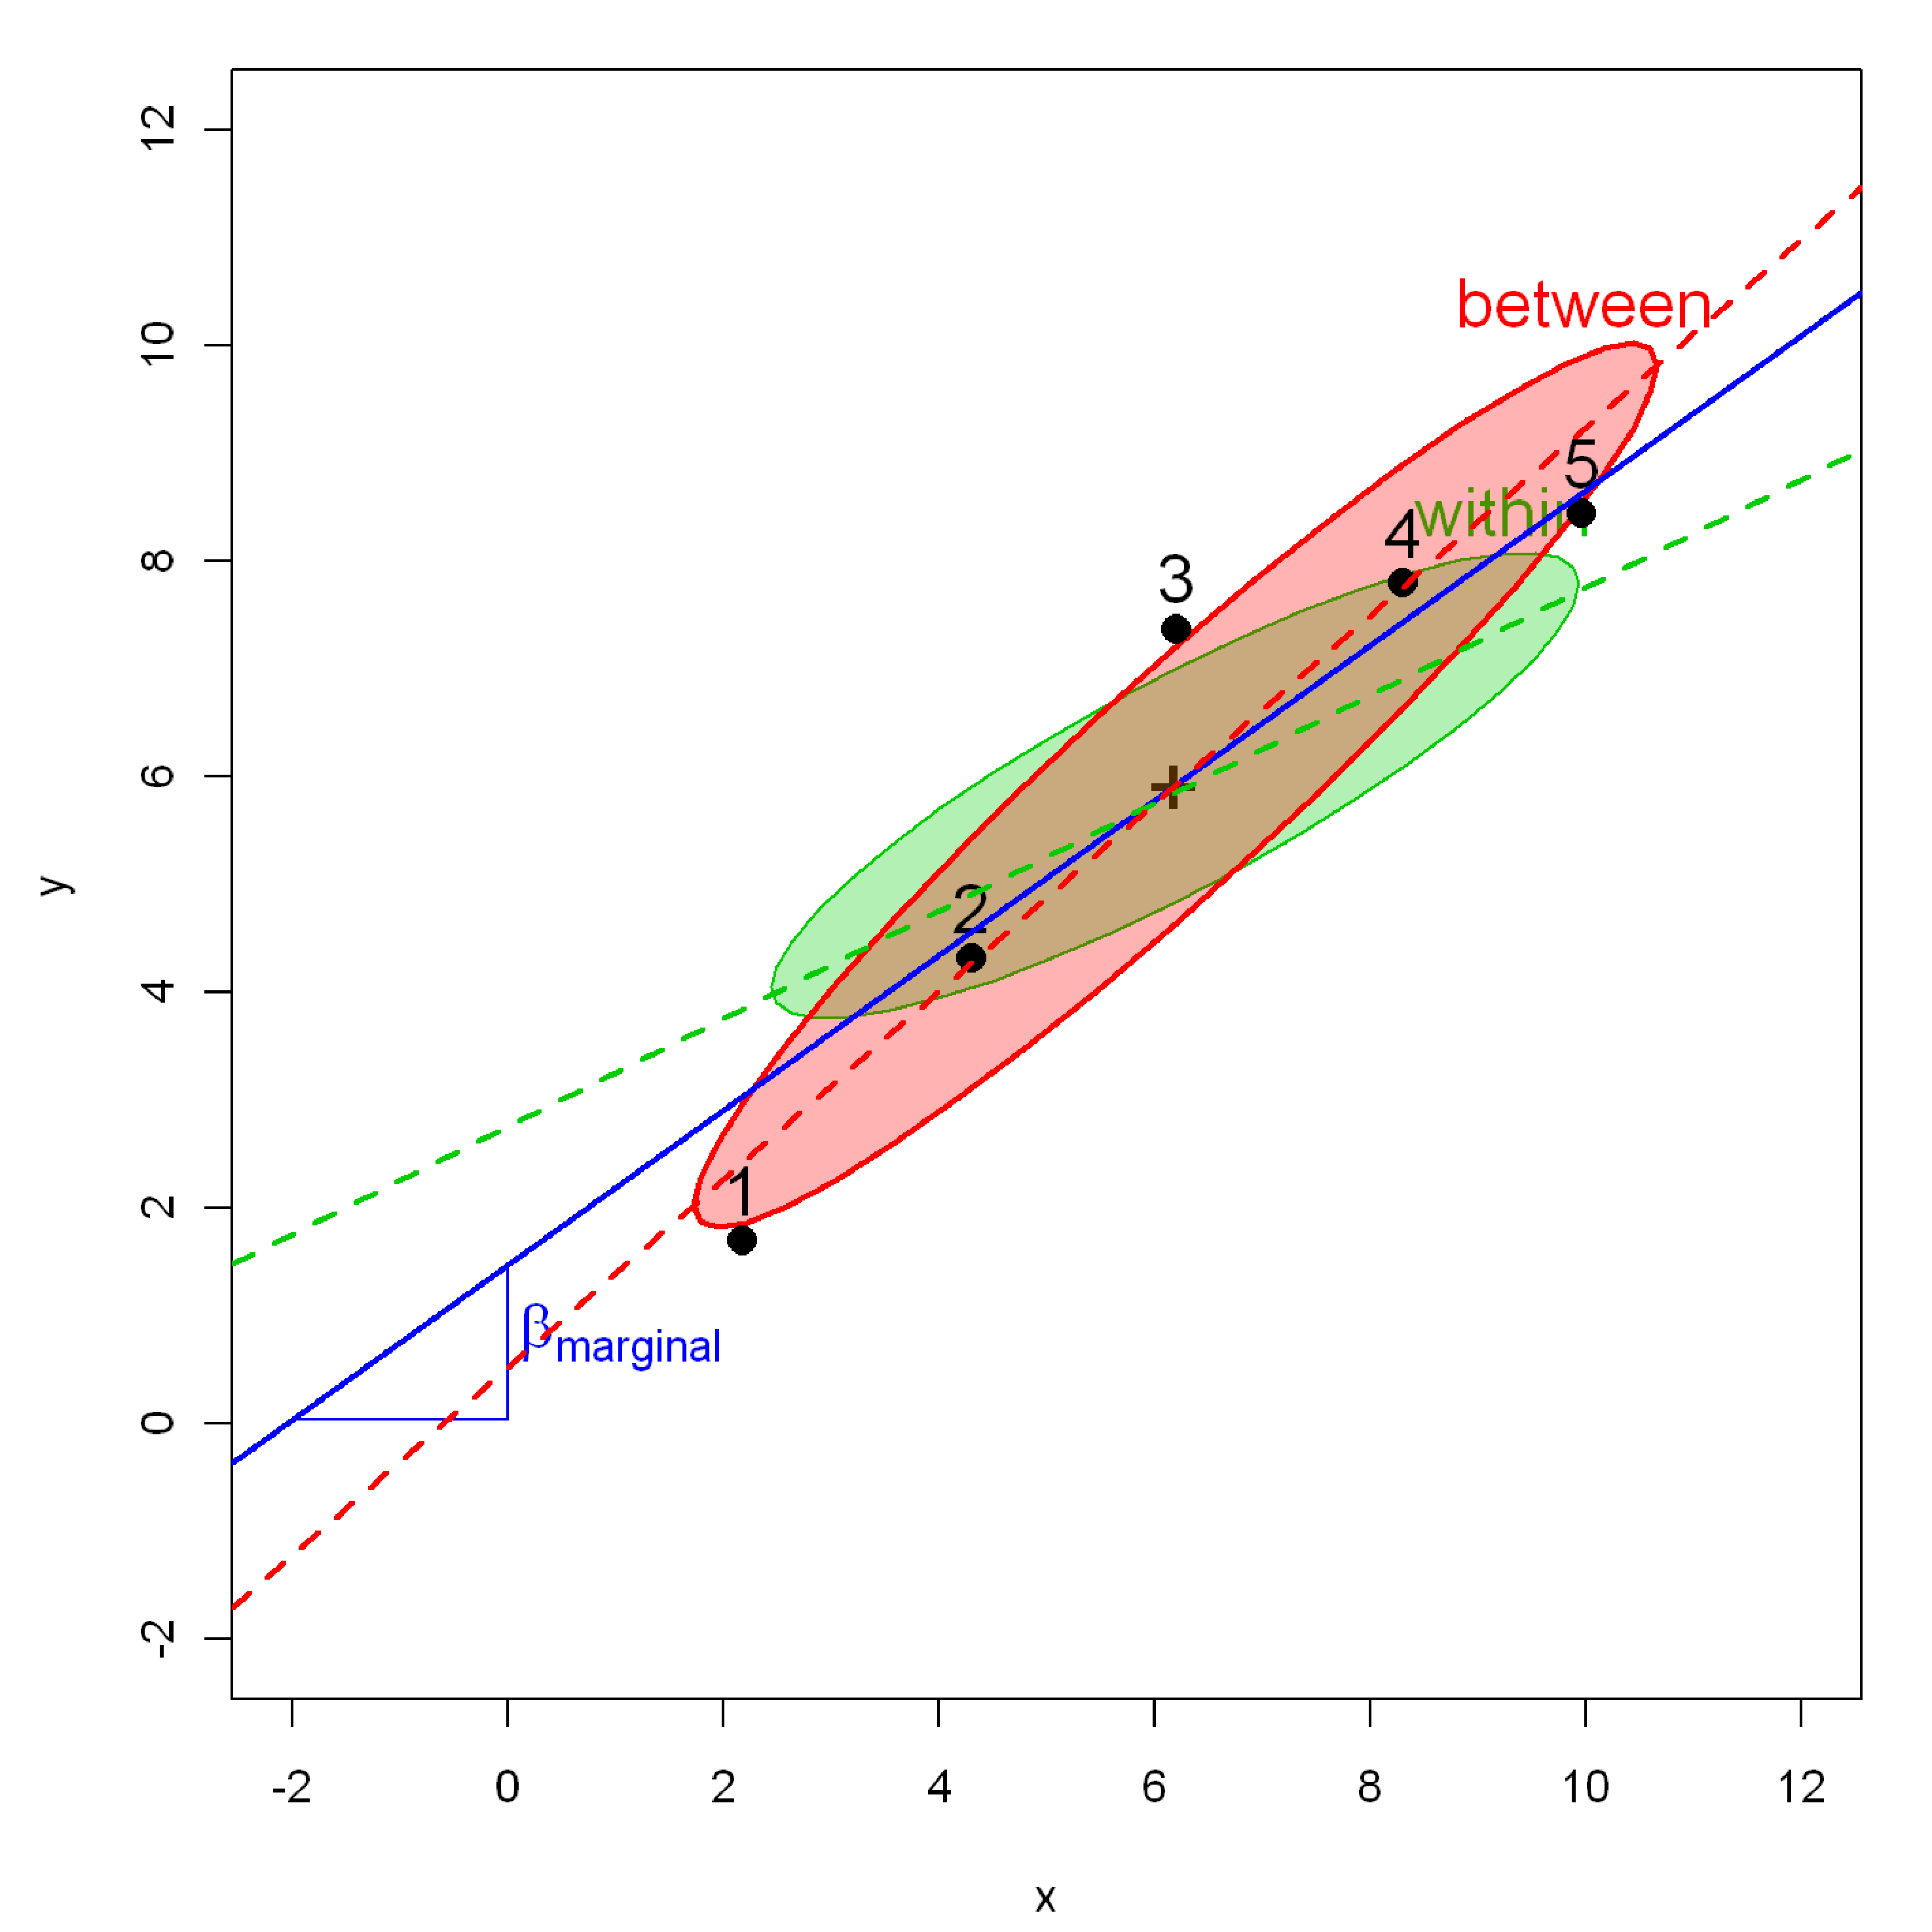
\includegraphics[width=1\linewidth]{fig/between-HE1}
 \end{minipage}%
 \hfill
 \begin{minipage}[b]{.49\linewidth}
  \centering
  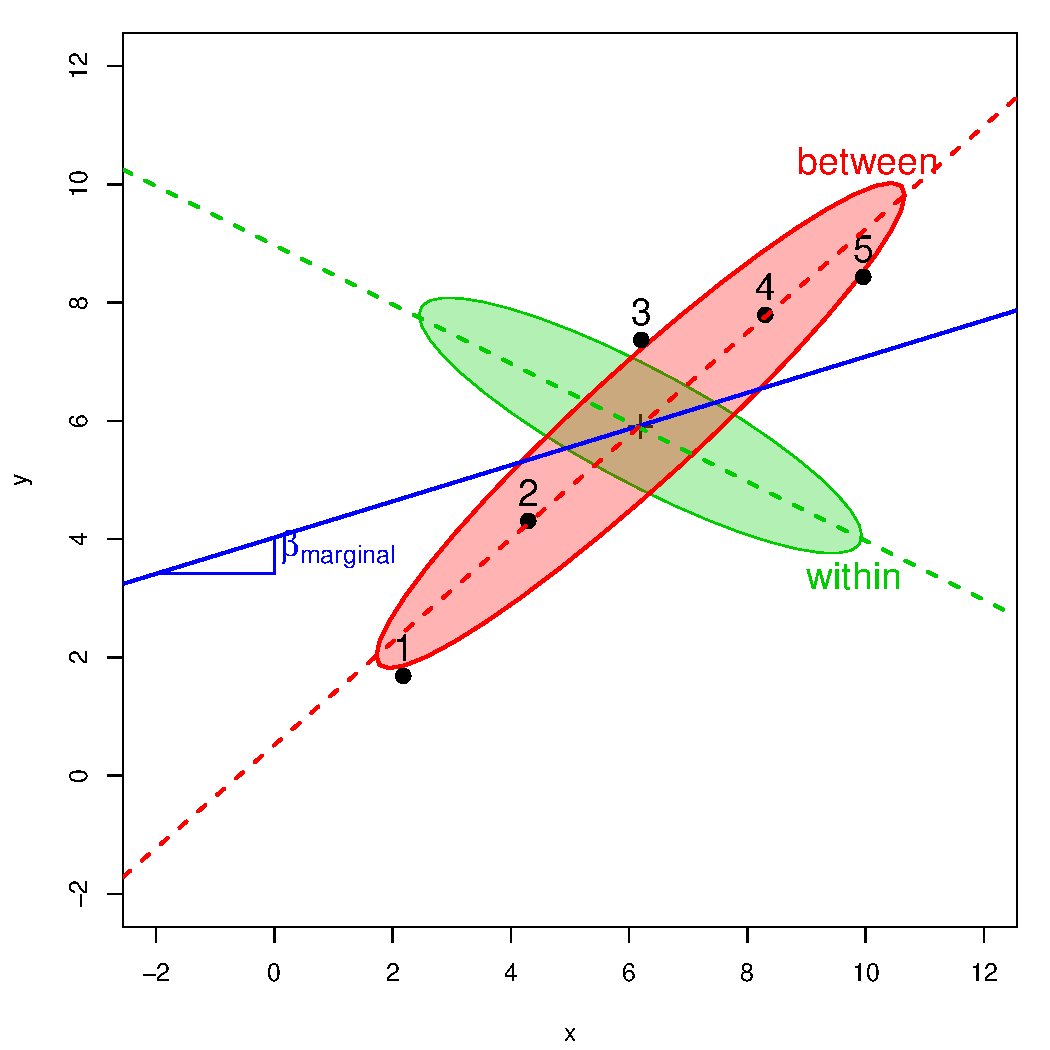
\includegraphics[width=1\linewidth]{fig/between-HE2}
 \end{minipage}
  \caption{Visual demonstration that $\vec{\beta}_{\textrm{marginal}}$ lies between $\vec{\beta}_{\textrm{within}}$ and $\vec{\beta}_{\textrm{between}}$.
  Each panel shows an HE plot for the MANOVA model $(x, y) \sim \textrm{group}$, in which the within and between ellipses are identical to
  those in \figref{fig:between-within}, except for scale.}
  \label{fig:between-HE}
\end{figure}

The right panel of \figref{fig:between-within} provides a prototypical illustration of Simpson's paradox,
where $\beta_{\textrm{within}}$ and $\beta_{\textrm{marginal}}$ can have opposite signs. Underlying this is a
more general \emph{marginal fallacy} (requiring only substantively different estimates, but not necessarily
different signs),
that can occur when some important factor or covariate is unmeasured
or has been ignored. The fallacy consists of estimating the unconditional or marginal
relationship ($\beta_{\textrm{marginal}}$) and believing that it reflects the conditional relationship, or that
those pesky ``other'' variables will somehow average out. In practice, the marginal fallacy probably occurs most
often when one views a scatterplot matrix of $(y, x_1, x_2, \dots)$ and believes that the slopes of
relationships in the separate panels reflect the pairwise conditional relationships with other variables
controlled. In a regression context, the antidote to the marginal fallacy is the added-variable
plot (described in \secref{sec:avp}),
which displays the conditional relationship between the response and a predictor directly, controlling for all other predictors.

The right panel of \figref{fig:between-within} also illustrates Robinson's paradox \citep{Robinson:1950},
where $\beta_{\textrm{within}}$ and $\beta_{\textrm{between}}$ can have opposite signs.%
\footnote{
William Robinson \citeyearpar{Robinson:1950} examined the relationship between literacy rate and percentage
of foreign-born immigrants in the U.S. states from the 1930 Census.
He showed that there was a surprising
positive correlation, $r_{\textrm{between}}= 0.526$ at the state level,
suggesting that foreign birth was associated with greater literacy;
at the individual level, the correlation $r_{\textrm{within}}$ was $-0.118$, suggesting the opposite.
An explanation for the paradox was that immigrants tended to settle in regions of greater than
average literacy.
}
The more general \emph{ecological fallacy} (e.g., \citealp{Freedman:01})
is to draw conclusions from aggregated data, estimating
$\beta_{\textrm{between}}$ or $r_{\textrm{between}}$, believing that they reflect relationships
at the individual level, estimating $\beta_{\textrm{within}}$ or $r_{\textrm{within}}$.
Perhaps the earliest instance of this was Andr\'e-Michel Guerry's \citeyearpar{Guerry:1833} use of thematic maps of
France depicting rates of literacy, crime, suicide, and other ``moral statistics'' by department to argue
about the relationships of these moral variables as if they reflected individual behavior.%
\footnote{
Guerry was certainly aware of the logical problem of ecological inference, at least in general terms
\citep{Friendly:07:guerry}, and carried out several side-analyses to examine potential confounding
variables.
}
As can be seen in \figref{fig:between-within}, the ecological fallacy can often be resolved
by accounting for some confounding variable(s) that vary between groups.

Finally, there are situations where only a subset of the relevant data are available (e.g.,
one group in \figref{fig:between-within}), or when the relevant data are available only
at the individual level,
so that only the conditional relationship,
$\beta_{\textrm{within}}$ can be estimated. The \emph{atomistic fallacy}
(sometimes called the \emph{fallacy of composition})
is the inverse to the
ecological fallacy, and consists of believing that one can draw conclusions
about the ecological relationship, $\beta_{\textrm{between}}$, from the conditional one.

The atomistic fallacy occurs most often in the context of multilevel models,
where it is desired to draw inferences regarding variability of higher-level units
(states, countries) from data collected from lower-level units.
For example, imagine that the right panel of \figref{fig:between-within} depicts the negative
relationship of mortality from heart disease ($y$) with individual income ($x$) for
individuals within countries. It would be fallacious to infer that the same slope
(or even its sign) applies to a between-country analysis of heart disease mortality vs.
GNP per capita. A positive value of $\beta_{\textrm{between}}$ in this context might
result from the fact that, across countries, higher GNP per capita is associated with
less healthy diet (more fast food, red meat, larger portions), leading to increased heart disease.


\subsection{Leverage, influence, \emph{and} precision}

\begin{figure}[htb!]
  \centering
  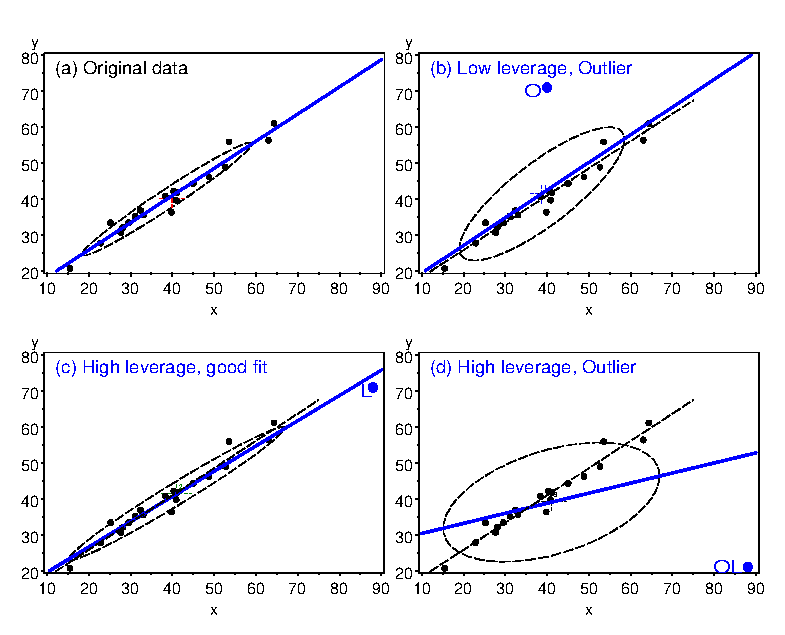
\includegraphics[width=.9\textwidth,clip]{fig/levdemo21}
  \caption{Leverage-Influence quartet with data ellipses. (a) Original data;
  (b) adding one low-leverage outlier (O); (c) adding one ``good'' leverage point (L);
  (d) adding one ``bad'' leverage point (OL).
  In panels (b)--(d) the dashed black line is the fitted line for the original
  data, while the thick solid blue line reflects the  regression including the additional point.
  The data ellipses show the effect of the additional point on precision.}%
  \label{fig:levdemo21}
\end{figure}

The topic of leverage and influence in regression is often introduced with graphs
similar to \figref{fig:levdemo21}, what we call
the ``leverage-influence quartet.''
In these graphs, a bivariate sample of $n=20$ points was first generated
with $x \sim \mathcal{N}(40, 10^2)$ and $y \sim 10 +  0.75 x + \mathcal{N}(0, 2.5^2)$.
Then, in each of
panels (b)--(d) a single point was added at the locations shown, to represent, respectively,
a low-leverage point with a large residual,%
\footnote{In this context, a residual is ``large'' when the point in question deviates substantially from the
regression line for the rest of the data---what is sometimes termed a ``deleted residual''; see below.} 
a high-leverage point with small residual
(a ``good'' leverage point), and a high-leverage point with large residual
(a ``bad'' leverage point).  The goal is to visualize how leverage [$\propto (x-\bar{x})^2$] and
residual ($y - \hat{y}^{*}$) (where $\hat{y}^{*}_{i}$ is the fitted value for observation $i$, computed on the basis of an auxiliary regression in which observation $i$ is deleted) combine to produce influential points---those that affect
the estimates of $\vec{\beta} = (\beta_0 , \beta_1)\trans$.


The ``standard'' version of this graph shows \emph{only} the fitted regression lines for each
panel. So, for the moment, ignore the data ellipses in the plots.
The canonical, first-moment-only, story behind the standard version is that the points added in panels
(b) and (c) are not harmful---the fitted line does not change very much when these
additional points are included. Only the bad leverage point, ``OL,'' in panel (d) is harmful.

\begin{figure}[htb!]
  \centering
  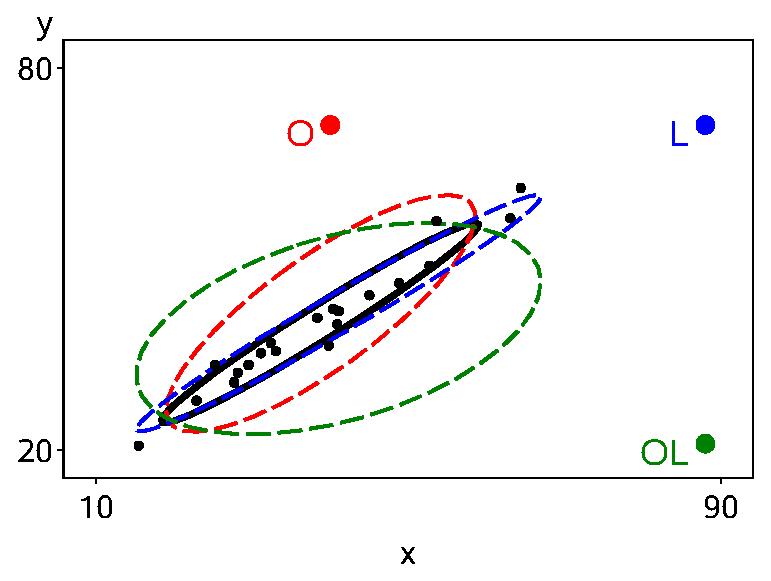
\includegraphics[width=.5\textwidth,clip]{fig/levdemo22}
  \caption{Data ellipses in the Leverage-Influence quartet. This graph overlays the data ellipses
  and additional points from the four panels of \figref{fig:levdemo21}. It can be seen that only the
  OL point affects the slope, while the O and L points affect precision of the estimates in opposite
  directions.}%
  \label{fig:levdemo22}
\end{figure}

Adding the data ellipses to each panel immediately makes it clear that there is a second-moment
part to the the story---the effect of unusual points on the \emph{precision} of our estimates
of $\vec{\beta}$.  Now,
we see \emph{directly} that there is a big difference in impact between
the low-leverage outlier [panel (b)] and the high-leverage, small-residual case [panel (c)],
even though their effect on coefficient estimates is negligible.
In panel (b), the single outlier inflates the estimate of residual variance (the size of the
vertical slice of the data ellipse at $\bar{x}$).

To make the added value of the data ellipse more apparent, we overlay the data ellipses from
\figref{fig:levdemo21} in a single graph, shown in
\figref{fig:levdemo22}, to allow direct comparison.  Because you now know that regression lines
can be visually estimated as the locus of vertical tangents, we suppress these lines in the
plot to focus on precision.  Here, we can also see why the high-leverage
point ``L'' [added in panel (c) of \figref{fig:levdemo21}] is called a ``good leverage point.''
By increasing the standard deviation of $x$, it makes the data ellipse somewhat more elongated,
giving increased precision of our estimates of $\vec{\beta}$. 

Whether a ``good'' leverage point is \emph{really} good depends upon our faith in the regression model (and in the point), 
and may be regarded either as increasing the precision of $\hat{\vec{\beta}}$ or providing an illusion of precision.
In either case, the data ellipse for the modified data shows the effect on precision directly.


\subsection[Ellipsoids in data space and beta space]{Ellipsoids in data space and $\vec{\beta}$ space}

It is most common to look at data and fitted models in ``data space,'' where axes correspond to
variables, points represent observations, and fitted models are plotted as lines (or planes) in this space.
As we've suggested, data ellipsoids provide informative summaries of relationships in data space.
For linear models, particularly regression models with quantitative predictors, there is another space---$\vec{\beta}$ space---that provides deeper views of models and the relationships among them.
In $\vec{\beta}$ space, the axes pertain to coefficients and points are models (true, hypothesized, fitted) whose coordinates
represent values of parameters.

In the sense described below, data space and $\vec{\beta}$ space are \emph{dual} to each other.
In simple linear regression, for example, each line in data space corresponds to a point in $\vec{\beta}$ space,
the set of points on any line in $\vec{\beta}$ space corresponds to a pencil of lines through a given point
in data space, and the proposition that every pair of points defines a line in one space corresponds to
the proposition that every two lines intersect in a point in the other space.

Moreover, ellipsoids in these spaces are dual and inversely related to each other.
In data space, joint confidence intervals for the mean vector or joint prediction
regions for the data are given by the ellipsoids $\bar{y} \oplus c \sqrt{\mat{S}}$.
In the dual $\vec{\beta}$ space, joint confidence regions for the parameters
are given by ellipsoids of the form $\hat{\beta} \oplus c \sqrt{\mat{S}^{-1}}$.
We illustrate these relationships in the example below.

\begin{figure}[htb]
  \centering
  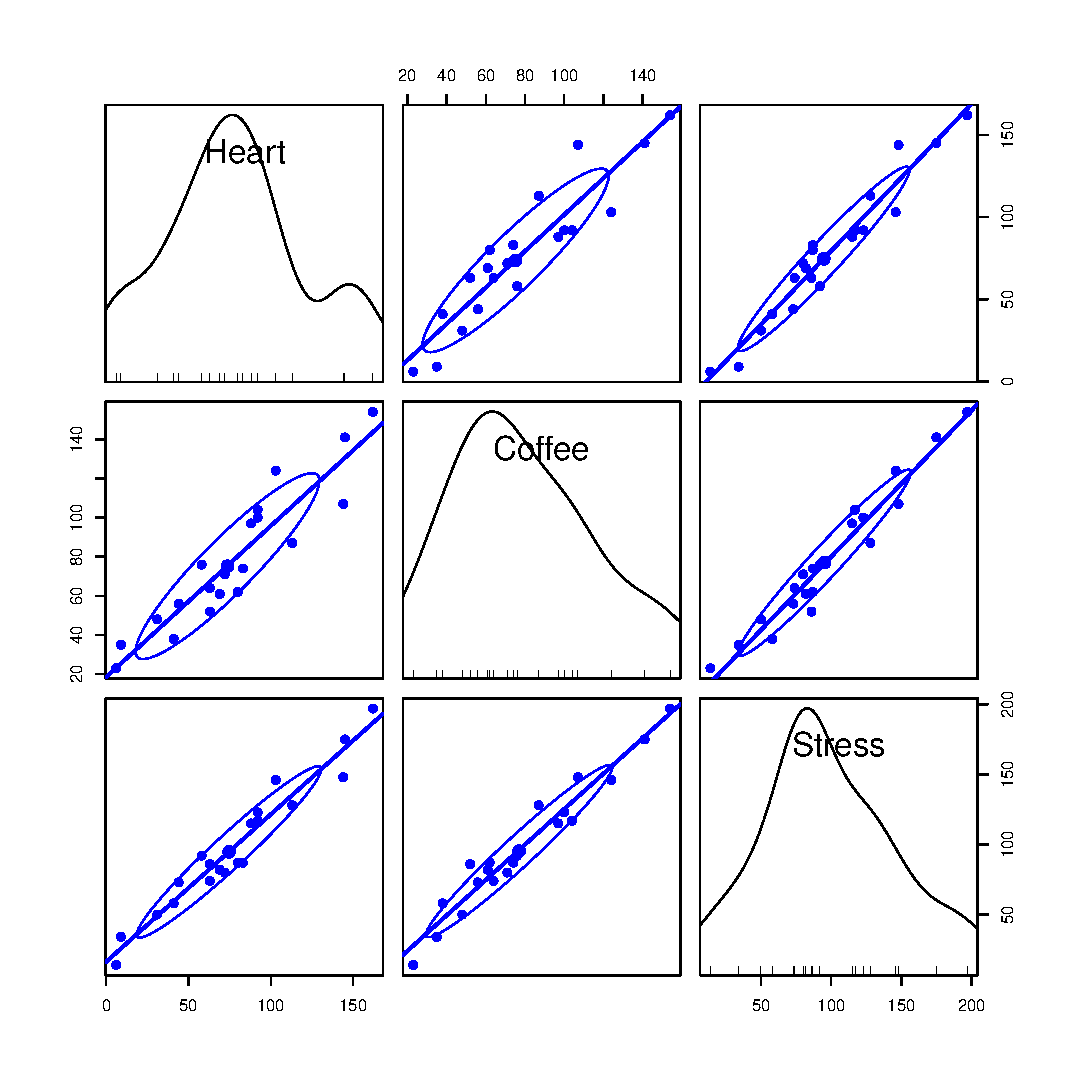
\includegraphics[width=.6\textwidth,clip]{fig/vis-reg-coffee11}
  \caption{Scatterplot matrix, showing the pairwise relationships among Heart ($y$), Coffee ($x_1$), and Stress ($x_2$),
  with linear regression lines and 68\% data ellipses for the marginal bivariate relationships.
  }%
  \label{fig:vis-reg-coffee11}
\end{figure}

\figref{fig:vis-reg-coffee11} shows a scatterplot matrix among the variables
Heart ($y$), an index of cardiac damage; Coffee ($x_1$), a measure of daily
coffee consumption; and Stress ($x_2$), a measure of occupational stress, in a contrived
sample of $n=20$. For the sake of the example we assume that the main goal is
to determine whether or not coffee is good or bad for your heart, and stress
represents one potential confounding variable among others (age, smoking, etc.)
that might be useful to control statistically.

The plot in \figref{fig:vis-reg-coffee11} shows only the marginal relationship
between each pair of variables. The marginal message seems to be that coffee is
bad for your heart, stress is bad for your heart and coffee consumption is
also related to occupational stress.
\begin{figure}[htb]
% two figs side-by-side
  \begin{minipage}[c]{.485\textwidth}
   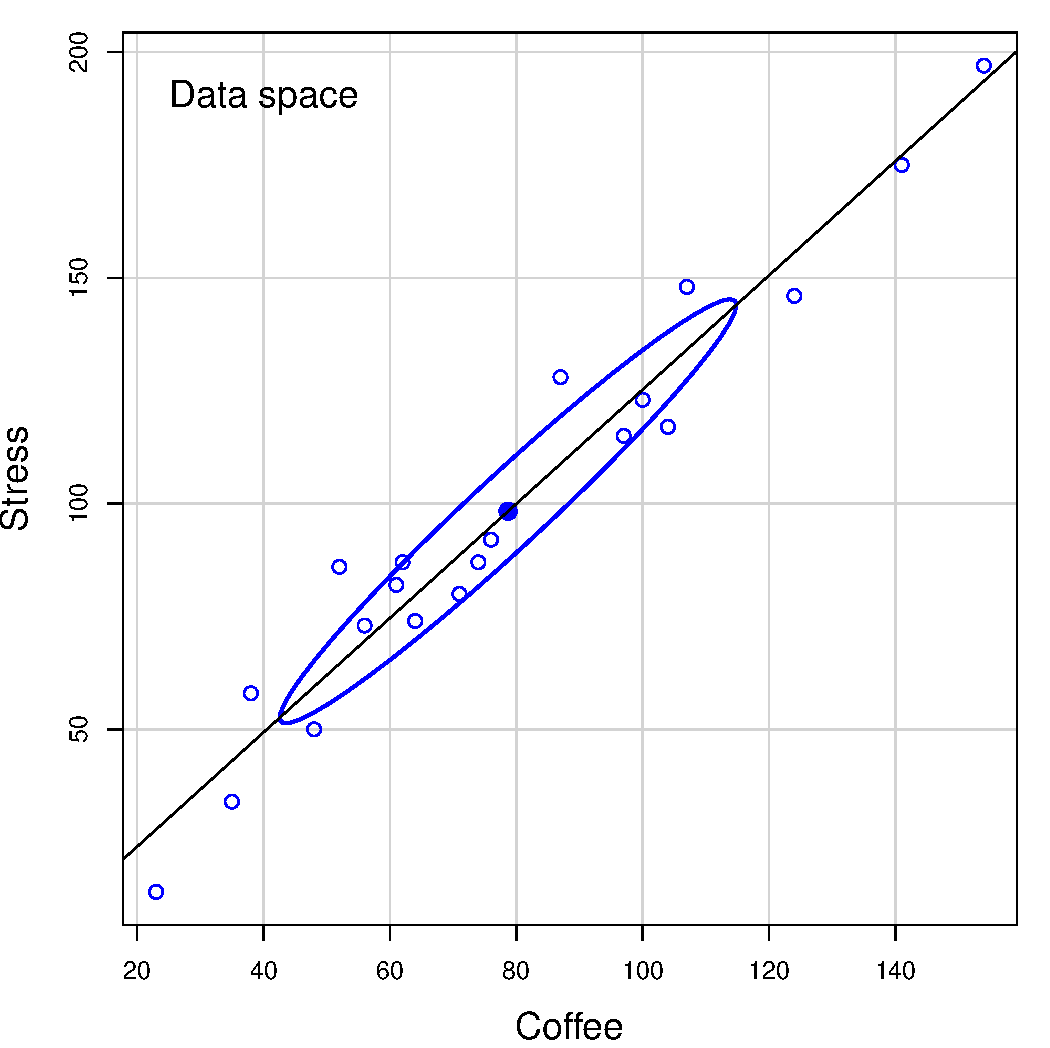
\includegraphics[width=1\linewidth,clip]{fig/vis-reg-coffee12a}
   \end{minipage}%
  \hfill
  \begin{minipage}[c]{.485\textwidth}
   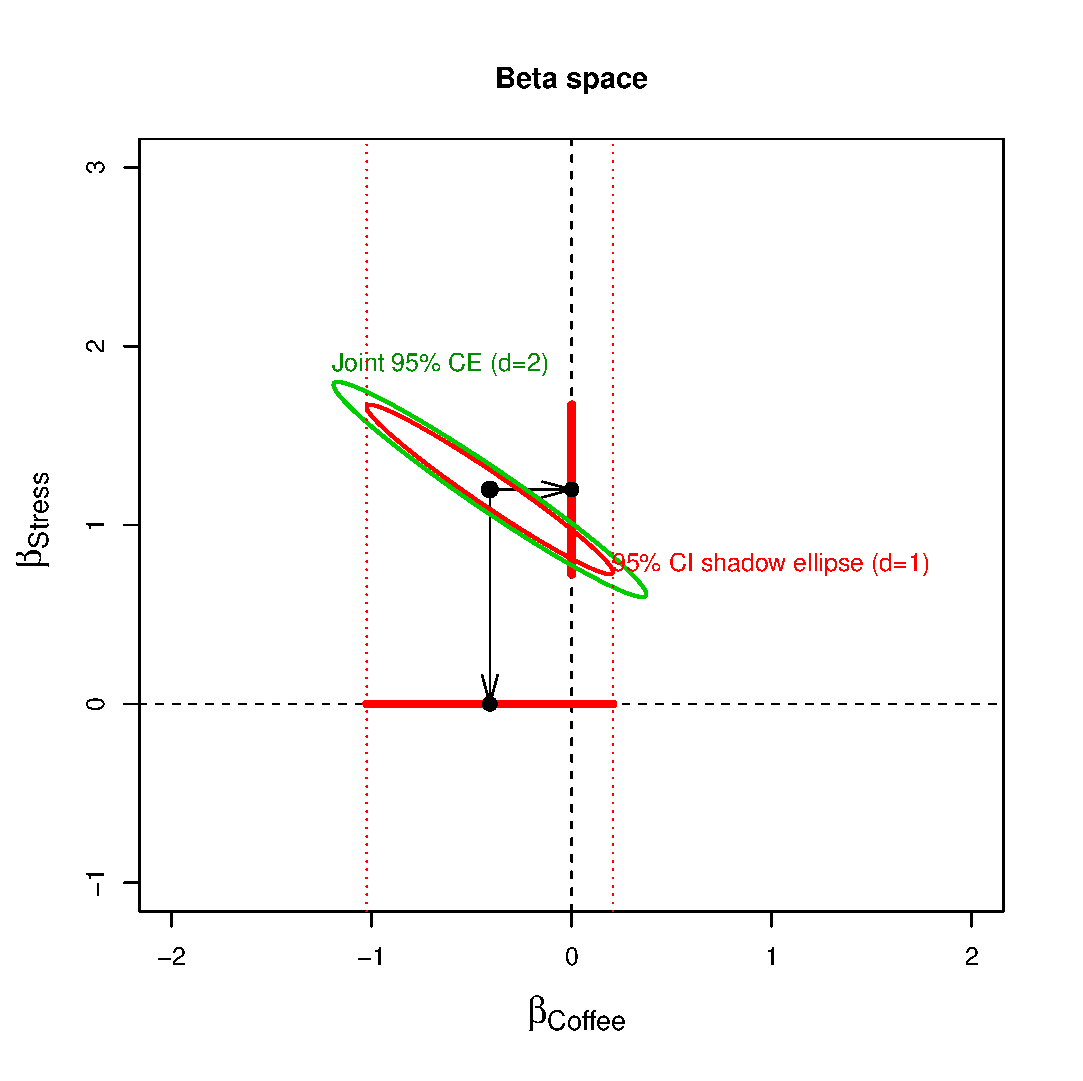
\includegraphics[width=1\linewidth,clip]{fig/vis-reg-coffee12b}
  \end{minipage}
  \caption{Data space and $\vec{\beta}$ space representations of Coffee and Stress.
   Left: Standard (40\%) data ellipse. Right: Joint 95\% confidence ellipse (green) for
   ($\beta_{\mathrm{Coffee}}, \beta_{\mathrm{Stress}}$), CI ellipse (red) with 95\% univariate shadows.
  }%
  \label{fig:vis-reg-coffee12}
\end{figure}
Yet, when we fit both variables together, we obtain the following results,
suggesting that coffee is good for you (the coefficient for coffee is now
negative, though non-significant).  How can this be?

% latex table generated in R 2.12.2 by xtable 1.5-6 package
% Fri Jun 03 09:01:43 2011
%\begin{table}[ht]
\begin{center}
\begin{tabular}{lrrrr}
%  \hline
 & Estimate ($\widehat{\beta}$) & Std. Error & $t$ value & Pr($>|t|$) \\ 
  \hline
(Intercept) & -7.7943 & 5.7927 & -1.35 & 0.1961 \\ 
  Coffee & -0.4091 & 0.2918 & -1.40 & 0.1789 \\ 
  Stress & 1.1993 & 0.2244 & 5.34 & 0.0001 \\ 
   \hline
\end{tabular}
\end{center}
%\end{table}

%\begin{verbatim}
%Coefficients:
%            Estimate Std. Error t value Pr(>|t|)
%(Intercept)  -7.7943     5.7927  -1.346    0.196
%Coffee       -0.4091     0.2918  -1.402    0.179
%Stress        1.1993     0.2244   5.345 5.36e-05 ***
%---
%Signif. codes:  0 '***' 0.001 '**' 0.01 '*' 0.05 '.' 0.1 ' ' 1
%
%Residual standard error: 10.36 on 17 degrees of freedom
%Multiple R-squared: 0.9462,     Adjusted R-squared: 0.9399
%F-statistic: 149.6 on 2 and 17 DF,  p-value: 1.620e-11
%\end{verbatim}

\figref{fig:vis-reg-coffee12} shows the relationship between the
predictors in data space and how this translates into joint and
individual confidence intervals for the coefficients in
$\vec{\beta}$ space.  The left panel is the same as the corresponding
(Coffee, Stress) panel in \figref{fig:vis-reg-coffee11}, but with
a standard (40\%) data ellipse. The right panel shows the joint 95\% confidence
region and the individual 95\% confidence intervals in $\vec{\beta}$ space, determined as
\begin{equation*}
 \widehat{\beta} \oplus \sqrt{d F^{.95}_{q, \nu}} \times s_e \times \mat{S}_X^{-1/2}
\end{equation*}
where $d$ is the number of dimensions for which we want coverage,
$\nu$ is the residual degrees of freedom for $s_e$, and $\mat{S}_X$
is the covariance matrix of the predictors.

Thus, the green ellipse in \figref{fig:vis-reg-coffee12} is the
ellipse of joint 95\% coverage, using the factor $\sqrt{2 F^{.95}_{2, \nu}}$
and covering the true values of ($\beta_{\mathrm{Stress}}, \beta_{\mathrm{Coffee}}$)
in 95\% of samples.  Moreover:
\begin{itemize*}
  \item Any \emph{joint} hypothesis (e.g., $H_0:\beta_{\mathrm{Stress}}=1, \beta_{\mathrm{Coffee}}=1$)
can be tested visually, simply by observing whether the
hypothesized point, $(1, 1)$ here, lies inside or outside the joint ellipse.
  \item The shadows of this ellipse on the horizontal and vertical axes
give Scheff\'e joint 95\%  confidence intervals for each parameter, with protection for ``fishing''
in a 2-dimensional space.
  \item Similarly, using the factor
$\sqrt{F^{1-\alpha/d}_{1, \nu}} = t^{1-\alpha/2d}_\nu$ would give an
ellipse whose 1D shadows are $1-\alpha$ Bonferroni confidence intervals
for $d$ posterior hypotheses.
\end{itemize*}

Visual hypothesis tests and $d=1$ confidence intervals for the parameters \emph{separately}
are obtained from the red ellipse in \figref{fig:vis-reg-coffee12},
which is scaled by $\sqrt{F^{.95}_{1, \nu}} = t^{.975}_\nu$. We call this the ``confidence-interval generating ellipse'' (or, more compactly, the ``confidence-interval ellipse'').
The shadows of the confidence-interval ellipse on the axes (thick red lines) give the
corresponding individual 95\% confidence intervals, which are
equivalent to the (partial, Type III) $t$-tests for each coefficient given in the
standard multiple regression output shown above.
Thus, controlling for Stress, the confidence interval for the slope for Coffee includes 0,
so we cannot reject the hypothesis that $\beta_{\mathrm{Coffee}}=0$
in the multiple regression model, as we saw above in the numerical output.
On the other hand, the interval for the slope for Stress excludes the origin,
so we reject the null hypothesis that $\beta_{\mathrm{Stress}}=0$,
controlling for Coffee consumption.

Finally, consider the relationship between the data ellipse and the
confidence ellipse.  These have exactly the same shape, but
(with equal coordinate scaling of the axes), the confidence ellipse
is exactly a $90^o$ rotation of the data ellipse.  In directions in
data space where the data ellipse is wide---where we have more information
about the relationship between Coffee and Stress---the confidence ellipse is
narrow, reflecting greater precision of the estimates of coefficients.
Conversely, where the data ellipse is narrow (less information), the
confidence ellipse is wide (less precision).

\begin{figure}[htb]
  \centering
  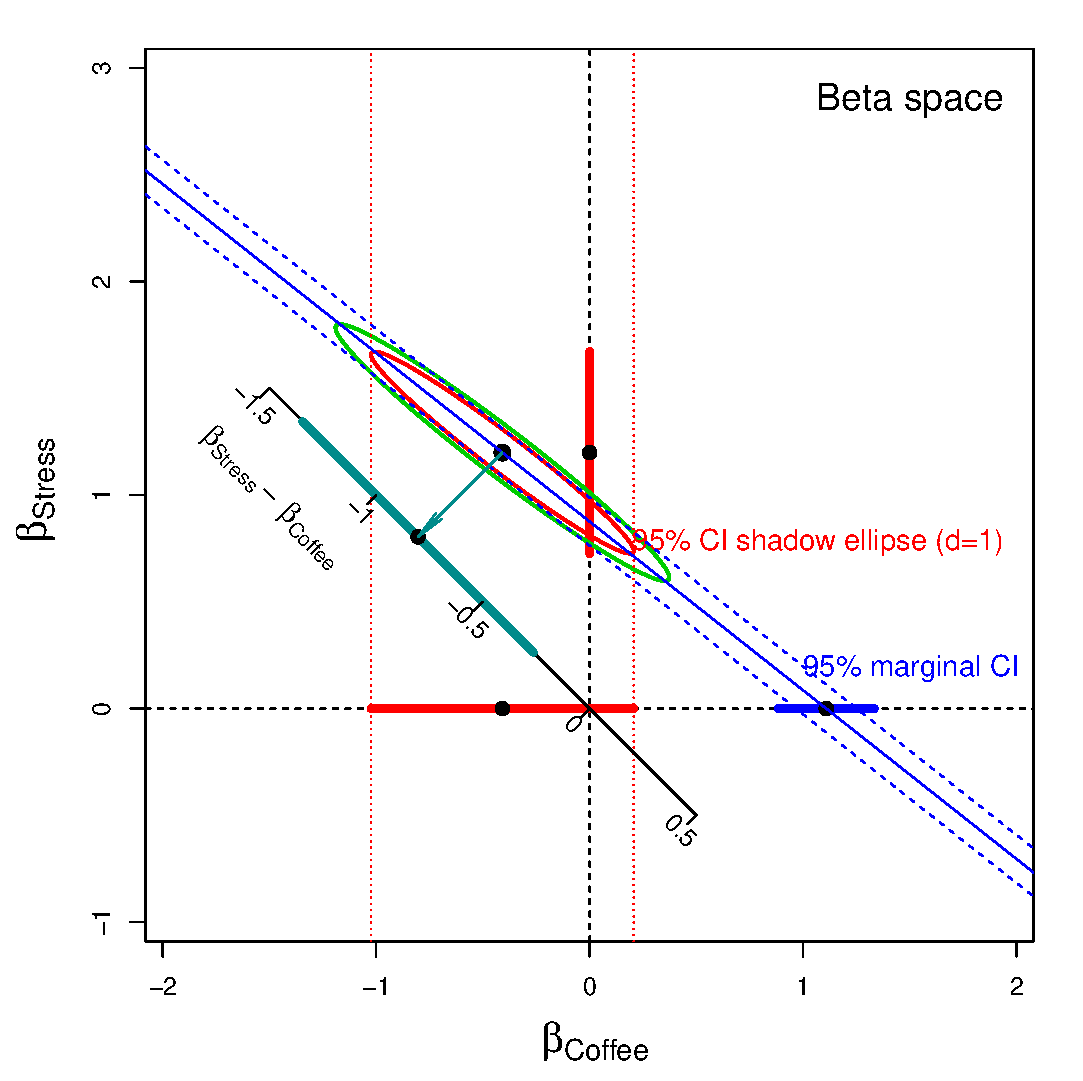
\includegraphics[width=.6\textwidth,clip]{fig/vis-reg-coffee13}
  \caption{Joint 95\% confidence ellipse for ($\beta_{\mathrm{Coffee}}, \beta_{\mathrm{Stress}}$),
  together with the 1D marginal confidence interval for $\beta_{\mathrm{Coffee}}$
  ignoring Stress (thick blue line), and a visual confidence interval for $\beta_{\mathrm{Stress}} - \beta_{\mathrm{Coffee}}=0$
  (dark cyan).
  }%
  \label{fig:vis-reg-coffee13}
\end{figure}

The virtues of the confidence ellipse for visualizing hypothesis tests and interval estimates
do not end here. Say we wanted to test the hypothesis that Coffee was unrelated to Heart damage
in the \emph{simple} regression ignoring Stress.  The (Heart, Coffee) panel in \figref{fig:vis-reg-coffee11}
showed the strong marginal relationship between the variables.  This can be seen in \figref{fig:vis-reg-coffee13} as
the oblique projection of the confidence ellipse to the horizontal axis where $\beta_{\mathrm{Stress}}=0$.
The estimated slope for Coffee in the simple regression is exactly the oblique shadow of
the center of the ellipse $(\widehat{\beta}_{\mathrm{Coffee}}, \widehat{\beta}_{\mathrm{Stress}})$
through the point where the ellipse has a horizontal tangent onto the horizontal axis at
$\beta_{\mathrm{Stress}}=0$. The thick blue line in this figure shows the confidence interval
for the slope for Coffee in the simple regression model. The confidence interval doesn't cover the origin, so
we reject $H_0: \beta_{\mathrm{Coffee}} = 0$ in the simple regression model.
The oblique shadow of the red 95\% confidence-interval ellipse onto the horizontal axis
is slightly smaller.  How much smaller is a function of the size of the coefficient for Stress.

%\begin{ADDED} %: 10-21-2011 MF
%\figref{fig:vis-reg-coffee13} has another visual interpretation in the context of \emph{mediation} models
%\citep{MacKinnon:2008}, where we are primarily interested in testing a direct, possibly causal relationship,
%$X \rightarrow Y$, but want to determine if that relation can be explained by an indirect relationship,
%$X \rightarrow M \rightarrow Y$ through a mediating $M$ variable that is correlated with both $X$ and $Y$.
%In this context, $X$ is Coffee, $Y$ is Heart damage and $M$ is Stress.
%In the figure, the significant marginal effect of Coffee ...
%\end{ADDED}

We can go further.  As we noted earlier, all linear combinations of variables or parameters
in data or models correspond graphically to projections (shadows) onto certain sub-spaces.
Let's assume that Coffee and Stress were measured on the same scales\, so it makes sense
to ask if they have equal impacts on Heart disease in the joint model that includes them both.
\figref{fig:vis-reg-coffee13} also shows an auxiliary axis through the origin with slope $=-1$
corresponding to values of $\beta_{\mathrm{Stress}} - \beta_{\mathrm{Coffee}}$. The orthogonal
projection of the coefficient vector on this axis is the point estimate of
$\widehat{\beta}_{\mathrm{Stress}} - \widehat{\beta}_{\mathrm{Coffee}}$
and the shadow of the red ellipse along this axis is the 95\% confidence interval
for the difference in slopes. This interval excludes 0, so we would reject the hypothesis
that Coffee and Stress have equal coefficients.


\subsection{Measurement error}

In classical linear models, the predictors are often considered to be fixed
variables, or, if random, to be measured without error and independent of the regression errors;
either condition, along with the assumption of linearity, guarantees
unbiasedness of the standard OLS estimators.
In practice, of course, predictor variables are often also observed
indicators, subject to error, a fact that is recognized in errors-in-variables
regression models and in more general structural equation models
but often ignored otherwise.  Ellipsoids in data space and $\beta$ space
are well suited to showing the effect of measurement error in predictors on OLS estimates.

\begin{figure}[htb]
 \begin{minipage}[b]{.49\linewidth}
  \centering
  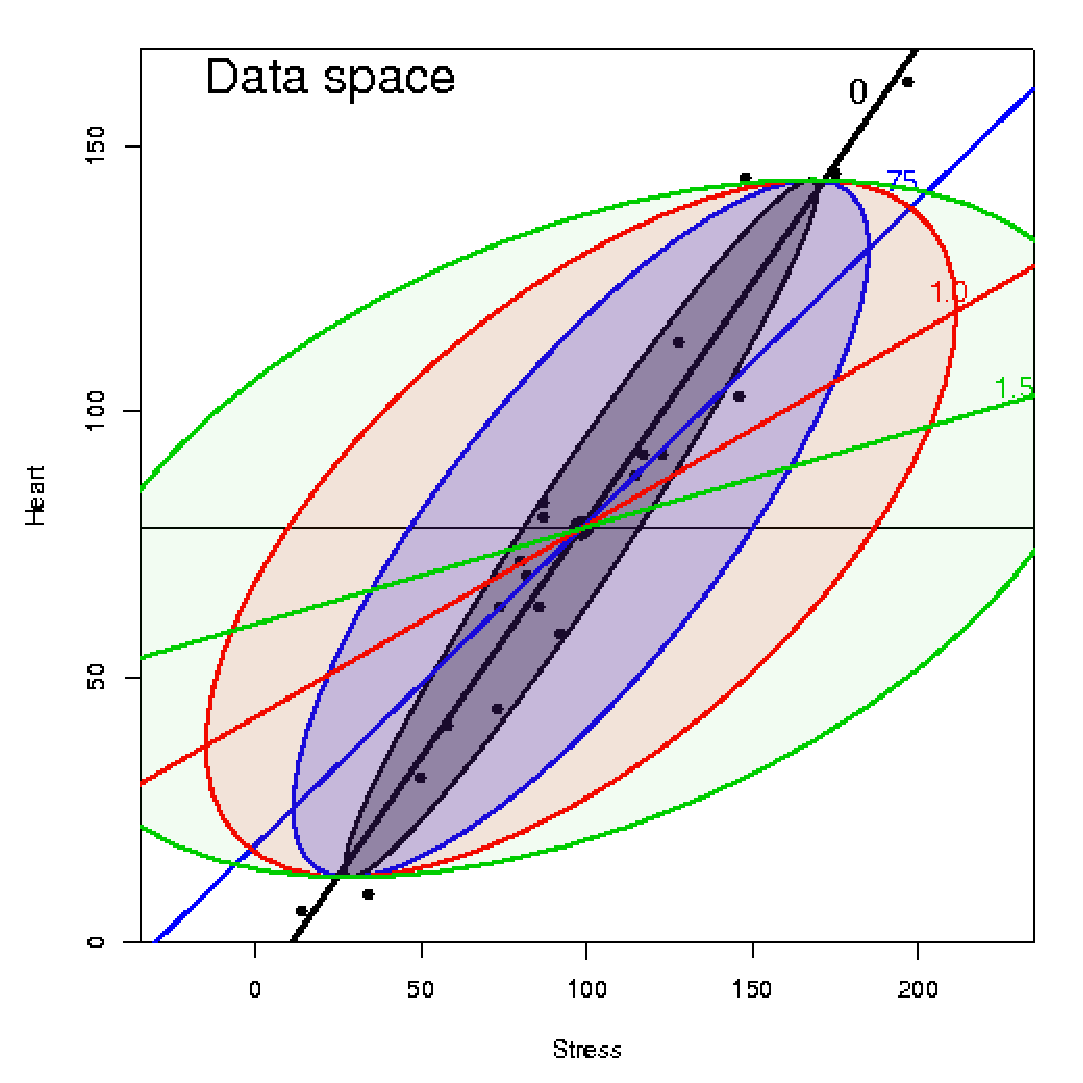
\includegraphics[width=1\linewidth]{fig/coffee-stress1}
%  \caption{}%
%  \label{fig:}
 \end{minipage}%
 \hfill
 \begin{minipage}[b]{.49\linewidth}
  \centering
  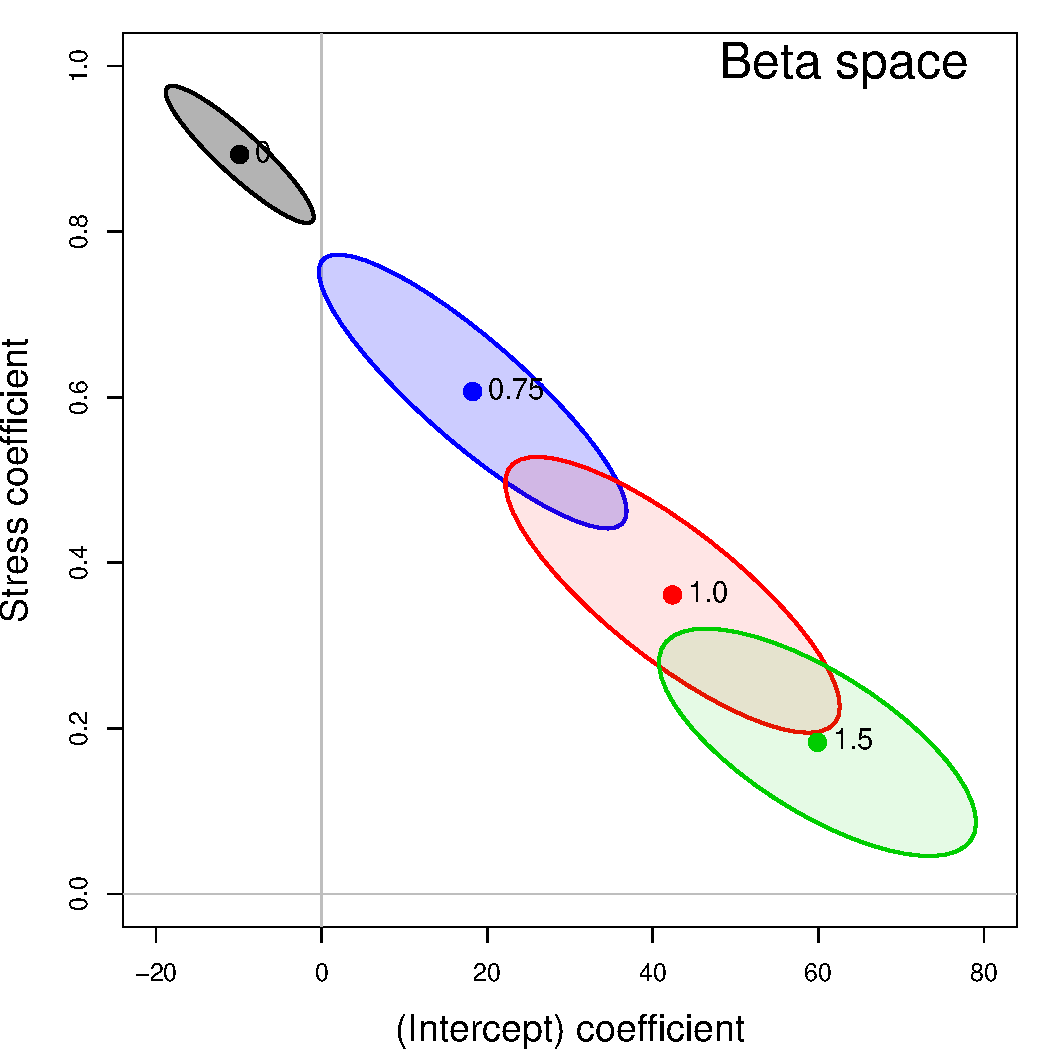
\includegraphics[width=1\linewidth]{fig/coffee-stress2}
 \end{minipage}
  \caption{Effects of measurement error in Stress on the marginal relationship between Heart disease and Stress.
  Each panel starts with the observed data ($\delta=0$), then adds random normal error,
  $\mathcal{N}(0, \delta \times \mathrm{SD}_{Stress})$, with $\delta = \{0.75, 1.0, 1.5\}$, to the value of Stress.
  Increasing measurement error biases the slope for Stress toward 0.
  Left: 50\% data ellipses; right: 50\% confidence ellipses for $(\beta_0, \beta_{Stress})$. }
  \label{fig:coffee-stress}
\end{figure}

The statistical facts are well known, though perhaps counter-intuitive in certain details:
measurement error in a predictor biases regression coefficients, while
error in the measurement in  $y$
increases the standard errors of the regression coefficients but does not introduce
bias.

% DONE
%\TODO{The rest of this section is scheduled for a rewrite (noted by John)}

In the top row of
\figref{fig:vis-reg-coffee11}, adding measurement error to the Heart disease variable
would expand the data ellipses vertically, but 
(apart from random variation)
leaves the slopes of the regression lines unchanged.
Measurement error in a predictor variable, however, biases the corresponding
estimated coefficient toward
zero (sometimes called \emph{regression attenuation}) as well as increasing standard errors.
                                         
\figref{fig:coffee-stress} demonstrates this effect for the marginal
relation between Heart disease and Stress,
with data ellipses in data space and the corresponding confidence ellipses in $\beta$ space.
Each panel starts with the observed data (the darkest ellipse, marked $0$), then adds random normal error,
$\mathcal{N}(0, \delta \times \mathrm{SD}_{Stress})$, with $\delta = \{0.75, 1.0, 1.5\}$, to the value of Stress,
while keeping the mean of Stress the same.
All of the data ellipses have the same vertical shadows ($\mathrm{SD}_{\textrm{Heart}}$), while the horizontal shadows
increase with $\delta$, driving the slope for Stress toward 0.
In $\beta$ space, it can be seen that the estimated coefficients, $(\beta_0, \beta_{\textrm{Stress}})$
vary along a line and approach $\beta_{\textrm{Stress}}=0$ for $\delta$ sufficiently large.
The vertical shadows of
ellipses for $(\beta_0, \beta_{\textrm{Stress}})$ along the $\beta_{\textrm{Stress}}$ axis
also demonstrate the effects of measurement error
on the standard error of $\beta_{\textrm{Stress}}$.

Perhaps less well-known, but both more surprising and interesting, is the effect that measurement error in one variable,
$x_1$, 
has on the estimate of the coefficient for an \emph{other} variable, $x_2$, in a multiple regression model.
\figref{fig:coffee-measerr}
shows the confidence ellipses for $(\beta_{\textrm{Coffee}}, \beta_{\textrm{Stress}})$ in the multiple regression 
predicting Heart disease, adding random normal error
$\mathcal{N}(0, \delta \times \mathrm{SD}_{Stress})$, with $\delta = \{0, 0.2, 0.4, 0.8\}$, to the value of Stress
alone.  
As can be plainly seen, while this measurement error in Stress attenuates its coefficient,
it also has the effect of biasing the coefficient for Coffee toward that in the \emph{marginal}
regression of Heart disease on Coffee alone.


\begin{figure}[htb]
  \centering
  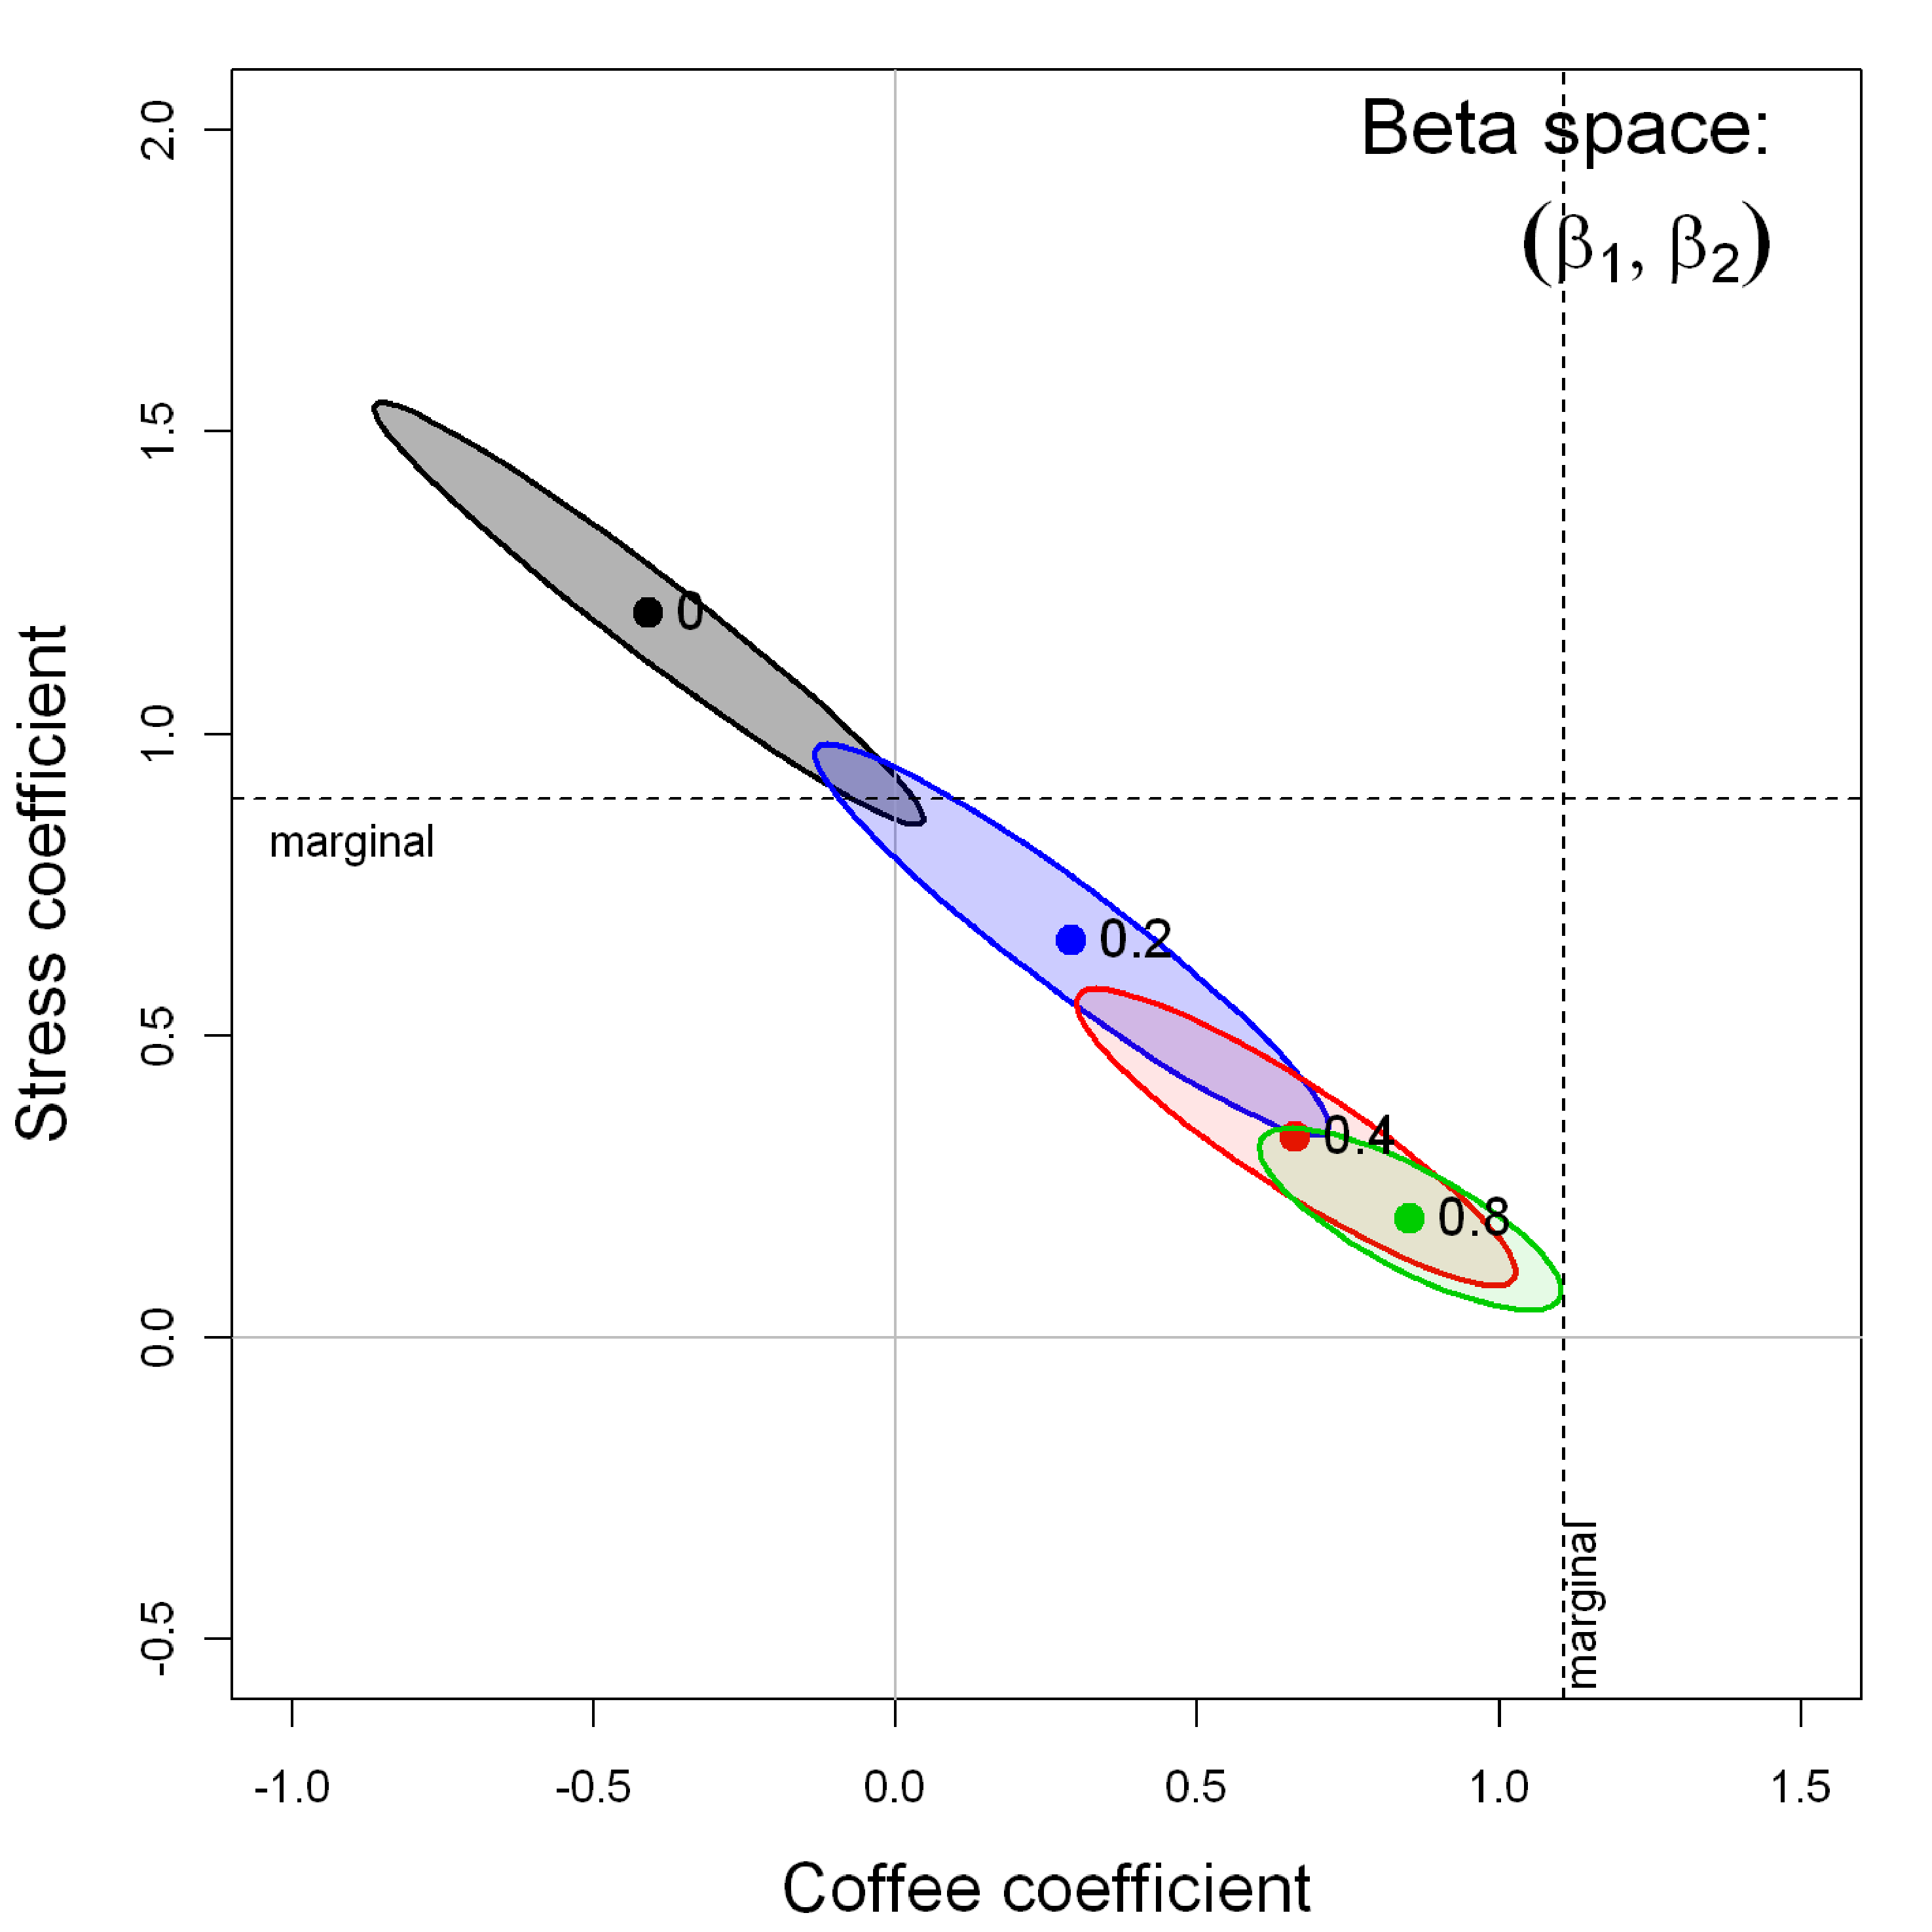
\includegraphics[width=.5\textwidth,clip]{fig/coffee-measerr}
  \caption{Biasing effect of measurement error in one variable (Stress) on on the coefficient of another variable
  (Coffee) in a multiple regression.  The coefficient for Coffee is driven towards its value in the marginal
  model using Coffee alone, as measurement error in Stress makes it less informative in the joint model.
  }%
  \label{fig:coffee-measerr}
\end{figure}

%\TODO{Can we say anything general about the relative decrease in the standard errors of $\beta_{\textrm{Coffee}}$
%with increasing error in Stress?}

%This effect is entirely understandible from a geometric perspective: increasing measurement error in $x_1$
%makes it less informative for the partial coefficient of $x_2$ 


\subsection{Ellipsoids in added-variable plots}\label{sec:avp}

In contrast to the marginal, bivariate views of the relationships of a response to several predictors (e.g., such as shown in the top row of the scatterplot matrix in \figref{fig:vis-reg-coffee11}), \emph{added-variable plots}
(aka \emph{partial regression plots}) show the partial relationship between the response and
each predictor, where the effects of all other predictors have been controlled or adjusted for.
Again we find that such plots have remarkable geometric properties, particularly
when supplemented by ellipsoids.

\begin{figure}[htb]
 \begin{minipage}[b]{.49\linewidth}
  \centering
  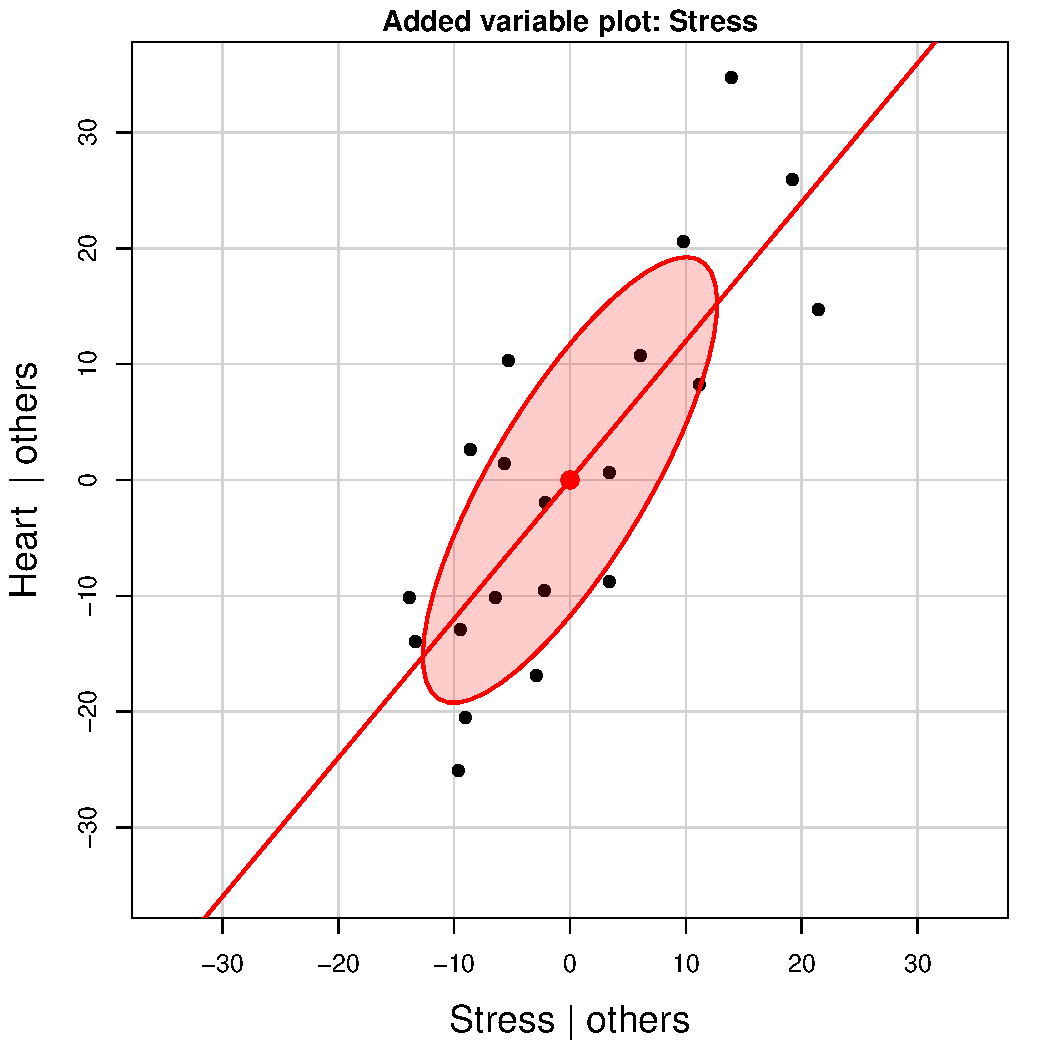
\includegraphics[width=1\linewidth]{fig/coffee-avplot1}
%  \caption{}%
%  \label{fig:}
 \end{minipage}%
 \hfill
 \begin{minipage}[b]{.49\linewidth}
  \centering
  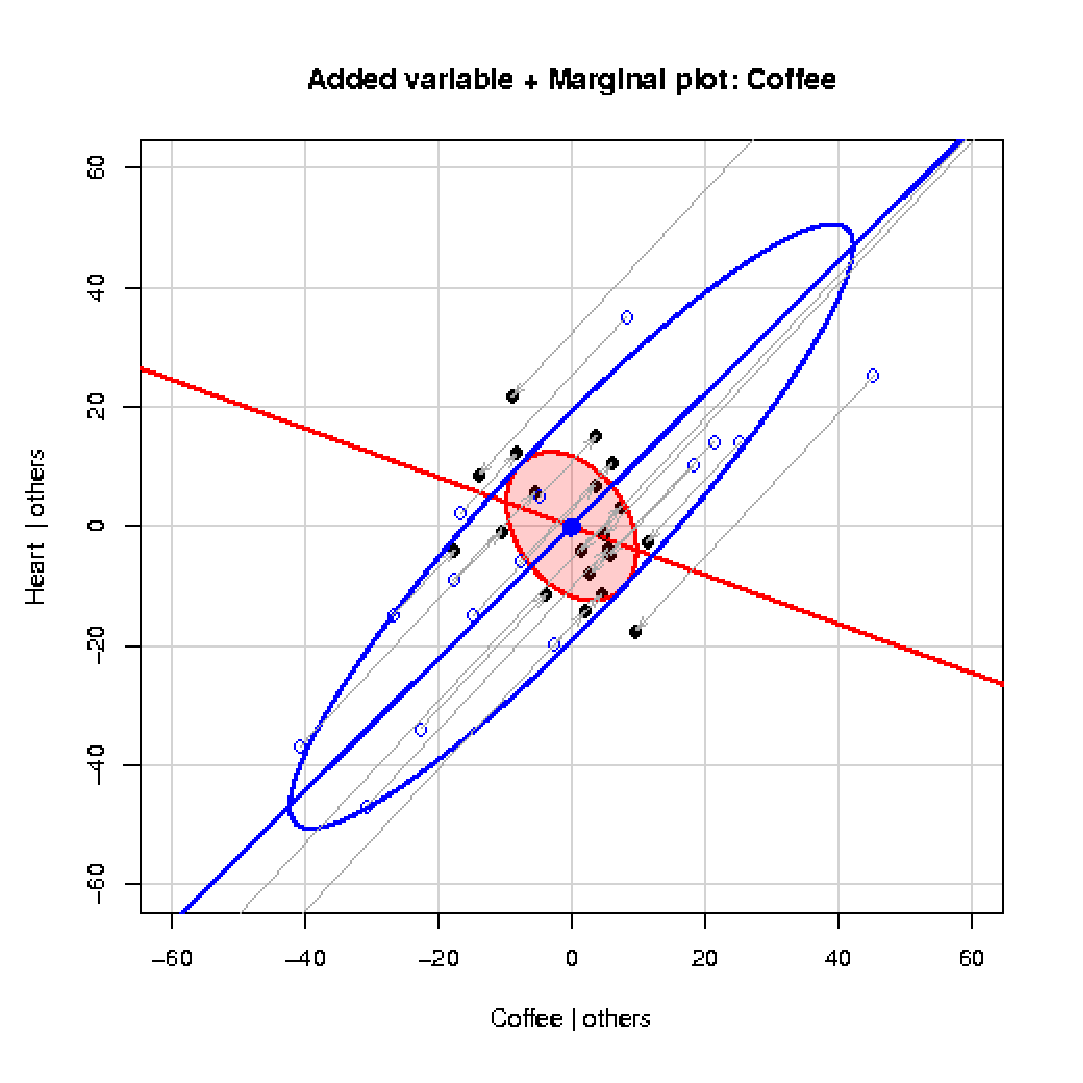
\includegraphics[width=1\linewidth]{fig/coffee-avplot2}
 \end{minipage}
  \caption{Added variable plots for Stress and Coffee in the multiple regression predicting Heart disease.
Each panel also shows the 50\% conditional data ellipse for residuals $(\vec{x}_k^\star, \vec{y}^\star)$, shaded red.
}
  \label{fig:coffee-avplot-A}
\end{figure}

Formally, we express the standard linear model in vector form as
$\widehat{\vec{y}} \equiv \widehat{\vec{y}} \given \mat{X} = \beta_0 \vec{1} + \beta_1 \vec{x}_1 + \beta_2 \vec{x}_2 + \dots +  \beta_p \vec{x}_p$,
with model matrix $\mat{X} = [ \vec{1}, \vec{x}_1, \dots \vec{x}_p ]$.
Let $\mat{X}_{[-k]}$ be the model matrix omitting the column for variable $k$.
Then algebraically, the added variable plot for variable $k$ is the scatterplot of the residuals $(\vec{x}^\star_k, \vec{y}^\star)$ from
two auxillary regressions, fitting $\vec{y}$ and $\vec{x}_k$ from $\mat{X}_{[-k]}$,
\begin{eqnarray*}
 \vec{y}^\star   & \equiv & \vec{y} \given \textrm{others}  =  \vec{y} - \widehat{\vec{y}} \given \mat{X}_{[-k]} \\
 \vec{x}^\star_k & \equiv & \vec{x}_k \given \textrm{others}  =  \vec{x}_k - \widehat{\vec{x}}_k \given \mat{X}_{[-k]}  \period \\
\end{eqnarray*}
(These quantities can all be computed \citep{VellemanWelsh:81} from the results of a single regression for the full model.)

Geometrically, in the space of the observations,\footnote{The ``space of the observations'' is yet a third, $n$-dimensional, space, in which the observations are the axes and each variable is represented as a point (or vector). See, e.g., \citet[Ch.~10]{Fox:2008}.} the fitted vector $\widehat{\vec{y}}$ is the orthogonal projection of $\vec{y}$
onto the subspace spanned by $\mat{X}$. Then $\vec{y}^\star$ and $\vec{x}^\star_k$ are the projections onto
the orthogonal complement of the subspace spanned by $\mat{X}_{[-k]}$, so
the simple regression of $\vec{y}^\star$ on $\vec{x}^\star_k$ has slope $\hat{\beta_k}$ in the full model,
and the residuals from the line $\vec{y}^\star = \hat{\beta_k} \vec{x}^\star_k$ in this plot are identically
the residuals from the overall regression of $\vec{y}$ on $\mat{X}$.

Another way to describe the added-variable plot (AVP) for $x_k$ is as a 2D projection of the space of
$(\vec{y}, \mat{X})$, viewed in the plane defined by the intersection of two hyperplanes:
the plane of the regression of $\vec{y}$ on all of $\mat{X}$, and the plane of regression of
$\vec{y}$ on $\mat{X}_{[-k]}$. A third plane, that of the regression of $x_k$ on $\mat{X}_{[-k]}$
also intersects in this space, and defines the horizontal axis in the AVP.
This is illustrated in \figref{fig:coffee-av3D}, showing one view defined by the intersection of
the three planes in the right panel.%
\footnote{Animated 3D movies of this plot are included among the supplementary materials for this paper.}

\begin{figure}[htb]
 \begin{minipage}[b]{.49\linewidth}
  \centering
  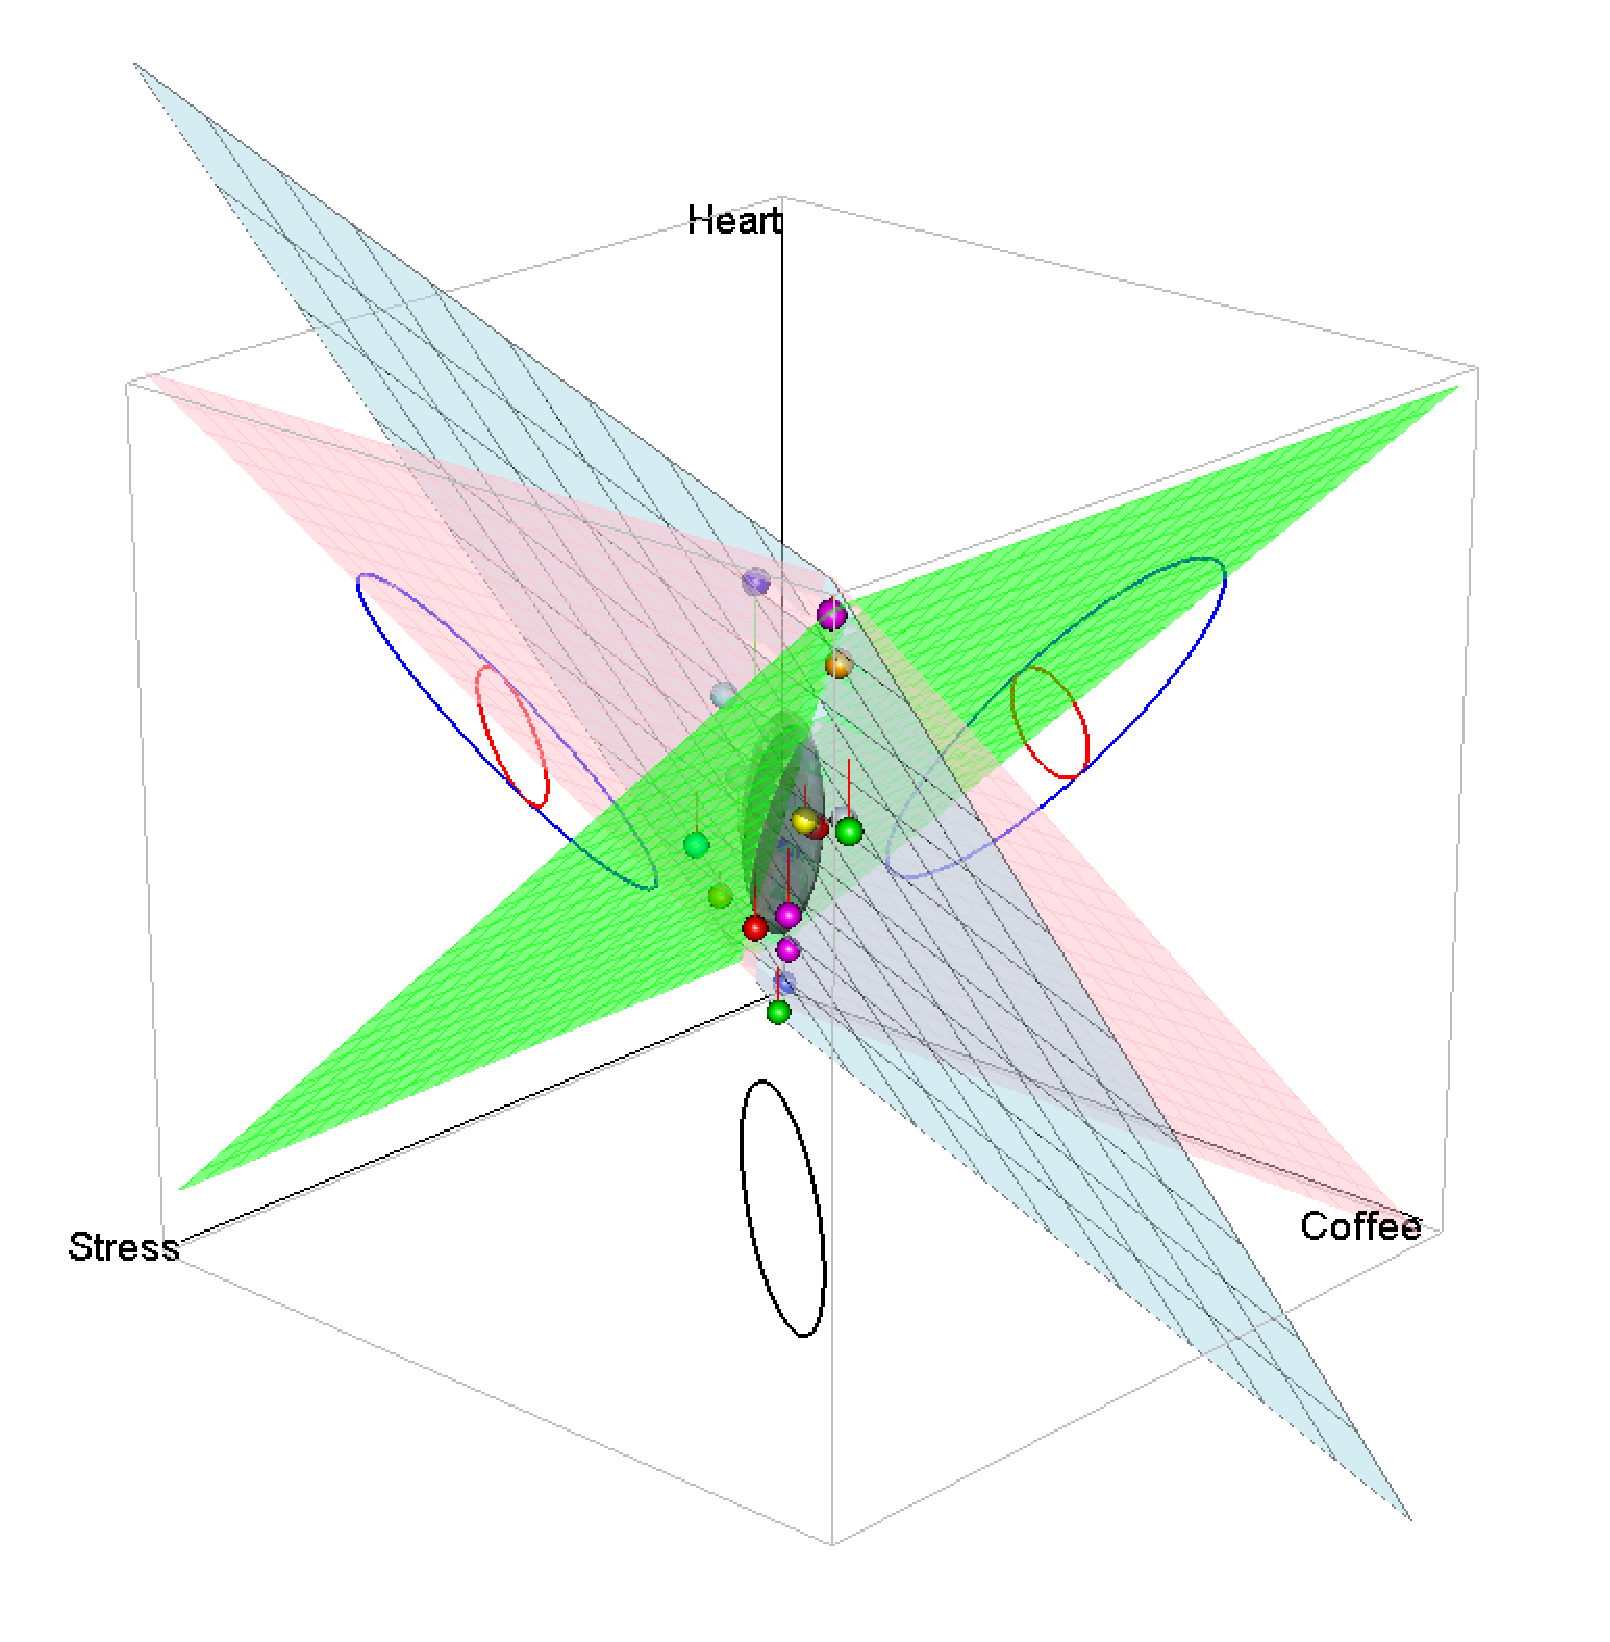
\includegraphics[width=1\linewidth]{fig/coffee-av3D-1}
%  \caption{}%
%  \label{fig:}
 \end{minipage}%
 \hfill
 \begin{minipage}[b]{.49\linewidth}
  \centering
  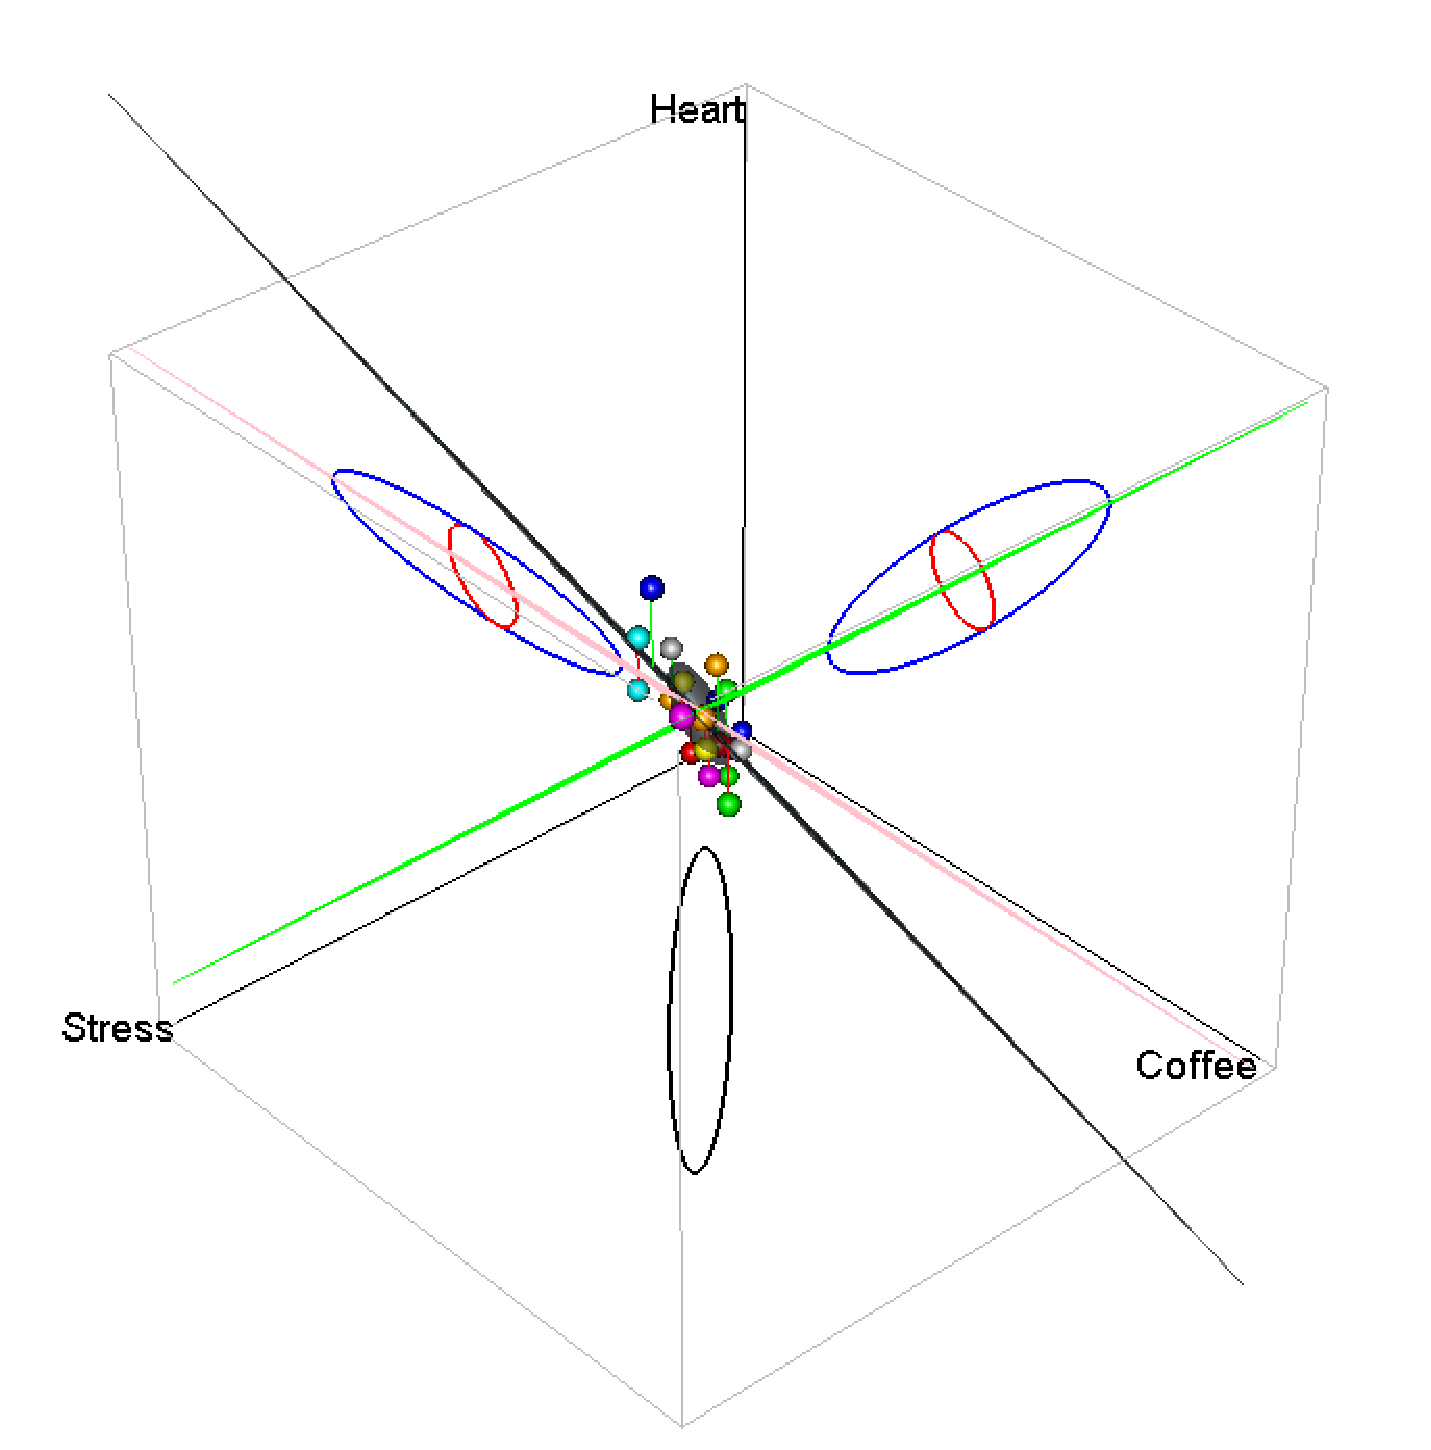
\includegraphics[width=1\linewidth]{fig/coffee-av3D-2}
 \end{minipage}
  \caption{3D views of the relationship between Heart, Coffee and Stress, showing the three regression planes
  for the marginal models, Heart $\sim$ Coffee (green), Heart $\sim$ Stress (pink), and the joint model, Heart $\sim$ Coffee $+$ Stress (light blue).
  Left: a standard view; right: a view showing all three regression planes on edge.
  The ellipses in the side panels are 2D projections of the standard conditional (red) and marginal (blue) ellipsoids, as shown in \figref{fig:coffee-avplot-B}.
  }
  \label{fig:coffee-av3D}
\end{figure}

%For three variables, $(y, x_1, x_2)$, the added variable plot for, say $x_1$, has particularly simple geometric interpretations in 3D in terms
%of the fitted planes for the full model, $y \sim x_1 + x_2$, the marginal model, $y \sim  x_2$

\figref{fig:coffee-avplot-A} shows added-variable plots for Stress and Coffee in the multiple regression predicting Heart disease,
supplemented by data ellipses for the residuals $(\vec{x}_k^\star, \vec{y}^\star)$.  With reference to the properties
of data ellipses in marginal scatterplots (see \figref{fig:ellipses-demo}), the following visual properties (among others)
are useful in this discussion.  These results follow simply from translating ``marginal'' into ``conditional'' (or ``partial'')
in the present context. 
The essential idea is that the data ellipse of the AVP for $(x_k, y)$ is to the estimate of a coefficient in a multiple regression as
 the data ellipse of $(x, y)$ is to simple regression. Thus:


\begin{figure}[htb]
 \begin{minipage}[b]{.49\linewidth}
  \centering
  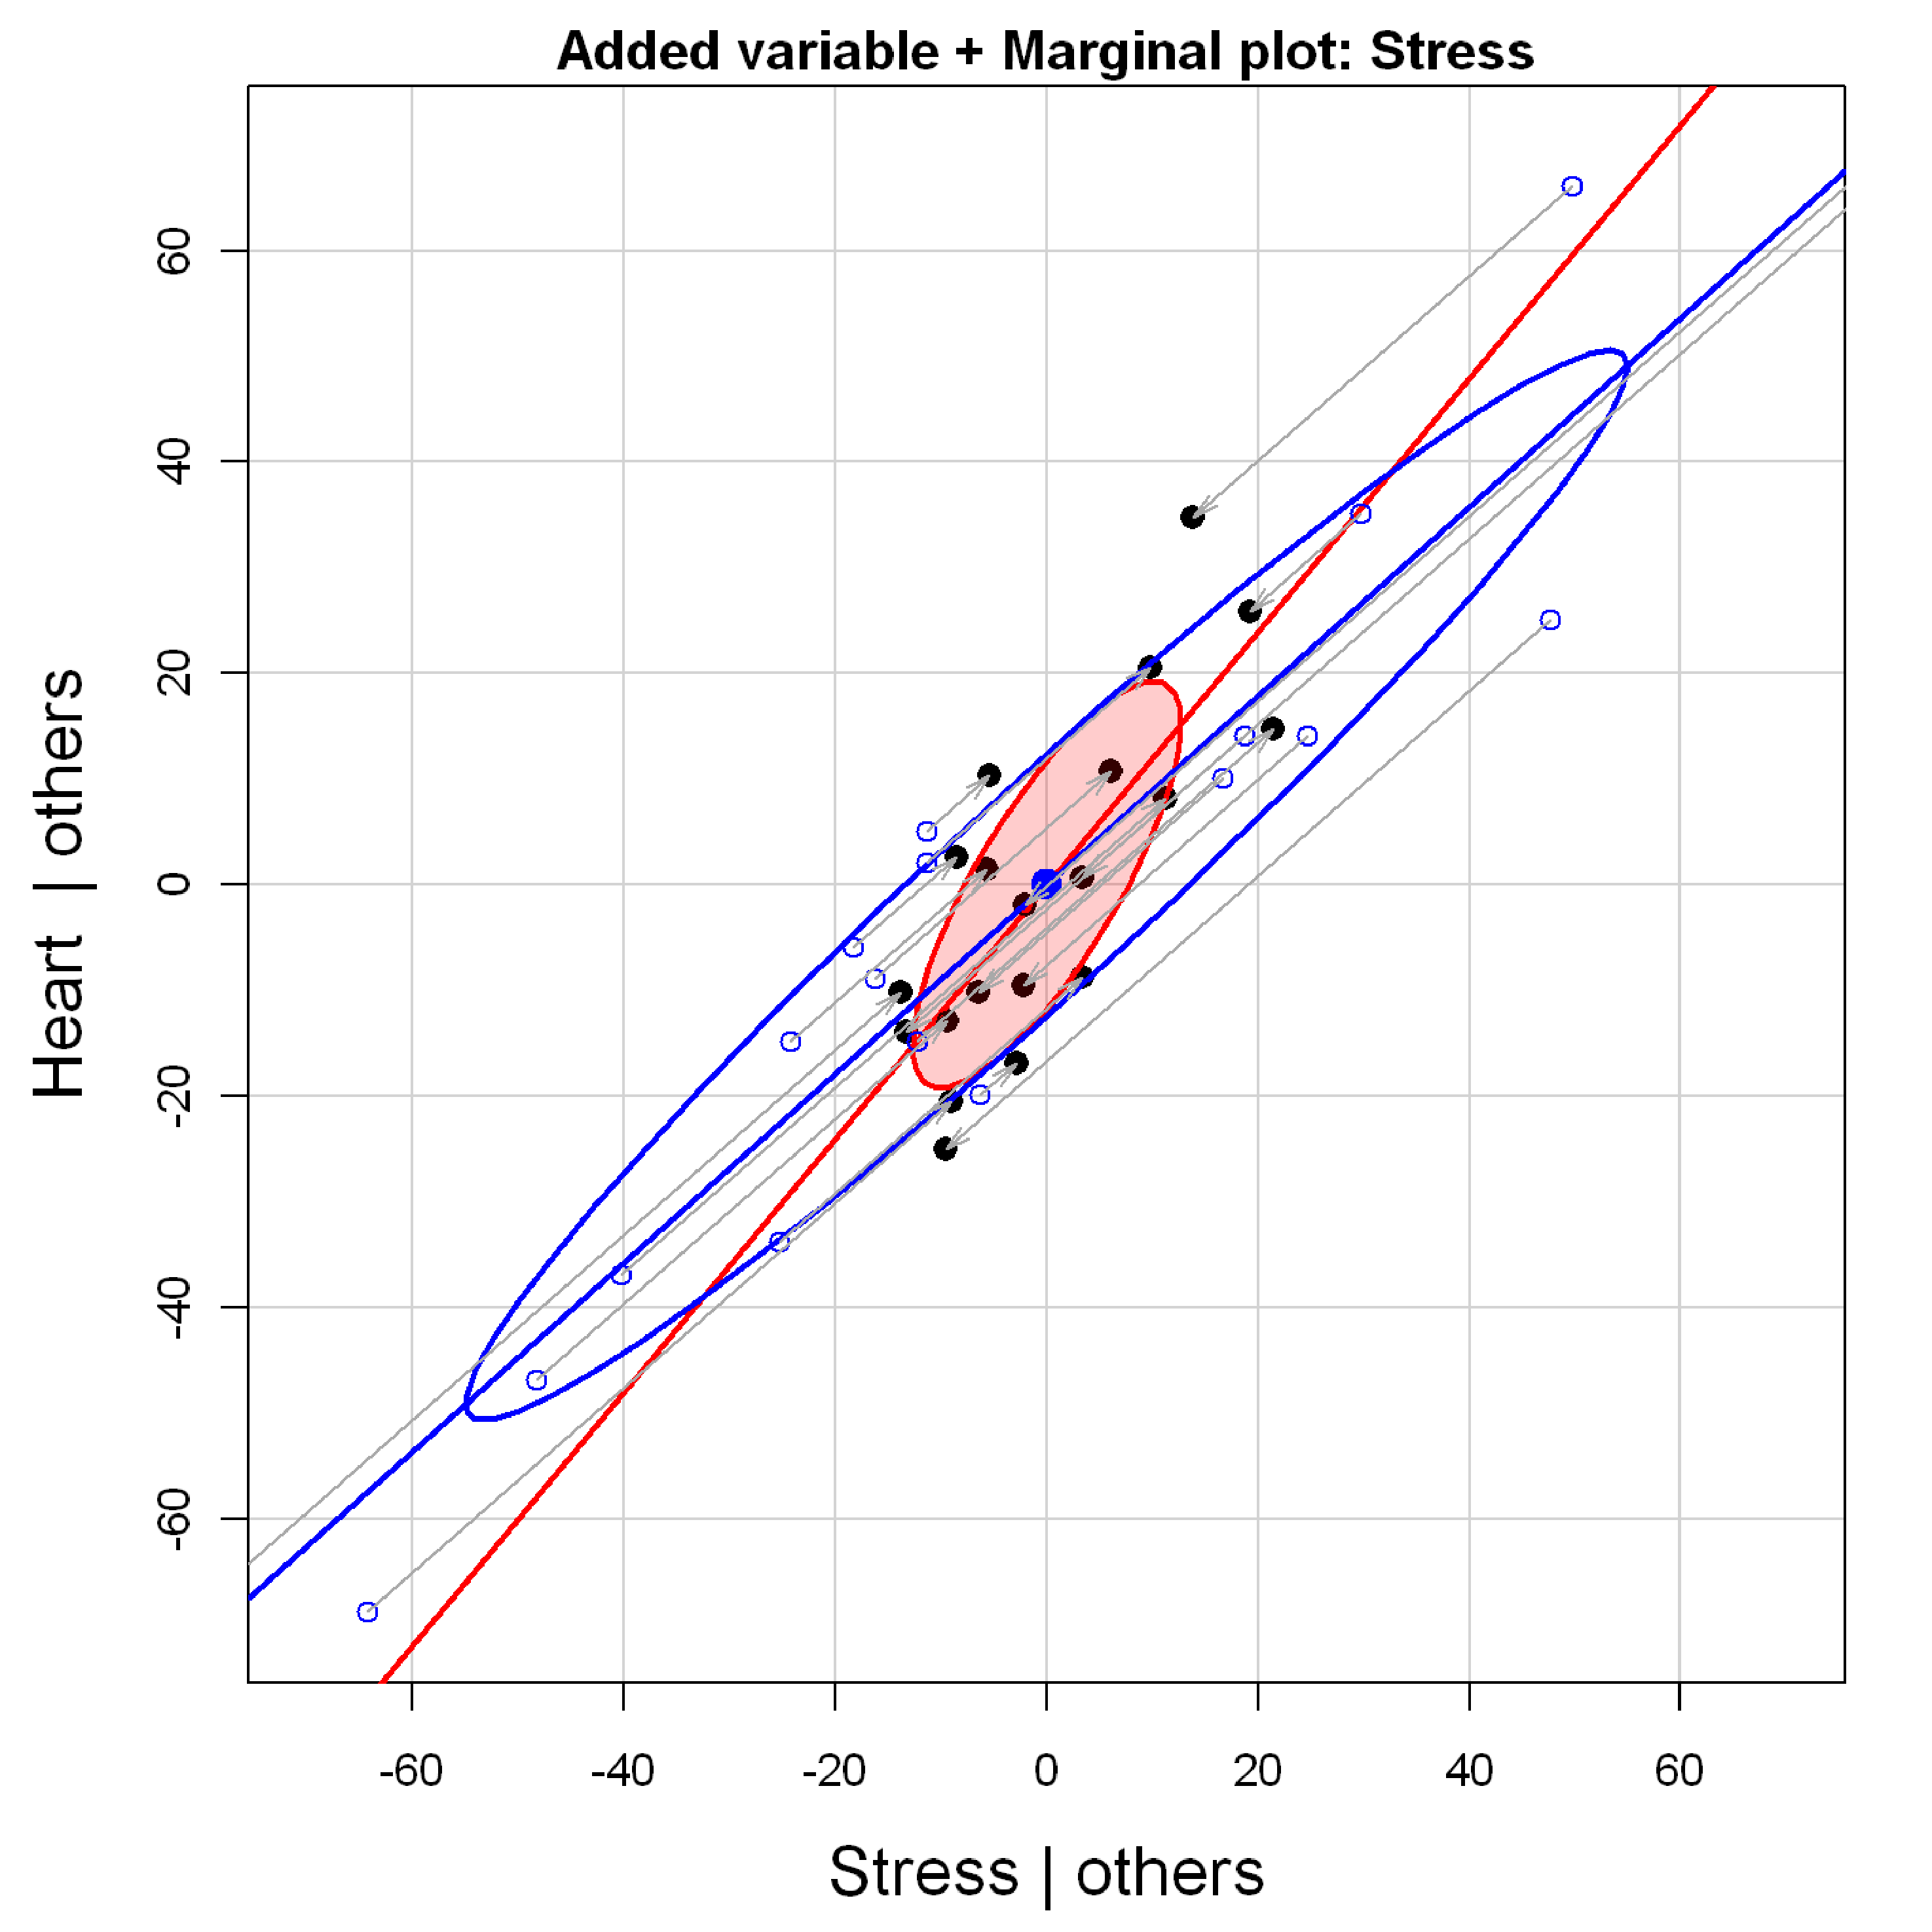
\includegraphics[width=1\linewidth]{fig/coffee-avplot3}
%  \caption{}%
%  \label{fig:}
 \end{minipage}%
 \hfill
 \begin{minipage}[b]{.49\linewidth}
  \centering
  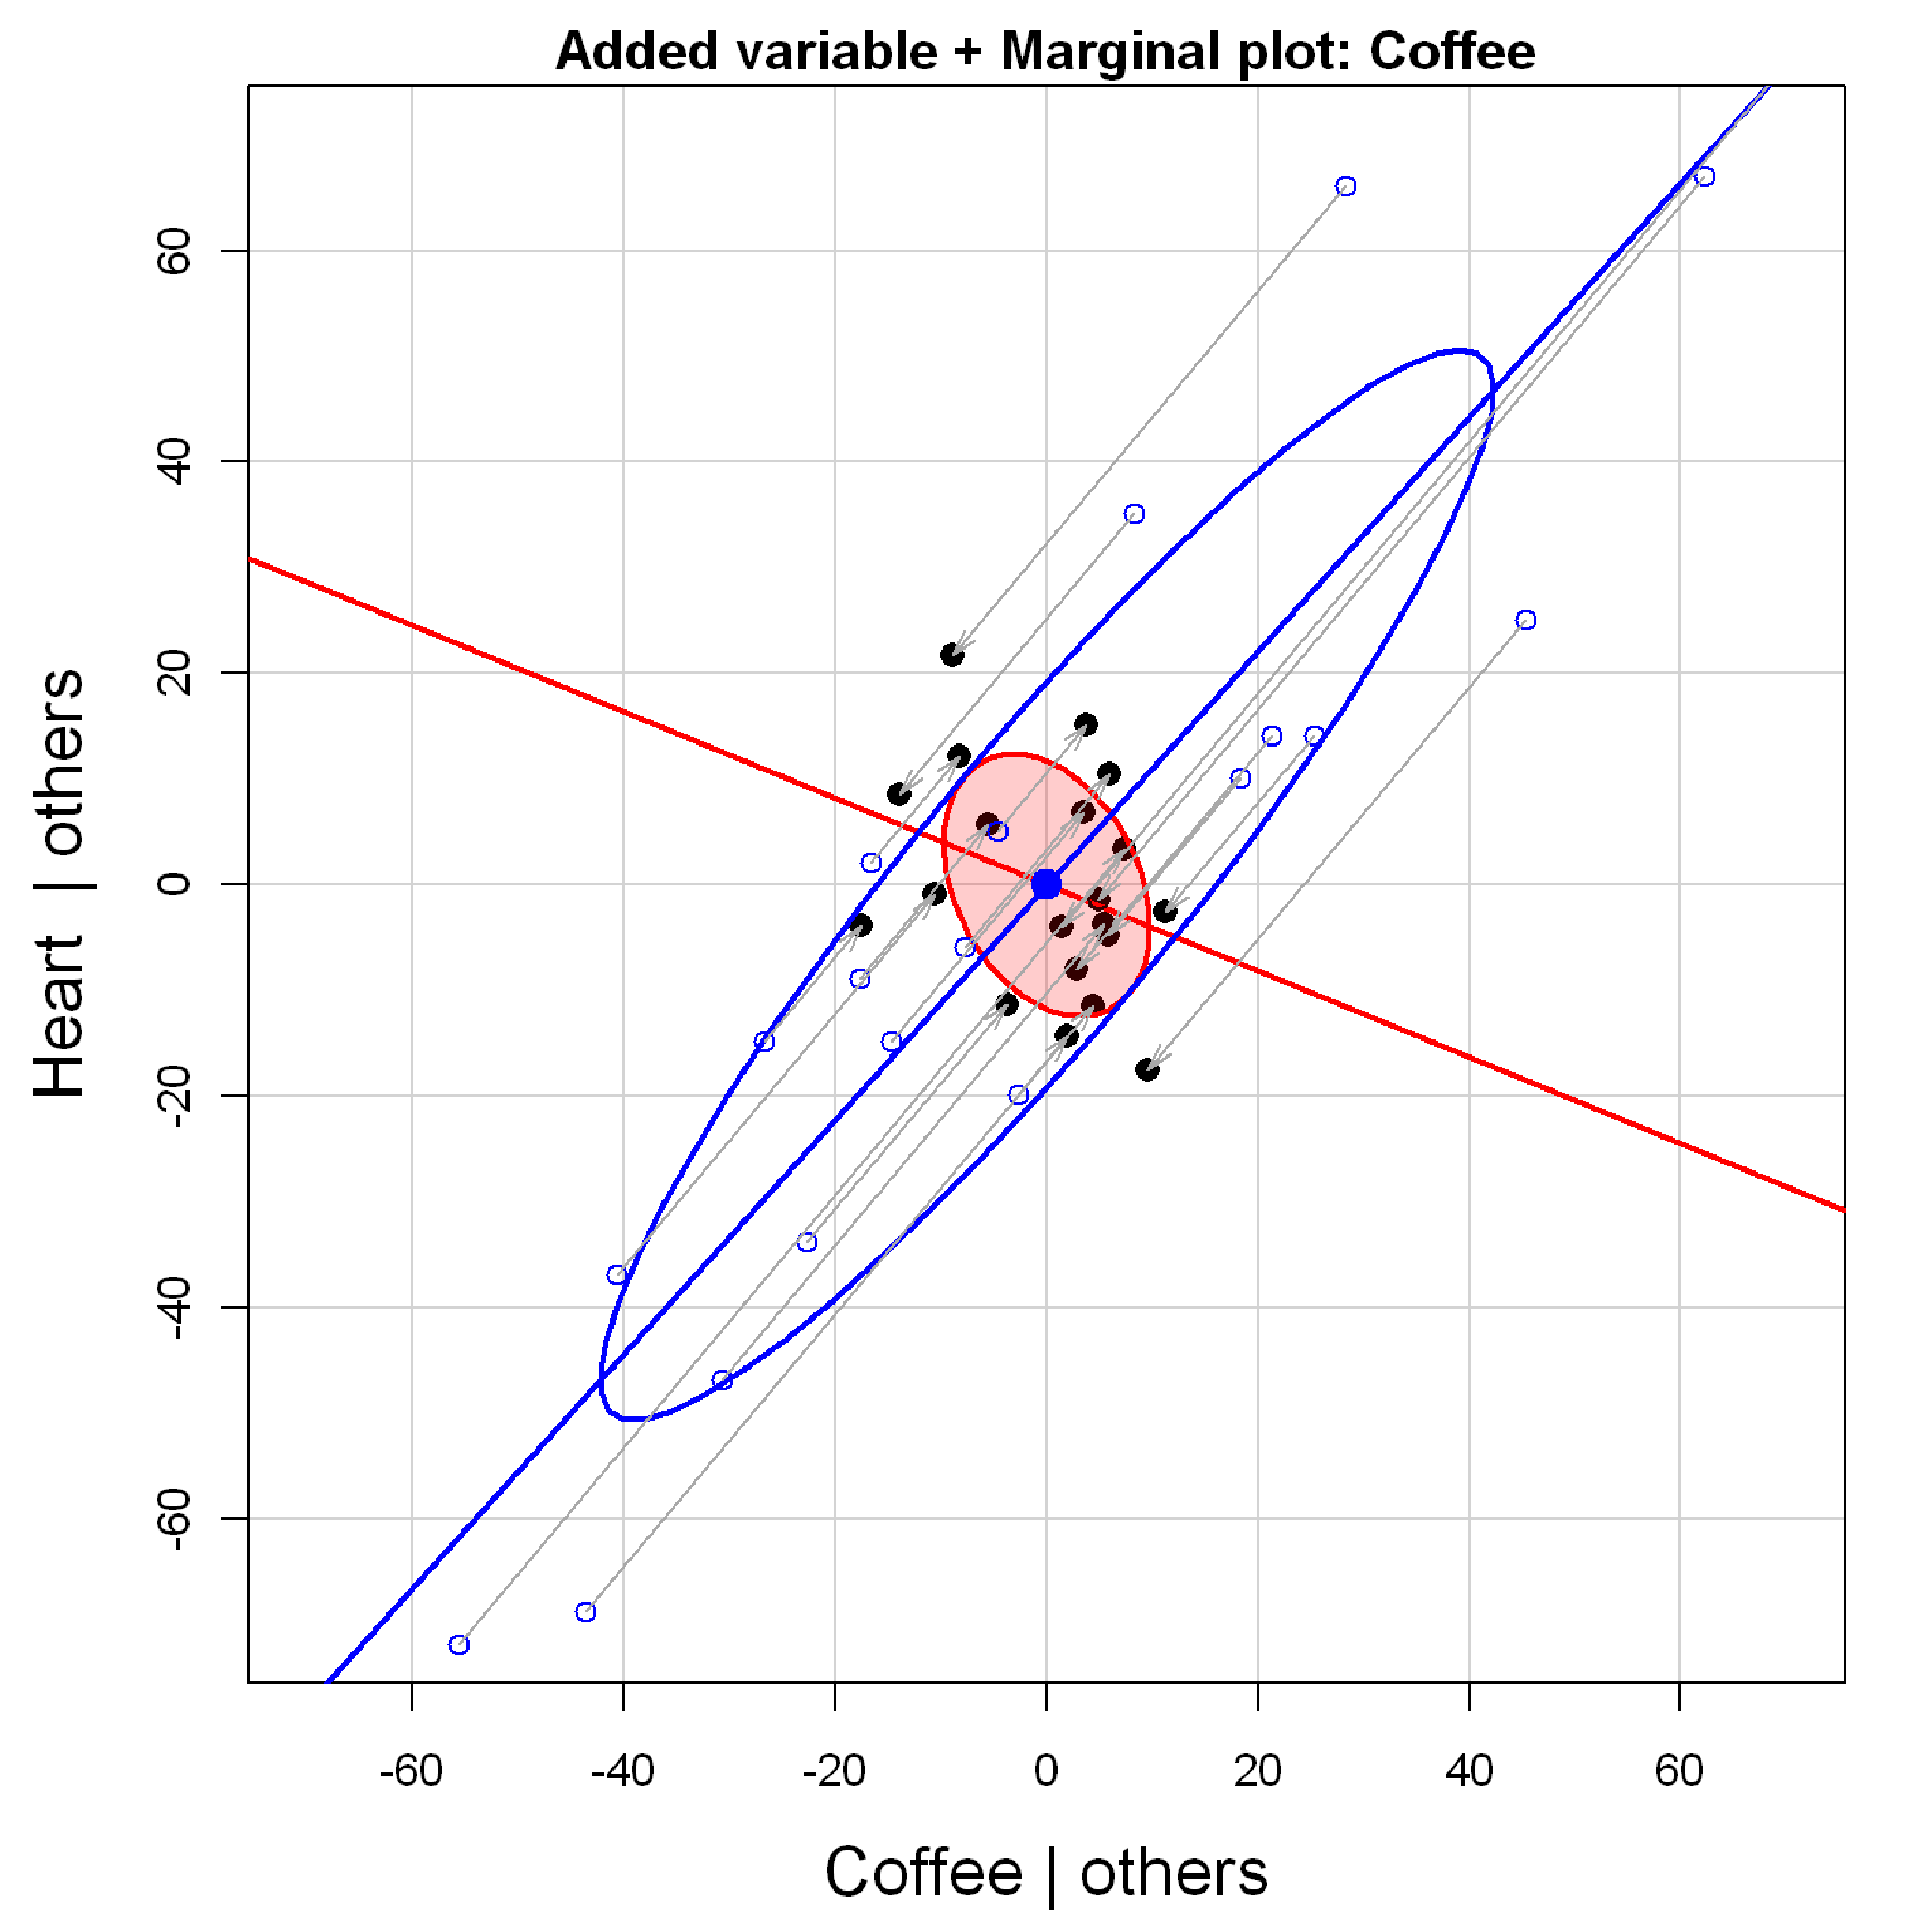
\includegraphics[width=1\linewidth]{fig/coffee-avplot4}
 \end{minipage}
  \caption{Added-variable $+$ marginal plots for Stress and Coffee in the multiple regression predicting Heart disease.
Each panel shows the 50\% conditional data ellipse for $x^{*}, y^{*}$ residuals (shaded, red) as well as the marginal 50\%
data ellipse for the $(x, y)$ variables, shifted to the origin.
Arrows connect the mean-centered marginal points (open circles) to the residual points (filled circles).}
  \label{fig:coffee-avplot-B}
\end{figure}

\begin{enumerate*}
%  \item The data ellipse of the AVP for $(x_k, y)$ is to the estimate of a coefficient in a multiple regression as
%  the data ellipse of $(x, y)$ is to simple regression. Thus:

 \item The simple regression least squares fit of $\vec{y}^\star$ on $\vec{x}_k^\star$ has slope $\hat{\beta_k}$,
 the partial slope for $x_k$ in the full model (and intercept = 0).

 \item The residuals, $(\vec{y}^\star - \widehat{\vec{y}}^\star)$, shown in this plot are the residuals for $\vec{y}$ in the full model.

 \item The correlation between $\vec{x}_k^\star$ and $\vec{y}^\star$, seen in the shape of the data ellipse for these residuals,
 is the partial correlation between $y$ and $x_k$ with the other predictors in $\mat{X}_{[-k]}$ partialled out.

 \item The horizontal half-width of the AVP data ellipse is proportional to the conditional standard deviation of
 $x_k$ remaining after all other predictors have been accounted for, providing a visual interpretation
 of variance inflation due to collinear predictors, as we describe below.

 \item The vertical half-width of the data ellipse is proportional to the residual standard deviation $s_e$ in the multiple regression.

 \item The squared horizontal positions, $(\vec{x}_k^\star)^2$, in the plot give the partial contributions
 to leverage on the coefficient $\hat{\beta}_k$ of $x_k$. 

 \item Items (3) and (7) imply that 
 that the AVP for $x_k$ shows the \emph{partial} influence of individual observations on the coefficient $\hat{\beta}_k$, 
 in the same way as in \figref{fig:levdemo21} for marginal models. These influence statistics are
 often shown numerically
 as DFBETA statistics \citep{Belsley-etal:80}.
 
 \item The last three items imply that the collection of added-variable plots for $\vec{y}$ and
 $\mat{X}$ provide an easy way to visualize the influence that individual observations---and indeed the joint influence of subsets of observations---have on
 the esimation of \emph{each} coefficient in a given model.
\end{enumerate*}


Elliptical insight also permits us to go further, to depict the relationship between conditional and marginal views
directly.
\figref{fig:coffee-avplot-B} shows the same added-variable plots for Heart disease on Stress and Coffee
as in \figref{fig:coffee-avplot-A} (with a zoomed-out scaling), but here we also overlay the
marginal data ellipses for $(x, y)$,
and and marginal regression lines for Stress and Coffee separately.  In 3D data space,
these are the shadows (projections) of the data ellipsoid onto the planes defined by the
partial variables.  In 2D AVP space, these are just the marginal data ellipses translated to
the origin.

The most obvious feature of \figref{fig:coffee-avplot-B} is that the AVP for Coffee has a negative slope in the conditional
plot (suggesting that controlling for Stress, coffee consumption is good for your heart), while
in the marginal plot increasing coffee seems to be bad for your heart. This serves as a
regression example of Simpson's paradox, which we considered earlier.

Less obvious is the fact that
the marginal and AVP ellipses are easily visualized as a shadow versus a slice of the full data ellipsoid.
Thus, the AVP ellipse must be contained in the marginal ellipse, as we can see in \figref{fig:coffee-avplot-B}.
If there are only two $x$s, then the AVP ellipse must touch the marginal ellipse at two points.
% This implies interesting contraints among the three quantities: improvement in fit, VIF, and change from marginal to conditional slope.
The shrinkage of the intersection of the AVP ellipse with the $y$ axis represents improvement in fit due to other $x$s.

More importantly, the shrinkage of the width (projected onto a horizontal axis) represents the
square root of the variance inflation factor (VIF), which can be shown to be the ratio of the horizontal
width of the marginal ellipse of $(x_k, y)$, with standard deviation $s(x_k)$ to the width of the conditional
ellipse of $(x_k^\star, y^\star)$, with standard deviation $s(x_k \given \textrm{others})$.
This geometry implies interesting contraints among the three quantities: improvement in fit, VIF, and change from the marginal to conditional slope.

Finally, \figref{fig:coffee-avplot-B} also shows how conditioning on other predictors works for individual
observations, where each point of  $(\vec{x}_k^\star, \vec{y}^\star)$ is the image of $(\vec{x}_k, \vec{y})$
along the path of the marginal regression. This reminds us that the AVP is a 2D projection of the full space,
where the regression plane of $\vec{y}$ on $\mat{X}_{[-k]}$ becomes the vertical axis and
the regression plane of $\vec{x}_k$ on $\mat{X}_{[-k]}$ becomes the horizontal axis.





%\section{Multivariate linear models: HE plots}\label{sec:mlm}

%\TODO{
%\begin{itemize*}
%\item H ellipse: data ellipse of fitted values; E ellipse: data ellipse of residuals [done]
%\item Visual tests of significance: Radii, volumes, etc
%\item Linear hypotheses: Geometries of contrasts and sums of effects
%\item Canonical projections; ellipses in data space and canonical space
%\end{itemize*}
%}

Multivariate linear models (\MLM{}s) have a special affinity with ellipsoids and elliptical geometry,
as described in this section.  To set the stage and establish notation, we consider
the \MLM\ (e.g., \citet{Timm:75}) given by
the equation $\mat{Y}=\mat{XB}+\mat{U}$, where $\mat{Y}$ is an $%
n\times p$ matrix of responses in which each column represents a distinct
response variable; $\mat{X}$ is the  $n\times q$ model matrix of full
column rank for the regressors; $\mat{\Beta}$ is the $q \times p$ matrix
of regression coefficients or model parameters; and $\mat{U}$ is the $n \times p$
matrix of errors,
with $\textrm{vec}(\mat{U}) \sim \mathcal{N}_p ( \mat{0}, \mat{I}_n \otimes \mat{\Sigma} )$,
where $\otimes$ is the Kronecker product.

A convenient feature of the \MLM\ for general multivariate responses is that
\emph{all} tests of linear hypotheses (for null effects) can be represented in the form of a general
linear test,
\begin{equation}\label{eq:mglt}
H_0: \sizedmat{L}{h \times q}
\sizedmat{\Beta}{q \times p} =
\sizedmat{0}{h \times p}
\comma
\end{equation}
where $\mat{L}$ is a rank $h \leq q$ matrix of constants whose rows specify
$h$ linear combinations or contrasts
of the parameters to be tested simultaneously
by a multivariate test.

For \emph{any} such hypothesis of the form given in \eqref{eq:mglt}, the analogs of the univariate
sums of squares for hypothesis ($\mathrm{SS}_H$) and error ($\mathrm{SS}_E$)
are the $p \times p$  sum of squares and cross-products (SSP) matrices given by:
\begin{equation} \label{eq:hmat}
\mat{H}  \equiv \mat{SSP}_H =
 (\mat{L} \widehat{\mat{B}})\trans \,
 [\mat{L} (\mat{X}\trans \mat{X} )^{-} \mat{L}\trans]^{-1} \,
 (\mat{L} \widehat{\mat{B}})
 \comma
\end{equation}
and
\begin{equation} \label{eq:emat}
\mat{E}  \equiv \mat{SSP}_E =
 \mat{Y}\trans \mat{Y} -
 \widehat{\mat{B}}\trans (\mat{X}\trans \mat{X}) \widehat{\mat{B}}
 =
  \widehat{\mat{U}}\trans  \widehat{\mat{U}}
 \comma
\end{equation}
where $\widehat{\mat{U}} = \mat{Y} - \mat{X} \widehat{\mat{B}}$ is the matrix of residuals.
Multivariate test statistics (Wilks's $\Lambda$, Pillai trace, Hotelling-Lawley trace, Roy's maximum root)
for testing \eqref{eq:mglt} are based on the $s = \min(p, h)$ non-zero latent roots
$\lambda_{1}>\lambda_{2}>\cdots>\lambda_{s}$ of
the matrix \mat{H} relative to the matrix \mat{E}, that is,
the values of $\lambda$ for which $
\det{\mat{H}-\lambda\mat{E}}=0$, or equivalently
the latent roots $\rho_i$ for which $\detbracket{\mat{H} - \rho (\mat{H}+\mat{E})}=0$.
The details are shown in \tabref{tab:criteria}.
% but note that $\rho_i = \lambda_i / (1+\lambda_i)$ 
These measures
attempt to capture how ``large'' $\mat{H}$ is, relative to
$\mat{E}$ in $s$ dimensions, and correspond to various ``means'' as we described earlier.
All of these statistics have transformations to $F$ statistics
giving either exact or approximate null-hypothesis $F$ distributions.
The corresponding latent vectors provide a
set of $s$ orthogonal linear combinations of the responses that produce
maximal univariate $F$ statistics for the hypothesis in \eqref{eq:mglt};
we refer to these as the \emph{canonical discriminant} dimensions.


\begin{table}[htb]
\renewcommand{\arraystretch}{1.6}
\caption{Multivariate test statistics as functions of the eigenvalues $\lambda_i$ solving $\det{\mat{H} - \lambda \mat{E}}=0$
or eigenvalues $\rho_i$ solving  $\detbracket{\mat{H} - \rho (\mat{H}+\mat{E})}=0$.
}\label{tab:criteria}
\begin{center}
\begin{tabular}{|l|l|l|l|}
  \hline
  % after \\: \hline or \cline{col1-col2} \cline{col3-col4} ...
  Criterion & Formula & ``mean'' of $\rho$ & Partial $\eta^2$   \\
  \hline
  Wilks's $\Lambda$ & $\Lambda = \prod^s_i \frac{1}{1+\lambda_i} = \prod^s_i (1-\rho_i)$ & geometric & $\eta^2 = 1-\Lambda^{1/s}$   \\
  Pillai trace & $V = \sum^s_i \frac{\lambda_i}{1+\lambda_i} = \sum^s_i \rho_i$ & arithmetic & $\eta^2 = \frac{V}{s} $   \\
  Hotelling-Lawley trace & $H = \sum^s_i \lambda_i = \sum^s_i \frac{\rho_i}{1-\rho_i} $ & harmonic & $\eta^2 = \frac{H}{H+s}$   \\
  Roy maximum root & $R = \lambda_1 = \frac{\rho_1}{1-\rho_1}$  & supremum & $ \eta^2 = \frac{\lambda_1}{1+\lambda_1} = \rho_1$   \\
  \hline
\end{tabular}
\end{center}
\end{table}
%\end{document}


%% added by GM; edited by MF
Beyond the informal characterization of the four classical tests of hypotheses for multivariate linear 
models given in
\tabref{tab:criteria}, there is an interesting geometrical representation 
that helps one to appreciate their relative power for various alternatives.  
%Let $\mat{H}$ be a hypothesis sums of squares and cross-products matrix,  
%$\mat{H}=(\mat{L}\hat{\mat{B}}-\mat{C})\trans (L(X\trans X)^{-1}L\trans )^{-1}(\mat{L}\hat{\mat{B}}-\mat{C})$ and let $\mat{E}$ be the residual sum of squares and cross-products matrix.
%Letting $\mat{\Lambda}$ be defined as it was above, 
This can be illustrated most simply in terms of 
the canonical representation,  $(\mat{H}+\mat{E})^\star$,
of the ellipsoid generated by $(\mat{H} + \mat{E})$ relative to $\mat{E}$,
as shown in \figref{fig:mtests} for $p=2$. 

\begin{figure}[htb]
  \centering
  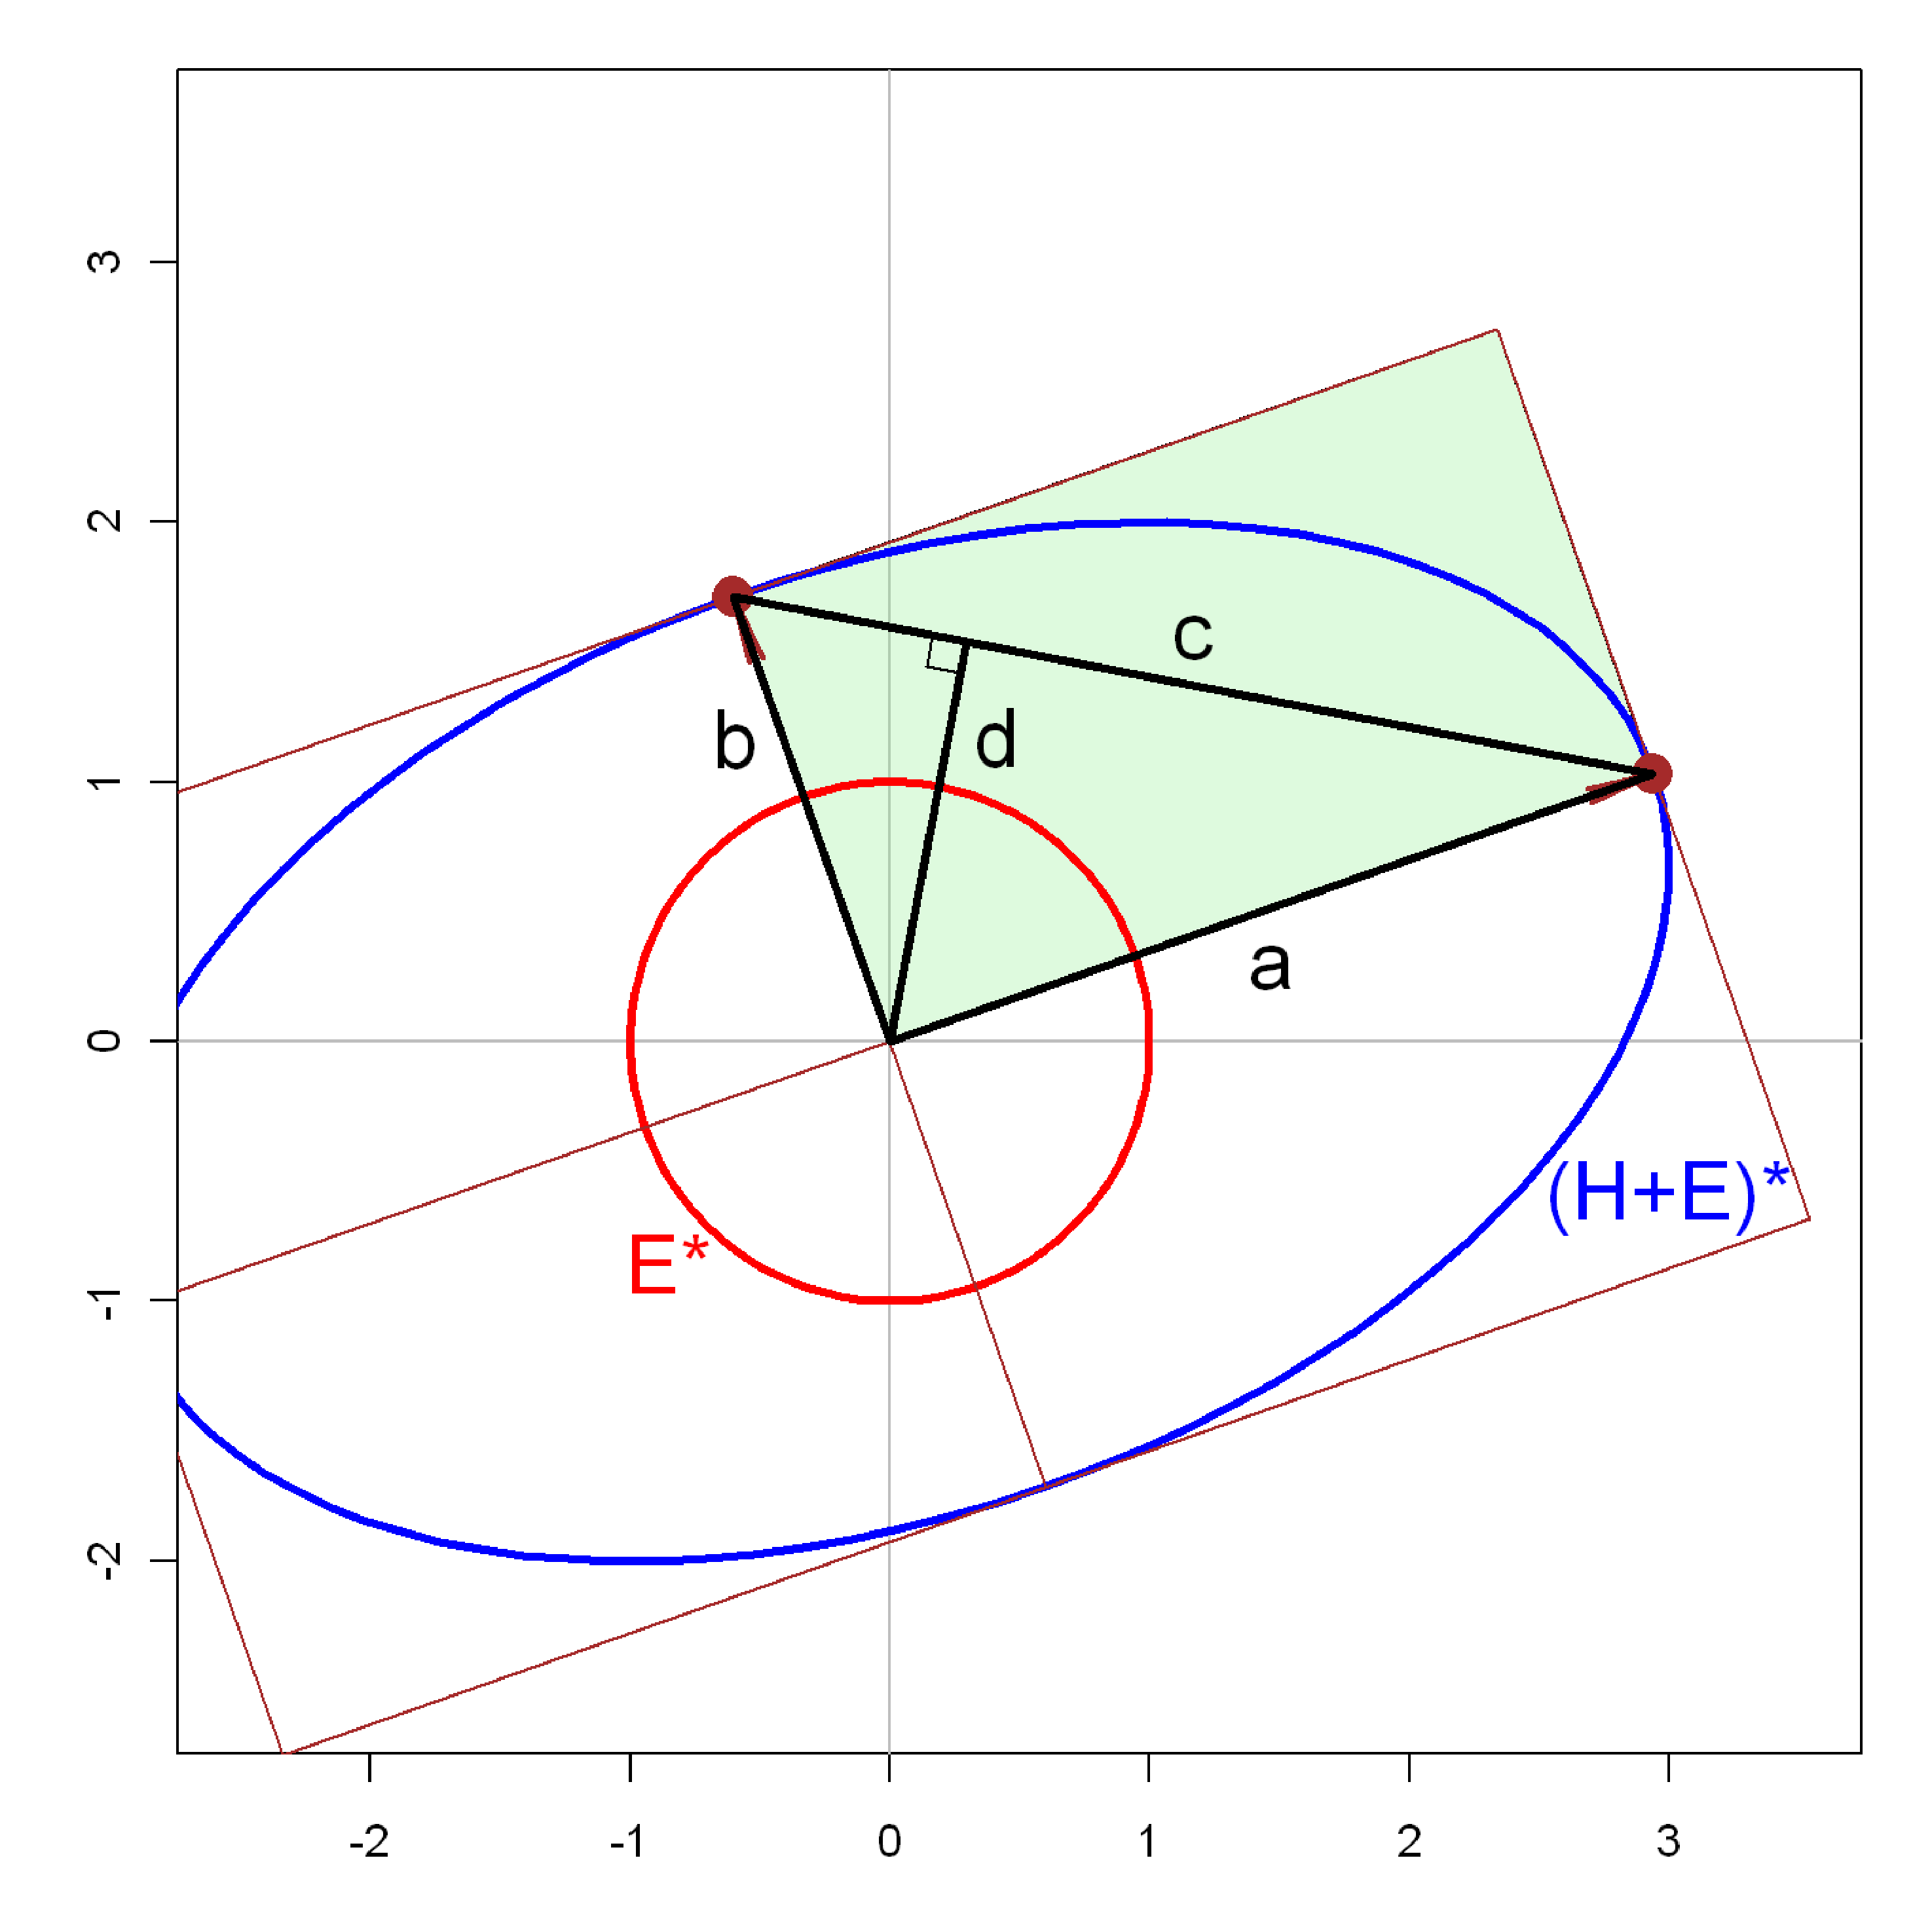
\includegraphics[width=.5\textwidth,clip]{fig/mtests}
  \caption{Geometry of the classical test statistics used in tests of hypotheses in multivariate linear models.
  The figure shows the representation of the ellipsoid generated by $(\mat{H} + \mat{E})$ relative to $\mat{E}$
  in canonical space where $\mat{E}^\star = \mat{I}$ and $(\mat{H}+\mat{E})^\star$ is the corresponding transformation
  of $(\mat{H} + \mat{E}).$
  }%
  \label{fig:mtests}
\end{figure}

With $\lambda_i$ as described above, 
the eigenvalues and squared radii of $(\mat{H}+\mat{E})^\star$ are $\lambda_i + 1$,
so the lengths of the major and minor axes are  $a=\sqrt{\lambda_1 + 1}$ and $b=\sqrt{\lambda_2 + 1}$ respectively.
The diagonal of the triangle comprising the segments $a, b$ (labelled $c$) has length
$c = \sqrt{a^2 + b^2}$.
Finally, a line segment from the origin dropped perpendicularly to the diagonal joining the two ellipsoid axes is labelled $d$.

In these terms, 
Wilks's test, based on $\prod{(1+\lambda_i)^{-1}}$ is equivalent to a test based on
$a \times b$ which is proportional to the area of the framing rectangle, shown shaded in \figref{fig:mtests}.
The Hotelling-Lawley trace test, based on
$\sum{\lambda_i}$ 
is equivalent to a test based on 
$c=\sqrt{\sum{\lambda_i} + p}$.
Finally, the Pillai Trace test, based on $\sum{\lambda_i (1+\lambda_i)^{-1}}$  can be shown to be equal to 
$2-d^{-2}$ for $p=2$. Thus it is strictly monotone in $d$ and equivalent to a test based directly on $d$.
%% see proof at http://scs.math.yorku.ca/index.php/General_Linear_Models/Visualizing_Multivariate_Tests

The geometry makes it easy to see that if there is a large discrepancy between $\lambda_1$ and $\lambda_2$, Roy's test depends 
only on $\lambda_1$ 
while the Pillai test depends more on $\lambda_2$. 
Wilks's $\Lambda$ and the Hotelling-Lawley trace criterion are also functional averages of $\lambda_1$ and $\lambda_2$, with the 
former being penalized when $\lambda_2$ is small.  In practice, when $s \le 2$, all four test criteria are equivalent, in that
their standard transformations to $F$ statistics are exact and give rise to identical $p$-values.



\subsection{Hypothesis-Error (HE) plots}

The essential idea behind HE plots is that any multivariate hypothesis
test, \eqref{eq:mglt}, can be represented visually by ellipses (or ellipsoids beyond 2D) that express
the size  of covariation against a multivariate null hypothesis
($\mat{H}$) relative to error covariation ($\mat{E}$).
The multivariate tests, based on the latent roots of $\mat{H} \mat{E}^{-1}$,
are thus translated directly to the sizes of the \mat{H} ellipses for
various hypotheses, relative to the size of the \mat{E} ellipse.
Moreover, the shape and orientation of these ellipses show something more---the
directions (linear combinations of the responses) that lead to
various effect sizes and significance.

\begin{figure}[htb]
  \centering
  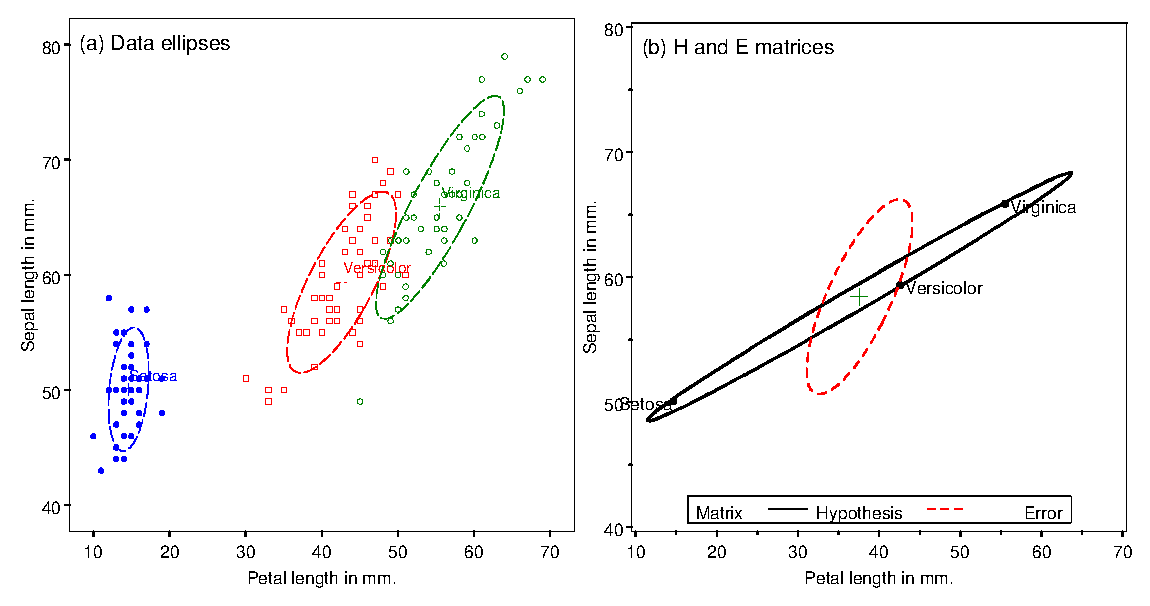
\includegraphics[width=.9\textwidth,clip]{fig/heplot3a}
  \caption{(a) Data ellipses and (b) corresponding HE plot for sepal length and petal length in the iris dataset.
  	The \mat{H} ellipse is the data ellipse of the fitted values defined by the group means, $\bar{\vec{y}}_{i \cdot}$
  	The \mat{E} ellipse is the data ellipse of the residuals, $(\vec{y}_{ij} - \bar{\vec{y}}_{i \cdot})$.
  	Using evidence (``significance'') scaling of the \mat{H} ellipse, the plot has the property that
  	the multivariate test for a given hypothesis is significant by Roy's largest-root test \emph{iff}
  	the \mat{H} ellipse protrudes anywhere outside the \mat{E} ellipse.}%
  \label{fig:heplot3a}
\end{figure}

\figref{fig:heplot3a} illustrates this idea for two variables from the iris dataset.
Panel (a) shows the data ellipses for sepal length and petal length, equivalent to
the corresponding plot in \figref{fig:scatirisd1}. Panel (b) shows the HE plot for these
variables from the one-way MANOVA model $\vec{y}_{ij} = \vec{\mu}_i + \vec{u}_{ij}$
testing equal mean vectors across species, $H_0: \vec{\mu}_1 = \vec{\mu}_2 = \vec{\mu}_3$.
Let $\widehat{\mat{Y}}$ be the $n \times p$ matrix of fitted values for this model,
i.e., $\widehat{\mat{Y}} = \{ \bar{\vec{y}}_{i \cdot} \}$.
Then $\mat{H}= \widehat{\mat{Y}}\trans \widehat{\mat{Y}} - n\bar{\vec{y}} \bar{\vec{y}}\trans $ (where $\bar{\vec{y}}$ is the grand-mean vector), and the \mat{H} ellipse in the figure is then just the
2D projection of the data ellipsoid
of the fitted values, scaled as described below.
Similarly, $\widehat{\mat{U}} = \mat{Y} - \widehat{\mat{Y}}$, and
$\mat{E} = \widehat{\mat{U}}\trans  \widehat{\mat{U}} = (N-g) \mat{S}_{\mathrm{pooled}}$, so the \mat{E} ellipse is
the 2D projection of the data ellipsoid of the residuals.
Visually, the \mat{E} ellipsoid corresponds to shifting the separate within-group data ellipsoids to the centroid,
as illustrated above in \figref{fig:contiris3}(c).

In HE plots, the \mat{E} matrix is first scaled to a covariance matrix
$\mat{E}/df_e$, dividing by the error degrees of freedom, $df_e$.
The ellipsoid drawn is
translated to the centroid $\overline{\vec{y}}$ of the variables,
giving $\overline{\vec{y}} \oplus c \mat{E}^{1/2}/df_e$.
This scaling and translation
also allows the means for levels of the factors
to be displayed in the same space,
facilitating interpretation.
In what follows, we show these as
``standard'' bivariate ellipses of 68\% coverage,
using $c=\sqrt{2 F_{2, df_e}^{.68}}$, except where noted otherwise.

The ellipse for \mat{H} reflects the size and orientation of covariation
against the null hypothesis.
In relation to the \mat{E} ellipse, the \mat{H} ellipse
can be scaled to show either the \emph{effect size} or strength of
\emph{evidence} against $H_0$ (significance).

For effect-size scaling, each \mat{H} is divided by $df_e$ to conform
to \mat{E}.  The resulting ellipse is then exactly the data ellipse
of the fitted values, and corresponds visually to a multivariate analog of
univariate effect-size measures (e.g., $(\bar{y}_1 - \bar{y}_2)/s_e$
where $s_e$ is the within-group standard deviation).

For significance scaling, it turns out to be most visually convenient to
use Roy's largest-root statistic as the test criterion.
In this case,
the \mat{H} ellipse is scaled to $\mat{H}/(\lambda_\alpha df_e)$
where $\lambda_\alpha$ is the critical value of Roy's statistic.%
\footnote{
The $F$ test based on Roy's largest root uses the approximation
$ F = (df_2 / df_1) \lambda_1$ with degrees of freedom $df_1, df_2$,
where $df_1 = \max (df_h, df_e)$ and $df_2 = df_e - df_1 + df_h$.
Inverting the $F$ statistic gives the critical value for an $\alpha$-level test:
$\lambda_\alpha = (df_1/df_2) F^{1-\alpha}_{df_1,df_2}$
}
Using this scaling gives a simple visual test of
$H_0$: Roy's test rejects $H_0$ at a given $\alpha$ level \emph{iff}
the corresponding $\alpha$-level \mat{H} ellipse protrudes \emph{anywhere} outside the \mat{E}
ellipse.%
\footnote{Other multivariate tests (Wilks's $\Lambda$, Hotelling-Lawley trace,
Pillai trace) also have geometric interpretations
in HE plots (e.g.,  Wilks's $\Lambda$ is the ratio of areas (volumes)
of the \mat{H} and \mat{E} ellipses (ellipsoids); Hotelling-Lawley trace
is based on the sum of the $\lambda_i$), but these statistics do not provide
such simple visual comparisons. All HE plots shown in this paper use
significance scaling, based on Roy's test.
}
Moreover, the directions in which the hypothesis ellipse exceed the error ellipse
are informative about the responses and their linear combinations that depart significantly
from $H_0$.  Thus, in \figref{fig:heplot3a}(b), the variation of the means of the iris species
shown for these two variables
appears to be largely one-dimensional, corresponding to a weighted sum (or average) of petal length and
sepal length, perhaps a measure of overall size.


\subsection{Linear hypotheses: geometries of contrasts and sums of effects}

Just as in univariate ANOVA designs, important overall effects ($\textrm{df}_h>1$) in MANOVA may be usefully
explored and interpreted by the use of contrasts among the levels of the factors involved.
In the general linear hypothesis test of \eqref{eq:mglt}, contrasts are easily specified as one or more $(h_i \times q)$ \mat{L}
matrices, $\mat{L}_1, \mat{L}_2, \dots $, each of whose rows sums to zero.

As an important special case,
for an overall effect with
$\textrm{df}_h$ degrees of freedom (and balanced sample sizes), a set of $\textrm{df}_h$ pairwise orthogonal $(1 \times q)$
\mat{L} matrices ($\mat{L}_i \trans \mat{L}_j =0$ for $i\ne j$) gives rise to a set of $\textrm{df}_h$ rank-one $\mat{H}_i$
matrices that additively decompose the overall hypothesis SSCP matrix (by a multivariate analog of Pythagoras' Theorem),
\begin{equation*}
\mat{H} = \mat{H}_1 + \mat{H}_2 + \cdots + \mat{H}_{\textrm{df}_h}
\comma
\end{equation*}
exactly as the univariate $SS_H$ may be decomposed in an ANOVA.  Each of these rank-one $\mat{H}_i$ matrices
will plot as a vector in an HE plot, and their collection provides a visual summary of the overall
test, as partitioned by these orthogonal contrasts.
Even more generally, where the subhypothesis matrices may be of rank $>$ 1,  the subhypotheses will have hypothesis ellipses of dimension rank($\mat{H}_i$)
that are conjugate with respect to the hypothesis ellipse for the joint hypothesis, provided that the
estimators for the subhypotheses are statistically independent.

\fig{HE-contrasts-iris}{width=.6\textwidth,clip}{$\mat{H}$ and $\mat{E}$ matrices for sepal width and sepal length in the iris
data, together with $\mat{H}$ matrices for testing two orthogonal contrasts in the species effect.}

To illustrate, we show in \figref{fig:HE-contrasts-iris} an HE plot for the sepal width and sepal length variables in the iris data,
corresponding to panel (1:2) in \figref{fig:scatirisd1}. Overlayed on this plot are the
one-df \mat{H} matrices obtained from testing two orthogonal contrasts among the iris species:
\emph{setosa} vs.\ the average of \emph{versicolor} and \emph{virginica} (labeled ``S:VV''), and \emph{versicolor} vs. \emph{virginica} (``V:V''), for which the contrast matrices are
\begin{eqnarray*}
\mat{L}_1 & = &
( \begin{array}{rrr}
-2 & 1 & 1
\end{array} )
\\
\mat{L}_2 & = &
( \begin{array}{rrr}
0 & 1 & -1
\end{array} ) \comma
\end{eqnarray*}
where the species (columns) are taken in alphabetical order. In this view, the joint hypothesis testing
equality of the species means has its major axis in data space largely in the direction of sepal length.
The 1D degenerate ``ellipse'' for $\mat{H}_1$, representing the contrast of setosa with the average of the other two species,
is closely aligned with this axis. The ``ellipse'' for $\mat{H}_2$ has a relatively larger component aligned
with sepal width.

\subsection{Canonical projections: ellipses in data space and canonical space}

HE plots show the covariation leading toward rejection of a hypothesis relative to
error covariation for two variables in data space. To visualize these relationships for more than two
response variables, we can use the obvious generalization of a scatterplot matrix showing the 2D
projections of the \mat{H} and \mat{E} ellipsoids for all pairs of variables.
Alternatively, a transformation to canonical space permits visualization of all response variables
in the reduced-rank 2D (or 3D) space in which \mat{H} covariation is maximal.

%\todo{replace this fig. w/ R}
%\fig{hecaniris}{width=.9\textwidth,clip}{Canonical HE plot for the Iris data.
%In this plot, the \mat{H} ellipse is shown using effect-size scaling to preserve resolution.
%The angles between variable
%vectors and the coordinate axes show the correlations of the variables with the canonical dimensions.}

\fig{HE-can-iris}{width=.75\textwidth,clip}{Canonical HE plot for the Iris data.
In this plot, the \mat{H} ellipse is shown using effect-size scaling to preserve resolution,
and the variable vectors have been multiplied by a constant to approximately fill the plot space.
The projections of the variable
vectors on the coordinate axes show the correlations of the variables with the canonical dimensions.}

In the MANOVA context, the analysis is called canonical discriminant analysis (CDA), where the emphasis
is on dimension-reduction rather than hypothesis testing.
For a one-way design with $g$ groups and $p$-variate
observations $i$ in group $j$, $\vec{y}_{ij}$, CDA finds a set of $s = \min(p, g-1)$
linear combinations, $z_1 = \vec{c}_1 \trans \vec{y}, \:
 z_2 = \vec{c}_2 \trans \vec{y}, \: \dots, \:
 z_s = \vec{c}_s \trans \vec{y}$,
so that: (a) all $z_k$ are mutually uncorrelated; (b) the vector of
weights $\vec{c}_1$ maximizes the univariate $F$ statistic for the
linear combination $z_1$; (c) each successive vector of weights,
$\vec{c}_k, k=2, \dots, s$, maximizes the univariate $F$-statistic
for $z_k$, subject to being uncorrelated with all other linear
combinations.

The canonical projection of \mat{Y}  to canonical scores \mat{Z} is given by
\begin{equation}
\mat{Y}_{n \times p} \mapsto \mat{Z}_{n \times s} = \mat{Y} \inv{\mat{E}} \mat{V} / df_e \comma
\end{equation}
where \mat{V} is the matrix whose columns are the eigenvectors of $\mat{H} \inv{\mat{E}}$
associated with the ordered non-zero eigenvalues, \(\lambda_i, i=1,\dots, s\).
A MANOVA of all $s$ linear combinations is statistically
equivalent to that of the raw data.
The \(\lambda_i\)
are proportional to the fractions of between-group variation
expressed by these linear combinations.
Hence, to the extent that the first one or two
eigenvalues are relatively large, a two-dimensional display will
capture the bulk of between-group differences. The 2D canonical
discriminant HE plot is then simply an HE plot of the scores
$\vec{z}_1$ and $\vec{z}_2$ on the first two canonical dimensions.
(If $s\ge3$, an analogous 3D version may also be obtained.)

Because the $\vec{z}$ scores are all mutually uncorrelated, the \mat{H} and
\mat{E} matrices will always have their axes aligned with the
canonical dimensions. When, as here, the $\vec{z}$ scores are
standardized, the \mat{E} ellipse will be circular, assuming that
the axes in the plot are equated so that a unit data length has the same
physical length on both axes.

Moreover, we can show the contributions of the original variables to discrimination
as follows:  Let \mat{P} be the $p \times s$ matrix of the correlations of
each column of \mat{Y} with each column of \mat{Z}, often called
\emph{canonical structure} coefficients.
Then, for variable $j$, a
vector from the origin
to the point whose coordinates $\vec{p}_{\cdot j}$ are given in row $j$ of \mat{P}
has projections on the canonical axes equal to these structure coefficients
and squared length equal to the sum squares of these correlations.

\figref{fig:HE-can-iris} shows the canonical HE plot for the iris data, the
view in canonical space corresponding to \figref{fig:HE-contrasts-iris} in data space
for two of the variables (omitting the contrast vectors).
Note that for $g=3$ groups, $df_h=2$, so $s=2$ and the representation in 2D is exact.
This provides a very simple interpretation:  Nearly all (99.1\%)
of the variation in species means can be accounted for by the first canonical dimension,
which is seen to be aligned with three of the four variables, most strongly with
petal length.  The second canonical dimension is mostly related to variation in the
means on sepal width, and this variable is negatively correlated with the
other three.

Finally, imagine a 4D version of the HE plot of \figref{fig:HE-contrasts-iris} in data space,
showing the four-dimensional ellipsoids for \mat{H} and \mat{E}.  Add to this plot
unit vectors corresponding to the coordinate axes, scaled to some convenient constant length.
Some rotation would
show that the \mat{H}
ellipsoid is really only two-dimensional, while \mat{E} is 4D.
Applying the transformation given by $\inv{\mat{E}}$ as in \figref{fig:ellipse-geneig}
and projecting into the 2D subspace of the non-zero dimensions of \mat{H}
would give a view equivalent to the
canonical HE plot in \figref{fig:HE-can-iris}.
The variable vectors in this plot are just the shadows of the original coordinate axes.




%\begin{document}
\section{Kissing ellipsoids}

In this section, we consider some circumstances in which there are two
principles and procedures for deriving estimates of a parameter vector $\vec{\beta}$
of a linear model,
each with its associated estimated variance-covariance matrix, e.g.,
$\widehat{\vec{\beta}}^A$ with covariance matrix $\widehat{\Var}(\hat{\vec{\beta}}^A)$,
and
$\widehat{\vec{\beta}}^B$ with covariance matrix $\widehat{\Var}(\hat{\vec{\beta}}^B)$.
We will take method A to be OLS estimation and consider several alternatives
for method B.  In $\beta$ space, the parameter estimates appear as points and their
corresponding confidence ellipsoids have the property that they will just ``kiss''
(or \emph{osculate}) along a path between the two estimates.
In the examples we consider, the alternative methods B represent a convex combination
of information from two sources and the path of osculation is interpretable in
terms of what method B aims to achieve.
The same geometric ideas can also be applied in data space, where we can consider
the data ellipsoids for two (or more) groups and find statistical interpretations of
their (pairwise) path of osculation.

These problems all have a similar and simple physical interpretation:  Imagine two stones dropped
into a pond at locations with coordinates $\vec{m}_1$ and $\vec{m}_2$.  The waves emanating from the centers
form concentric circles which osculate along the line from $\vec{m}_1$ to $\vec{m}_2$.
Now imagine a world with ellipse-generating stones, where instead of circles, the waves form concentric ellipses determined by
the shape matrices $\mat{A}_1$ and $\mat{A}_2$.
The \emph{locus of osculation} of these ellipses will be the set of points where the tangents
to the two ellipses are parallel (or equivalently, that their normals are parallel).  An
example is shown in \figref{fig:kiss-demo}, using $\vec{m}_1 = (-2, 2)$, $\vec{m}_2 = (2, 6)$, and
\begin{equation} \label{eq:kiss-demoA}
\mat{A}_1 = \left(
\begin{array}{cc}
 1.0 & 0.5 \\ 0.5 & 1.5
\end{array}
\right)
\comma\quad\quad
\mat{A}_2 =\left(
\begin{array}{cc}
 1.5 & -0.3 \\ -0.3 & 1.0
\end{array}
\right) \comma
\end{equation}
where we have found points of osculation by trial and error.

\begin{figure}[htb!]
  \centering
  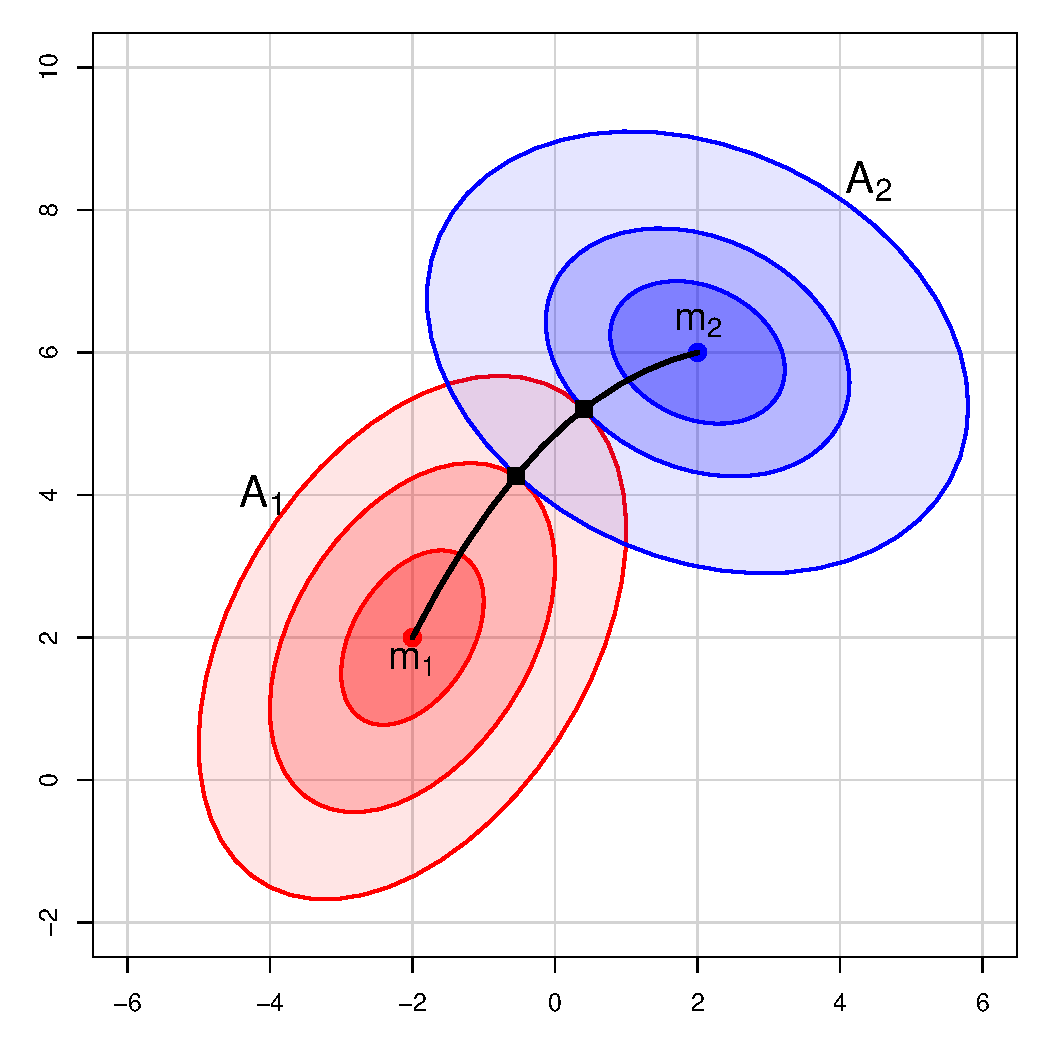
\includegraphics[width=.6\textwidth,clip]{fig/kiss-demo}
  \caption{Locus of osculation for two families of ellipsoidal level curves, with centers at $\vec{m}_1 = (-2, 2)$ and  $\vec{m}_2 = (2, 6)$,
  and shape matrices $\mat{A}_1$ and $\mat{A}_2$ given in \eqref{eq:kiss-demoA}.
  The left ellipsoids (red) have radii=1, 2, 3. The right ellipsoids
  have radii=1, 1.74, 3.1, where the last two values were chosen to make them kiss at the points marked with squares. The black curve is an
  approximation to the path of osculation, using a
  spline function connecting $\vec{m}_1$ to $\vec{m}_2$ via the marked points of osculation.}%
  \label{fig:kiss-demo}
\end{figure}

A general solution can be described as follows.  Let the ellipses be given by
\begin{eqnarray*}
f_1(\vec{x}) & = & \vec{m}_1 \oplus \sqrt{\mat{A}_1} = (\vec{x}-\vec{m}_1)\trans \mat{A}_1 (\vec{x}-\vec{m}_1) \\
f_2(\vec{x}) & = & \vec{m}_2 \oplus \sqrt{\mat{A}_2} = (\vec{x}-\vec{m}_2)\trans \mat{A}_2 (\vec{x}-\vec{m}_2) \comma \\
\end{eqnarray*}
and denote their gradient-vector functions as
\begin{equation}
\nabla f(x_1, x_2) = \left(\frac{\partial f}{\partial x_1}, \frac{\partial f}{\partial x_2} \right)
\end{equation}
so that
\begin{eqnarray*}
\nabla f_1(\vec{x}) & = & 2 \mat{A}_1 (\vec{x}-\vec{m}_1) \\
\nabla f_2(\vec{x}) & = & 2 \mat{A}_2 (\vec{x}-\vec{m}_2) \period \\
\end{eqnarray*}

Then, the points where $\nabla f_1$ and $\nabla f_2$ are parallel can be expressed in terms of the
condition that their vector cross product,
$\vec{u} \circledast \vec{v} = u_1 v_2 - u_2 v_1 = \vec{v}\trans \mat{C} \vec{u} = 0$, where \mat{C} is the skew-symmetric matrix
\begin{equation*}
\mat{C} = \left(
\begin{array}{cc}
 0 & 1 \\ -1 & 0
\end{array}
\right)
\end{equation*}
satisfying $\mat{C} = -\mat{C}\trans$.
Thus, the locus of osculation is the set $\mathcal{O}$, given by $\mathcal{O}  = \{\vec{x} \in \Real{2} \given \nabla f_1(\vec{x}) \circledast \nabla f_2(\vec{x}) = 0 \}$,
which implies
\begin{equation}
(\vec{x}-\vec{m}_2)\trans \, \mat{A}_2 \trans \: \mat{C} \: \mat{A}_1 \, (\vec{x}-\vec{m}_1) = 0  \period  \label{eq:locus}
\end{equation}
\eqref{eq:locus} is a biquadratic form in \vec{x}, with central matrix $\mat{A}_2 \trans \: \mat{C} \: \mat{A}_1$,
implying that $\mathcal{O}$ is a conic section in the general case. Note that when $\vec{x}=\vec{m}_1$ or $\vec{x}=\vec{m}_2$,
\eqref{eq:locus} is necessarily zero, so the locus of osculation always passes through  $\vec{m}_1$ and $\vec{m}_2$.

A visual demonstration of the theory above is
shown in \figref{fig:kiss-demo2} (left), which overlays the ellipses in \figref{fig:kiss-demo} with contour lines
(hyperbolae, here)
of
the vector cross-product function contained in \eqref{eq:locus}.
When the contours of $f_1$ and $f_2$ have the same shape ($\mat{A}_1 = c \mat{A}_2 $), as in the right panel of \figref{fig:kiss-demo2},
\eqref{eq:locus}
reduces to a line, in accord with the stones-in-pond interpretation.
The above can be readily extended to ellipsoids in higher dimension, where the development is more easily understood
in terms of normals to the surfaces.

\begin{comment}
\begin{figure}[htb!]
  \centering
  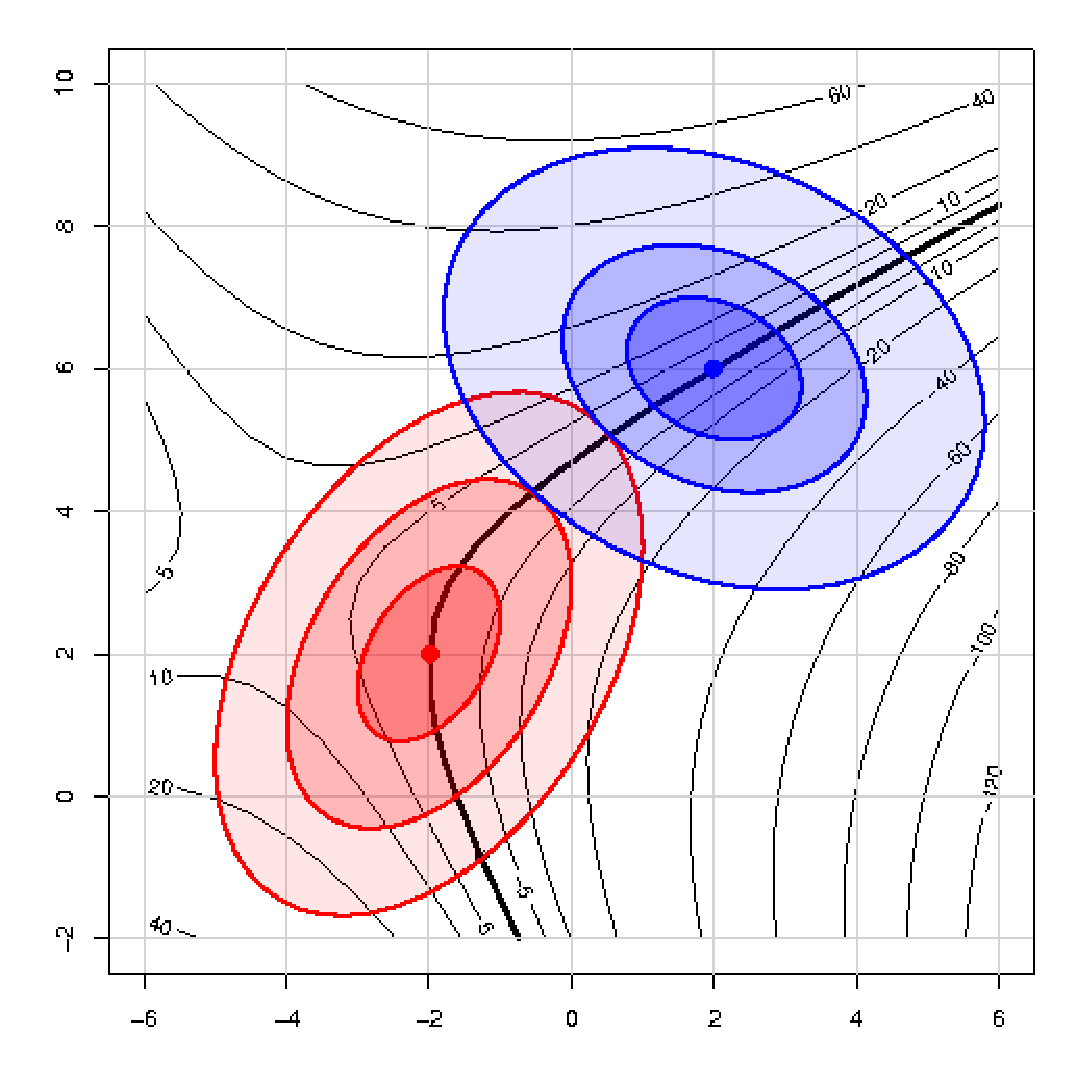
\includegraphics[width=.6\textwidth,clip]{fig/kiss-demo2}
  \caption{Locus of osculation for two families of ellipsoidal level curves, with parameters as in \figref{fig:kiss-demo} and \eqref{eq:kiss-demoA},
  showing contour lines of the vector cross-product function \eqref{eq:locus}.
  The thick black curve shows the complete locus of osculation for these two families of ellipses.}%
  \label{fig:kiss-demo2}
\end{figure}
\end{comment}

\begin{figure}[htb]
 \begin{minipage}[b]{.49\linewidth}
  \centering
  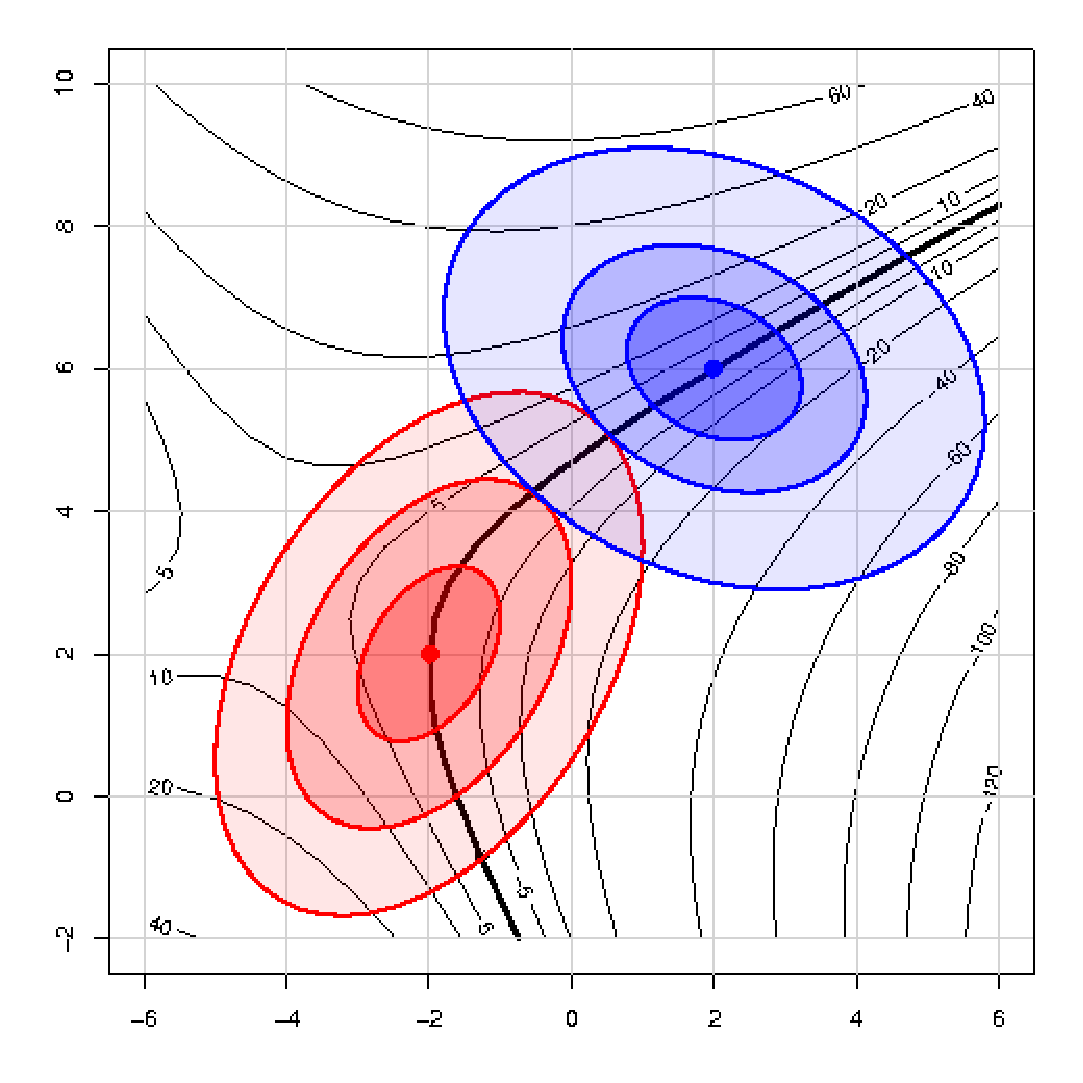
\includegraphics[width=1\linewidth]{fig/kiss-demo2a}
%  \caption{}%
%  \label{fig:}
 \end{minipage}%
 \hfill
 \begin{minipage}[b]{.49\linewidth}
  \centering
  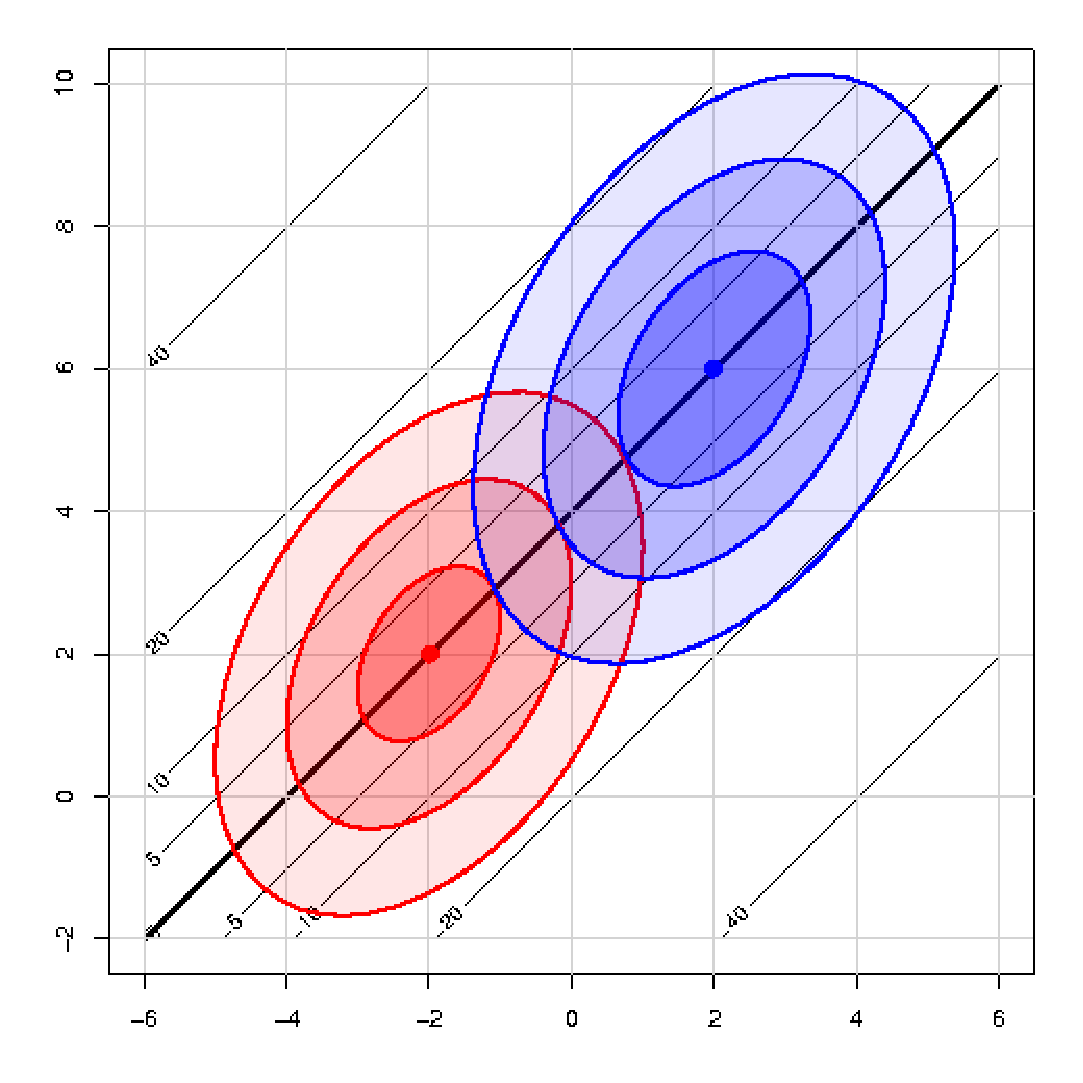
\includegraphics[width=1\linewidth]{fig/kiss-demo2b}
 \end{minipage}
  \caption{Locus of osculation for two families of ellipsoidal level curves, showing contour lines of the vector cross-product function \eqref{eq:locus}.
  The thick black curve shows the complete locus of osculation for these two families of ellipses, where the cross-product function equals 0.
Left:~with parameters as in \figref{fig:kiss-demo} and \eqref{eq:kiss-demoA}. Right:~with the same shape matrix $\mat{A}_1$ for both
ellipsoids.}
  \label{fig:kiss-demo2}
\end{figure}
%\end{document}

\subsection{Discriminant analysis}

The right panel of \figref{fig:kiss-demo2}, considered in data space, provides a
visual interpretation of the classical, normal theory two-group discriminant analysis problem.
Here, we imagine that the plot shows the contours of data ellipsoids for two groups,
with mean vectors $\vec{m}_1$ and $\vec{m}_2$, and common covariance matrix
$\mat{A} = \mat{S}_{\textrm{pooled}} = [ (n_1 -1)\mat{S}_1 + (n_2 -1)\mat{S}_2 ] / (n_1 +n_2 -2) $.

The discriminant axis is the locus of osculation between the two families of ellipsoids.
The goal in discriminant analysis, however, is to determine a classification rule based on
a linear function, $\mathcal{D}(\vec{x}) = \vec{b}\trans \vec{x}$, such that
an observation $\vec{x}$ will be classified as belonging to Group 1 if
$\mathcal{D}(\vec{x}) \le d$, and to Group 2 otherwise.  In linear discriminant
analysis, the discriminant function coefficients are
given by
\begin{equation*}
\vec{b} = \mat{S}_{\textrm{pooled}}^{-1} ( \vec{m}_1 - \vec{m}_2 ) \period
\end{equation*}

All boundaries
of the classification regions determined by $d$
will then be the tangent lines (planes) to the ellipsoids at points of osculation.
The location of the classification region along the line from $\vec{m}_1$ to $\vec{m}_2$
typically takes into account both the
prior probabilities of membership in Groups 1 and 2, and the costs of misclassification.





\subsection{Ridge regression}\label{sec:ridge}

In the univariate linear model, $\vec{y} = \mat{X} \vec{\beta} + \vec{\epsilon}$,
high multiple correlations among the predictors in \mat{X} lead to problems
of \emph{collinearity}---unstable OLS
estimates of the parameters in \vec{\beta} with inflated standard errors
and coefficients that tend to be too large in absolute value.
Although collinearity is essentially a data problem
\citep{Fox:2008},
one popular (if questionable) approach is ridge regression, which shrinks the estimates toward
\vec{0} (introducing bias) in an effort to reduce sampling variance.


Suppose the predictors and response have been centered at their means and the unit vector is
omitted from \mat{X}. Further, rescale the columns of \mat{X} to unit length, so that $\mat{X}\trans \mat{X}$ is a correlation matrix.
% and scaled by their standard deviations and that the response has been centered.
Then, the OLS estimates are given by
\begin{equation}
\widehat{\vec{\beta}}^{\mathrm{OLS}} = (\mat{X}\trans \mat{X})^{-1} \mat{X}\trans \vec{y} \period
\end{equation}
Ridge regression replaces the standard residual sum of squares criterion with a penalized
form,
\begin{equation}
\mathrm{RSS}(k) = (\vec{y}-\mat{X} \vec{\beta}) \trans  (\vec{y}-\mat{X} \vec{\beta}) + k \vec{\beta}\trans\vec{\beta} \quad\quad (k \ge 0)
 \comma \label{eq:ridgeRSS}
\end{equation}
whose solution is easily seen to be
%\begin{equation}
%\widehat{\vec{\beta}}_{\mathrm{RR}} = (\mat{X}\trans \mat{X} + k \mat{I})^{-1} \mat{X}\trans \vec{y} \period
%\end{equation}

\begin{eqnarray}
\widehat{\vec{\beta}}^{\mathrm{RR}}_k  & = &(\mat{X}\trans \mat{X} + k \mat{I})^{-1} \mat{X}\trans \vec{y}  \label{eq:ridge-beta} \\
                                    & = & \mat{G} \, \widehat{\vec{\beta}}^{\mathrm{OLS}}  \nonumber \comma
\end{eqnarray}
where $\mat{G} = \left[\mat{I} + k (\mat{X}\trans \mat{X})^{-1} \right] ^{-1}$.
Thus, as the ``ridge constant'' $k$ increases, \mat{G} decreases, driving $\widehat{\vec{\beta}}^{\mathrm{RR}}_k$ toward \vec{0}
\citep{HoerlKennard:1970a,HoerlKennard:1970b}.  The addition of a positive constant $k$ to the diagonal of $\mat{X}\trans\mat{X}$
drives $\det{\mat{X}\trans\mat{X}+ k \mat{I}}$ away from zero even if $\det{\mat{X}\trans\mat{X}}\approx 0$.

\begin{figure}[htb!]
  \centering
  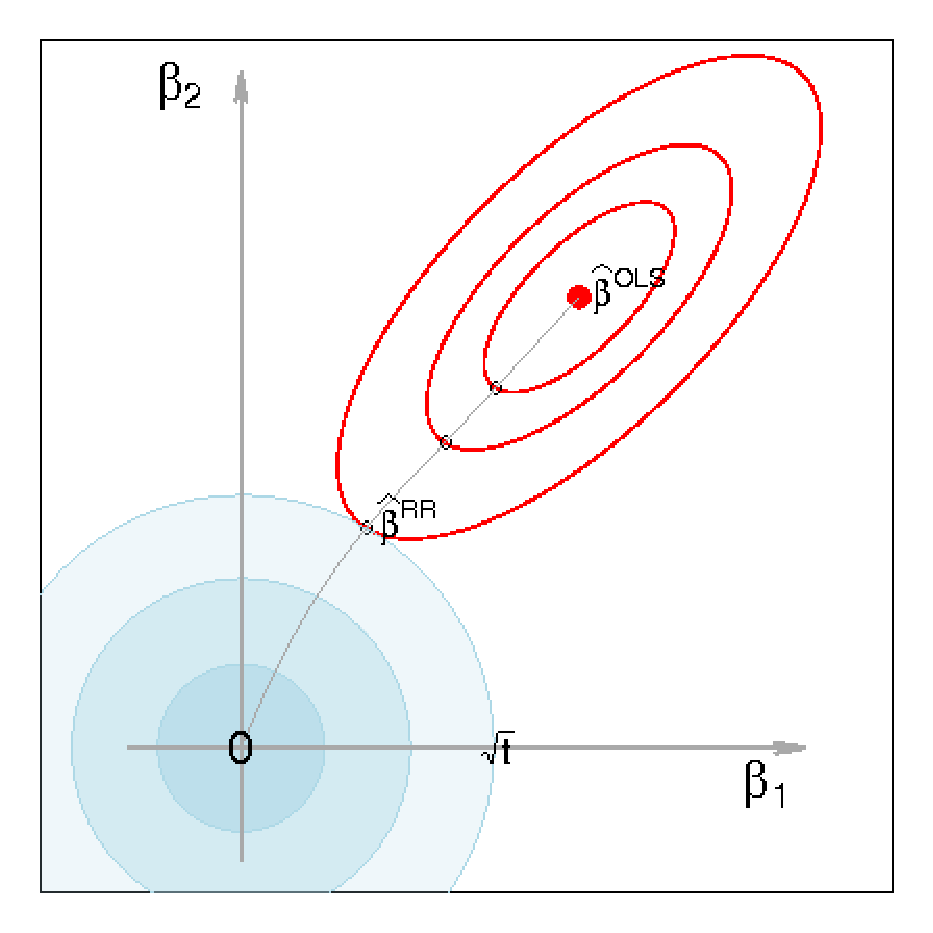
\includegraphics[width=.6\textwidth,clip]{fig/ridge-demo}
  \caption{Elliptical contours of the OLS residual sum of squares for two parameters in a regression, together with
  circular contours for the constraint function, $\beta_1^2 + \beta_2^2 \le t$. Ridge regression finds the point $\vec{\beta}^{RR}$ where
  the OLS contours just kiss the contstraint region.}%
  \label{fig:ridge-demo}
\end{figure}
The penalized Lagrangian formulation in \eqref{eq:ridgeRSS} has an equivalent form as a constrained
minimization problem,
\begin{equation}
\widehat{\vec{\beta}}^{\mathrm{RR}} = \argmin_{\vec{\beta}} (\vec{y}-\mat{X} \vec{\beta}) \trans  (\vec{y}-\mat{X} \vec{\beta})
  \quad\quad\mbox{subject to}\quad\quad
   \vec{\beta}\trans \vec{\beta} \le t(k)  \comma \label{eq:ridge}
\end{equation}
which makes the size constraint on the parameters explicit, with $t(k)$ an inverse function of $k$. This form provides
a visual interpretation of ridge regression, as shown in \figref{fig:ridge-demo}. Depicted in the figure are the
elliptical contours of the OLS regression sum of squares, $\mathrm{RSS}(0)$ around $\widehat{\vec{\beta}}^{\mathrm{OLS}}$.  Each
ellipsoid marks the point closest to the origin, i.e., with $\min \vec{\beta}\trans \vec{\beta}$.
It is easily seen that the ridge regression solution is the point where the elliptical contours just kiss the
constraint contour.

Another insightful interpretation of ridge regression \citep{Marquardt:1970} sees the ridge estimator as equivalent to
an OLS estimator, when the actual data in \mat{X} are supplemented by some number of fictitious observations, $n(k)$,
with uncorrelated predictors,
giving rise to
an orthogonal $\mat{X}_k^0$ matrix, and where $y=0$ for all supplementary observations. The linear model then becomes,

\begin{equation} \label{eq:ridge-sup1}
\left(
\begin{array}{c} \vec{y} \\ \vec{0} \end{array}
\right)
=
\left(
\begin{array}{c} \mat{X} \\ \mat{X}_k^0 \end{array}
\right)
\vec{\beta}^{\mathrm{RR}} + 
\left(
\begin{array}{c} \vec{e} \\ \vec{e}_k^0 \end{array}
\right)
\comma
\end{equation}
which gives rise to the solution,
\begin{equation} \label{eq:ridge-sup2}
\widehat{\vec{\beta}}^{\mathrm{RR}} = [\mat{X}\trans \mat{X} + (\mat{X}_k^0)\trans \mat{X}_k^0]^{-1} \mat{X}\trans \vec{y} \period
\end{equation}
But because $\mat{X}_k^0$ is orthogonal, $(\mat{X}_k^0)\trans \mat{X}_k^0$ is a scalar multiple of \mat{I}, so there
exists some value of $k$ making \eqref{eq:ridge-sup2} equivalent to \eqref{eq:ridge-beta}.  As promised, the
ridge regression estimator then reflects a weighted average of the data $[\mat{X}, \vec{y}]$ with $n(k)$ observations
$[\mat{X}_k^0, \vec{0}]$
biased toward $\vec{\beta}=\vec{0}$. In \figref{fig:ridge-demo}, it is easy to imagine that there is a direct translation between
the size of the constraint region, $t(k)$, and an equivalent supplementary sample size, $n(k)$, in this interpretation.

This classic version of the ridge regression problem can be generalized in a variety of ways, giving other geometric
insights.  Rather than a constant multiplier $k$ of \vec{\beta}\trans \vec{\beta} as the penalty term in \eqref{eq:ridgeRSS},
consider a penalty of the form $\vec{\beta}\trans \mat{K} \vec{\beta}$ with
a positive definite matrix \mat{K}.
The choice $\mat{K} = \diag (k_1, k_2, \dots)$ gives rise to a version of
\figref{fig:ridge-demo} in which the constraint contours are ellipses aligned with the coordinate axes, with
axis lengths inversely proportional to $k_i$.  These constants allow for differential shrinkage of the OLS coefficients.
The visual solution to the obvious modification of \eqref{eq:ridge} is again the point where the elliptical
contours of $\mathrm{RSS}(0)$ kiss the contours of the (now elliptical) constraint region.




\subsubsection{Bivariate ridge trace plots}

Ridge regression is touted as a method to counter the effects
of collinearity by trading off a small amount of bias for an
advantageous decrease in variance.  The results are often 
visualized in a a \emph{ridge trace plot}
\citep{HoerlKennard:1970b},
showing the changes
in individual coefficient estimates as a function of $k$.
A bivariate version of this plot, with confidence ellipses for
the parameters is introduced here.  This plot provides greater
insight on the effects on \emph{both} bias and variance.

In the standard linear model, confidence ellipsoids are generated
from the estimated covariance matrix of the of the parameters,
\begin{equation*}
\widehat{\Var} (\vec{\beta}^{OLS}) = \hat{\sigma}^2_e (\mat{X}\trans \mat{X})^{-1} \period
\end{equation*}
In the ridge regression model, this becomes 
%(Marquandt, 1970)
\citep{Marquardt:1970}
\begin{equation}
\widehat{\Var} (\vec{\beta}^{RR}) = \hat{\sigma}^2_e 
    [\mat{X}\trans \mat{X} + k \mat{I}]^{-1}
    (\mat{X}\trans \mat{X})
    [\mat{X}\trans \mat{X} + k \mat{I}]^{-1} \comma
%    = \mat{G}  (\mat{X}\trans \mat{X}) \mat{G} \comma
\end{equation}
which coincides with the OLS result when $k=0$.
	
\begin{figure}[htb!]
  \centering
  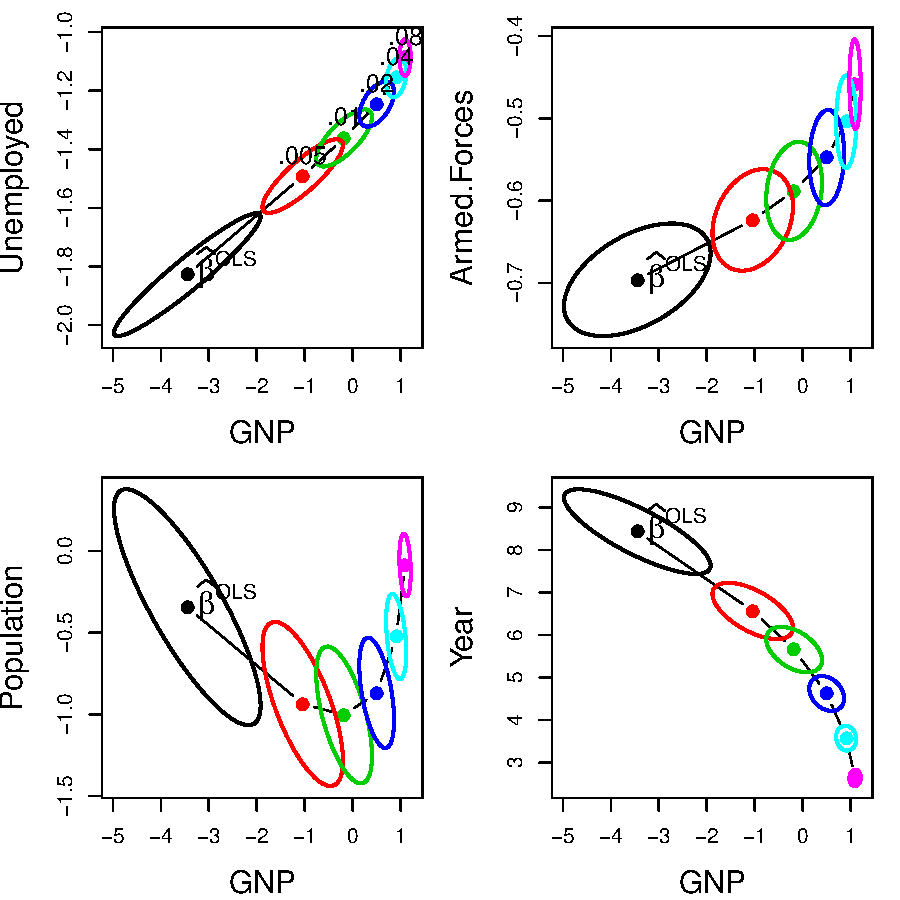
\includegraphics[width=\textwidth,clip]{fig/ridge2}
  \caption{Bivariate ridge trace plots for the coefficients of four predictors
  	against the coefficient for GNP in Longley's data, with
  	$k = 0, 0.005, 0.01, 0.02, 0.04, 0.08$.
  	In most cases the coefficients are driven toward zero, but the bivariate
  	plot also makes clear the reduction in variance.
  	To reduce overlap, all confidence ellipses are shown with 1/2 the standard radius.}%
  \label{fig:ridge2}
\end{figure}

\figref{fig:ridge2} uses the classic \citet{Longley:1967}
data to illustrate
bivariate ridge trace plots.  The data consist of an economic time series ($n=16$)
observed yearly from 1947 to 1962, with the number of people Employed as the
response and the following predictors:
GNP, Unemployed,  Armed.Forces,  Population,  Year,  GNP.deflator (using
1954 as 100).% 
\footnote{
\citet{Longley:1967} used these data to demonstrate the effects of 
numerical instability and round-off error in least squares computations
based on direct computation of the crossproducts matrix, $\mat{X}\trans\mat{X}$.
This sparked the development of a wide variety of
numerically stable least squares algorithms (QR, modified Gram-Schmidt, etc.)
now used is almost all statistical software.
Even ignoring numerical problems 
(not to mention problems due to lack of independence), these
data would be expected to exhibit high collinearity because  
a number of the predictors would be expected to have strong associations
with year and/or population, yet both of these are also included among the
predictors.
}
The standard linear model for these data, in R notation
is \verb|lm(Employed ~ ., data=longley)|.  For each value of $k$, the plot 
shows the estimate $\widehat{\vec{\beta}}$, together with the confidence
ellipse.  For the sake of this example, we assume that GNP is a primary
predictor of Employment, and we wish to know how other predictors modify the
regression estimates and their variance when ridge regression is used.

For this data, it can be seen that even small values of $k$ have substantial
impact on the estimates $\widehat{\vec{\beta}}$. What is perhaps more dramatic
(and unseen in univariate trace plots) is the impact on the size of the confidence
ellipse.  Moreover, shrinkage in variance is generally in a similar direction to the
shrinkage in the coefficients.


%\subsection{Bayesian models}
\subsection{Bayesian linear models}\label{sec:bayesian}

In a Bayesian alternative to standard least squares estimation, consider the case where our prior
information about \vec{\beta} can be encapsulated in a distribution with a prior mean
$\vec{\beta}^{\mathrm{prior}}$ and covariance matrix \mat{A}.  We show that under reasonable conditions
the Bayesian posterior
estimate, $\widehat{\vec{\beta}}^{\mathrm{posterior}}$, turns out
to be a weighted average of the prior coefficients $\vec{\beta}^{\mathrm{prior}}$ and the OLS solution $\widehat{\vec{\beta}}^{\mathrm{OLS}}$,
with weights proportional to the conditional prior precision, $\mat{A}^{-1}$, and the data precision given by
$\mat{X}\trans\mat{X}$.   Once again, this can be understood geometrically as the locus of osculation of
ellipsoids that characterize the prior and the data.

Under Gaussian assumptions,
the conditional likelihood can be written as
\begin{equation*}
\mathcal{L} (\vec{y} \given \mat{X}, \vec{\beta}, \sigma^2) \propto
   (\sigma^2)^{-n/2} \; \exp \left[ -\frac{1}{2 \sigma^2} (\vec{y}-\mat{X} \vec{\beta}) \trans  (\vec{y}-\mat{X} \vec{\beta})   \right] \period
\end{equation*}
To focus on alternative estimators, we can complete the square around $\widehat{\vec{\beta}} = \widehat{\vec{\beta}}^{\mathrm{OLS}}$ to give

\begin{equation} \label{eq:bayes-qform}
(\vec{y}- \mat{X} \vec{\beta})\trans(\vec{y}- \mat{X} \vec{\beta}) =
(\vec{y}- \mat{X} \widehat{\vec{\beta}})\trans(\vec{y}- \mat{X} \widehat{\vec{\beta}}) +
(\vec{\beta} - \widehat{\vec{\beta}})\trans(\mat{X}\trans\mat{X})(\vec{\beta} - \widehat{\vec{\beta}}) \period
\end{equation}
With a little manipulation, a conjugate prior, of the form $\Pr (\vec{\beta}, \sigma^2) = \Pr (\vec{\beta} \given \sigma^2) \times \Pr (\sigma^2)$
can be expressed with $\Pr (\sigma^2)$ an inverse gamma distribution depending on the first term on the right hand side of \eqref{eq:bayes-qform}
and $\Pr (\vec{\beta} \given \sigma^2)$ a normal distribution,
\begin{equation}
\Pr (\vec{\beta} \given \sigma^2) \propto (\sigma^2)^{-p}  \times \exp \left[ -\frac{1}{2 \sigma^2}  (\vec{\beta} - \vec{\beta}^{\mathrm{prior}}) \trans  \: \mat{A} (\vec{\beta} - \vec{\beta}^{\mathrm{prior}})  \right] \period
\end{equation}

The posterior distribution is then
$\Pr (\vec{\beta}, \sigma^2 \given \vec{y}, \mat{X}) \propto \Pr (\vec{y} \given \mat{X}, \vec{\beta}, \sigma^2) \times
\Pr (\vec{\beta} \given \sigma^2) \times \Pr (\sigma^2)$,
whence, after some simplification,
the posterior mean can be expressed as

\begin{equation}\label{eq:bayes-posterior}
\widehat{\vec{\beta}}^{\mathrm{posterior}} =
(\mat{X}\trans \mat{X}\widehat{\vec{\beta}}^{\mathrm{OLS}} + \mat{A} \vec{\beta}^{\mathrm{prior}})
(\mat{X}\trans \mat{X}+\mat{A})^{-1}
\end{equation}
with covariance matrix $(\mat{X}\trans \mat{X}+\mat{A})^{-1}$. The posterior coefficients are thus a weighted average of
the prior coefficients and the OLS estimates, with weights given by the conditional prior precision, $\mat{A}^{-1}$,
and the data precision, $\mat{X}\trans\mat{X}$.  Thus, as we increase the strength of our prior precision (decreasing
prior variance), we place greater weight on our prior beliefs relative to the data.

In this context, ridge regression can be seen as the special case where $\widehat{\vec{\beta}}^{\mathrm{prior}} = \vec{0}$ and $\mat{A} = k \mat{I}$
and where \figref{fig:ridge-demo} provides an elliptical visualization. In \eqref{eq:ridge-sup2}, the number of observations,
$n(k)$ corresponding to $\mat{X}_k^0$ can be seen as another way of expressing the weight of the prior in relation to the data.

% \TODO{Complete this section.  What have I omitted in the development, necessary for this paper?
% Are there other geometric insights?  Does it need another, Bayesian specific graph?
% Is there a simple expression for $\Var({\widehat{\vec{\beta}}^{\mathrm{posterior}}})$
% that could be exploited?
% }




%\subsection{Mixed models: BLUEs and BLUPs}
\subsection{Mixed models: BLUEs and BLUPs}
\TODO{This section, and the incomplete example that follows is just an initial attempt,
awaiting a more insightful description.}

In this section we make use of the duality between data space and $\beta$
space, where lines in one map into points in the other and ellipsoids to
visualize the precision of estimates in the context of the general linear mixed
model for hierarchical data.  We also show visually how the best linear unbiased
predictors (BLUPs) from the mixed model can be seen as a weighted average
of OLS regression, best linear unbiased estimates (BLUEs) \emph{within} strata
and the variation of random effect estimates \emph{between} strata.

The mixed model for hierarchical data provides a general framework for 
dealing with lack of independence among observations in linear models,
such as occurs when students are sampled within schools, schools within
counties and so forth. In these situations, the assumption of OLS that
the residuals are conditionally independent is likely to be violated,
because, for example, students nested within the same school are 
likely to have more similar outcomes than those from separate schools.


\subsubsection{Example: Math achievement and SES}

To illustrate, we use a classic data set from %Bryk \& Raudenbush (2002)
\citet{BrykRaudenbush:1992} and \citet{RaudenbushBryk:2002}
dealing with math achievement scores for a subsample of 7,185 students from 160 schools
in the 1982 High School \& Beyond survey of U.S. public and Catholic high
schools conducted by the National Center for Education Statistics (NCES).
The data set contains 90 public schools and 70 Catholic schools, with
sample sizes ranging from 14 to 67.

The response is a standardized measure of math achievement, while
student-level predictor variables include sex and student socioeconomic status (SES), and
school-level predictors include sector (public or Catholic) and mean SES for the
school (among other variables).
Following \citet{RaudenbushBryk:2002}, student SES is considered the main predictor, and is
typically analyzed centered within schools,
$\mathrm{CSES}_{ij} = \mathrm{SES}_{ij} - \mathrm{(mean SES)}_i$, for ease of interpretation (making the within-school intercept for school $i$
equal to the mean SES in that school).



\begin{figure}[htb]
 \begin{minipage}[b]{.49\linewidth}
  \centering
  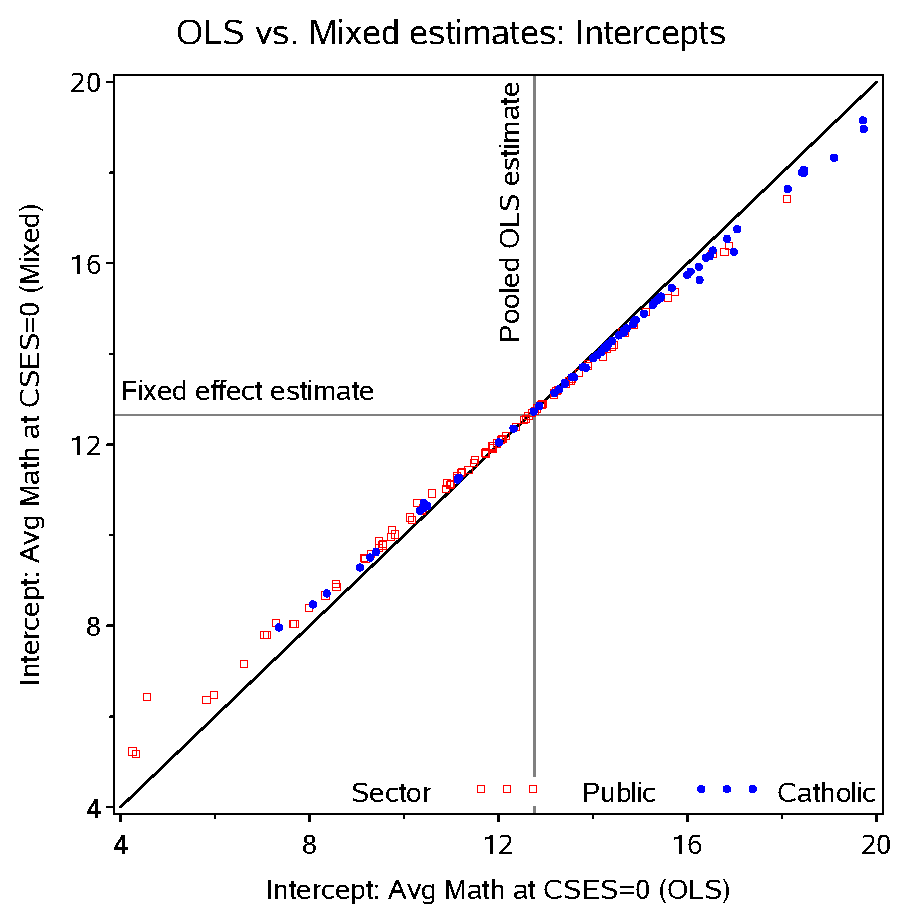
\includegraphics[width=1\linewidth,clip]{fig/hsbmix41}
%  \caption{}%
%  \label{fig:}
 \end{minipage}%
 \hfill
 \begin{minipage}[b]{.49\linewidth}
  \centering
  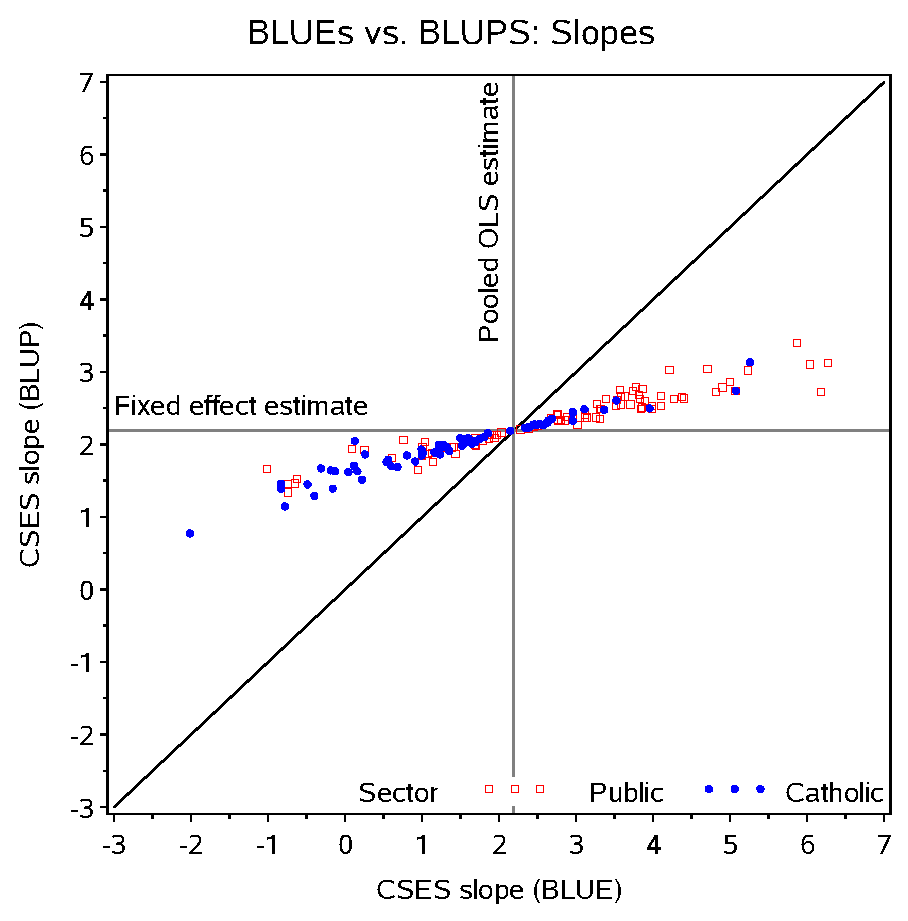
\includegraphics[width=1\linewidth,clip]{fig/hsbmix42}
 \end{minipage}
  \caption{Comparing BLUEs and BLUPs. Each panel plots the OLS estimates from separate regressions for each school (BLUEs)
  versus the mixed model estimates from the random intercepts and slopes model (BLUPs).
  Left: intercepts; Right: slopes for CSES.  The shrinkage of the BLUPs toward the OLS estimate is much greater for slopes than
  intercepts. }
  \label{fig:hsbmix4}
\end{figure}

For simplicity, we consider the case of CSES as
a single quantitative predictor in $\mat{X}$ in the example below.  We fit and compare the following models:
\begin{eqnarray}
 \vec{y}_{i} & \sim & \mathcal{N} ( \beta_0 + x_{i} \beta_1 , \sigma^2 ) \quad\quad \textrm{pooled OLS} \\
 \vec{y}_{i} & \sim & \mathcal{N} ( \beta_{0i} + x_{i} \beta_{1i} , \sigma^2_i ) \quad\quad \textrm{unpooled BLUEs} \\
 \vec{y}_{i} & \sim & \mathcal{N} ( \beta_{0} + x_{i} \beta_{1} + u_{0i} + x_{i} u_{1i} , \sigma^2_i ) \quad\quad \textrm{BLUPs: random intercepts and slopes}
%
\end{eqnarray}
and also include a fixed effect of sector, common to all models; for compactness, the sector effect is elided in the notation above.

In expositions of mixed-effects models, such models are often compared visually by plotting predicted values in data space, where each school appears
as a fitted line under one of the models above (sometimes called ``spaghetti plots'').
Our geometric approach leads us to consider the equivalent but simpler plots in the dual $\beta$ space,
where each school appears as a point.

\figref{fig:hsbmix4} plots the unpooled BLUE estimates against the BLUPs from the random effects model, with separate panels for intercepts
and slopes to illustrate the shrinkage of different parameters.  In these data, the variance in intercepts (average math achievement
for students at $\mathrm{CSES}=0$), $g_{00}$,
among schools in each sector is large, so the mixed effects estimates have small weight and there is little
shrinkage.  On the other hand, the variance component for slopes, $g_{11}$, is relatively small, so there is greater
shrinkage toward the BLUE, fixed effect estimate.

\begin{figure}[htb!]
  \centering
  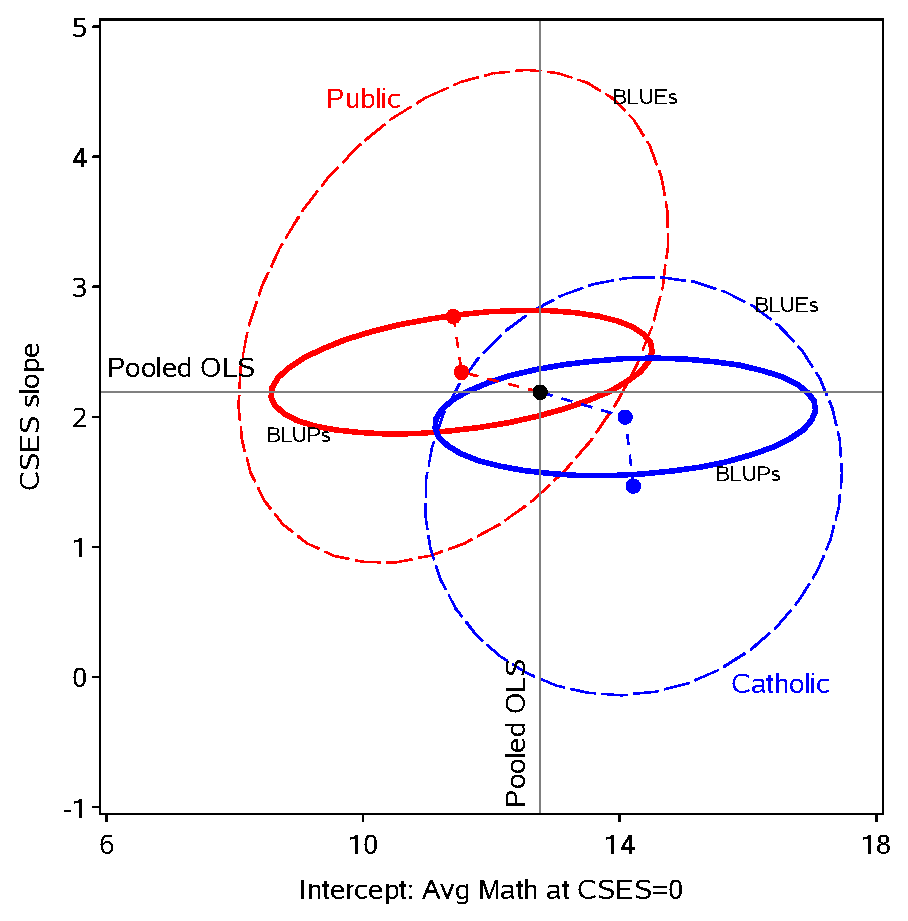
\includegraphics[width=.6\textwidth,clip]{fig/hsbmix43}
  \caption{Comparing BLUEs and BLUPs. The plot shows ellipses of 50\% coverage for the estimates of intercepts and slopes
  from OLS regressions (BLUEs) and the mixed model (BLUPs), separately for each sector.
  The centers of the ellipses illustrate how the BLUPS can be considered a weighted average of the BLUEs and the
  pooled OLS estimate, ignoring sector. The relative sizes of the ellipses reflect the smaller variance for the
  BLUPs compared to the BLUEs, particularly for slope estimates. }%
  \label{fig:hsbmix43}
\end{figure}

For the present purposes, a more useful visual representation of these model comparisons can be shown together in
the space of $(\beta_0, \beta_1)$, as in \figref{fig:hsbmix43}.  Estimates for individual schools are not shown,
but rather these are summarized by the ellipses of 50\% coverage for the BLUEs and BLUPs within each sector.
The centers of the ellipsoids indicate the relatively greater shrinkage of slopes compared to intercepts.
The sizes of ellipsoids show directly the greater precision of the BLUPs, particularly for slopes.


\section{Discussion and Conclusions}

\epigraph{I know of scarcely anything so apt to impress the imagination as the
wonderful form of cosmic order expressed by the ``[Elliptical] Law of Frequency of
Error.''
The law would have been personified by the Greeks and deified, if they had known of it.
... % It reigns with serenity and in complete self-effacement, amidst the wildest confusion.
    % The huger the mob, and the greater the apparent anarchy, the more perfect is its sway.
    It is the supreme law of Unreason.
	Whenever a large sample of chaotic elements are taken in hand
	and marshaled in the order of their magnitude,
	an unsuspected and most beautiful form of regularity proves to have been
	latent all along.
}
{Sir Francis Galton, \emph{Natural Inheritance}, London: Macmillan, 1889
(``[Elliptical]'' added).
%Quoted in J. R. Newman (ed.) The World of Mathematics, New York: Simon and Schuster, 1956. p. 1482.
}

We have taken the liberty to add the word ``Elliptical'' to this famous quotation from Galton (1889).
His ``supreme law of Unreason'' referred to univariate distributions of observations tending to the
Normal distribution in large samples.  We believe he would not take us remiss, and might perhaps
welcome us for extending this view to
two and more dimensions, where ellipsoids often provide
an ``unsuspected and most beautiful form of regularity.''

In statistical data, theory, and graphical methods, one main organizing
distinction can be made depending
on the dimensionality of the problem.  A coarse but useful scale considers the essential defining
distinctions to be among
\begin{itemize*}
 \item ONE (univariate),
 \item TWO (bivariate),
 \item MANY (multivariate).
\end{itemize*}
This scale%
\footnote{
This idea, as a unifying classification principle for data analysis and graphics,
was first suggested to the first author in
seminars by John Hartigan at Princeton, c.~1968.
}
at least implicitly organizes much of current statistical teaching, practice, and software.
But within this classification, the data, theory, and graphical methods are often treated separately (1D, 2D, $n$D),
without regard to geometric ideas and visualizations that help to unify them.

This paper starts from the premise that one geometric form---the ellipsoid---provides a unifying framework for many statistical phenomena, with simple representations in
1D (a line) and 2D (an ellipse) that extend naturally to higher dimensions (an ellipsoid).  The intellectual leap
in statistical thinking from ONE to TWO in \citet{Galton:1886} was enormous.
Galton's visual insights derived from the ellipse quickly led to an understanding of the
ellipse as a contour of a bivariate normal surface.  From here, the step from TWO to MANY
would take another 20--30 years, but it is hard to escape the conclusion that
geometric insight from the ellipse to the general ellipsoid in $n$D
played an important role in the development of multivariate statistical methods.

In this paper, we have tried to show how ellipsoids can be useful tools for
visual statistical thinking, data analysis, and pedagogy in a variety of contexts often
treated separately and from a univariate perspective.  Even in bivariate
and multivariate problems, first-moment summaries (a 1D regression line
or 2+D regression surface) show only part of the story---that of the
expectation of a response $\vec{y}$ given predictors $\mat{X}$.
In many cases, the more interesting part of the story concerns the
\emph{precision} of various methods of estimation, which we've shown
to be easily revealed through data ellipsoids and
elliptical confidence regions for parameters.

The general relationships among statistical methods, matrix algebra, and geometry are
not new here.  To our knowledge, \citet{Dempster:69} was the first to exploit these relationships
in a systematic fashion, establishing the connections among abstract vector spaces,
algebraic coordinate systems, matrix operations and properties, the dualities
between observation space and variable space,
 and the geometry
of ellipses and projections.%
%\footnote{
%The role of statistical computation should not be underestimated
%in appreciation of Dempster's contribution.
%...
%}
The roots of these connections go back much further---to
\citet{Cramer:1946} (the idea of the concentration ellipsoid), to
\citet{Pearson:1901} and \citet{Hotelling:1933} (principal components),
and, we maintain, ultimately to \citet{Galton:1886}.
Throughout this development, elliptical geometry has played
a fundamental role, leading to important visual insights.

The separate and joint roles of statistical computation and computational graphics should not be underestimated
in appreciation of these developments.  Dempster's analysis of the connections among geometry, algebra, and
statistical methods was fueled by the development and software implementation of algorithms
(Gram-Schmidt orthogonalization, Cholesky decomposition, sweep and multistandardize operators from
\citealp{Beaton:64})
that allowed him to show precisely the translation of theoretical relations
from abstract algebra to numbers and thence to graphs and diagrams.

\citet{Monette:90}
took these ideas several steps further, developing interactive 3D graphics focused on linear
models, geometry, and ellipsoids, and demonstrating how many statistical properties
and results could be understood through the geometry of ellipsoids.  Yet, even at this
later date, the graphical facilities of readily available statistical software were still
rather primitive, and 3D graphics was available only on high-end workstations.


Several features of the current discussion may help to present these ideas in a
new light.  First, the examples we have presented rely heavily on software for
statistical graphics developed separately and jointly by all three authors.
These have allowed us to create what we hope are compelling illustrations,
all statistically and geometrically exact, of the principles and ideas that
form the body of the paper.  Moreover, these are now general methods, implemented
in a variety of R packages
\citep{car,heplots1}
and a large collection of SAS macros (\url{http://datavis.ca/sasmac}),
so we hope this paper will contribute to turning the theory we describe
into practice.

Second, we have illustrated, in a wide variety of contexts,
comprising all classical (Gaussian) linear models, multivariate linear models,
and several extensions,
how ellipsoids can contribute substantially to the understanding of statistical
relationships, both in data analysis and in pedagogy.  One graphical theme underlying
a number of our examples is how the simple addition of ellipses to standard 2D graphical
displays provides an efficient \emph{visual} summary of important bivariate
statistical quantities (means, variances, correlation, regression slopes, etc.)
While first-moment visual summaries are now common adjuncts to graphical displays
in standard software, often by default, we believe that the second-moment visual summaries
of ellipses (and ellipsoids in 3D)
now deserve a similar place in statistical practice.

Finally, we have illustrated several recent or entirely new visualizations of
statistical methods and results, all based on elliptical geometry.
HE plots for MANOVA designs \citep{Friendly:07:manova}
and their projections into canonical space (\secref{sec:mlm})
provide one class of examples where ellipsoids provide simple visual summaries of
otherwise complex statistical results.
Our analysis of the geometry of added variable-plots suggested the idea of superposing
marginal and conditional plots, as in \figref{fig:coffee-avplot-B}, leading to
direct visualization of the difference between marginal and conditional relationships
in linear models.
The bivariate ridge trace plots described in \secref{sec:ridge2} are a direct outgrowth
of the geometric approach taken here, emphasizing the duality between views in data
space and in parameter ($\vec{\beta}$) space.
We believe these all embody von Humboldt's (1811) dictum, quoted in the introduction.







\section{Supplementary materials}

All figures in this paper were constructed with either SAS or R software.
The SAS examples use a collection of SAS macros from \url{http://datavis.ca/sasmac}; the
R examples employ a variety of R packages available from the CRAN web site, \url{http://cran.us.r-project.org/}
and the R-Forge development server at \url{https://r-forge.r-project.org/}.
SAS and R scripts to generate many of the figures are included as supplementary materials for this article.


\section{Acknowledgments}

This work was supported by Grant OGP0138748 from the National Sciences and Engineering Research Council of Canada to Michael Friendly, 
and by grants from the Social Sciences and Humanities Research Council of Canada to John Fox.


%\bibliography{timeref,graphics,Rpackages}
\bibliography{references}        % processed by aux2bib
\end{document}
